\documentclass[twoside,single]{lion-msc}

\title{Inverse Optimal Transport in Cosmological Simulations}
\author{B.A. Sturre}

\affiliation{Leiden Observatory, Leiden University \\
Mathematical Institute, Leiden University}

%\address{P.O. Box 9500, 2300 RA Leiden, The Netherlands}

%\newdate{date}{\day}{\month}{\year}  
\newdate{date}{13}{06}{2025}
%\newdate{date}{\today}
\date{\displaydate{date}}
\studentid{3635066} 
\supervisor{Dr. M. Schaller}
\corrector{Dr. E. Sellentin and} 
\secondmath{Dr. D. van der Hoeven}

% \degree{Bachelor of Science} 
\major{Mathematics and Astronomy}

% optional cover picture - should be jpg or pdf
%\coverpicture{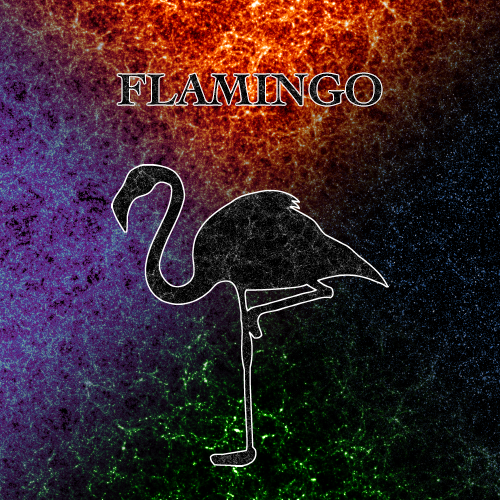
\includegraphics[width=5cm]{FLAMINGO.png}}

\usepackage{tocloft}
\hypersetup{colorlinks=false}
\usepackage{amsmath}
\usepackage{parskip}
\usepackage{enumerate}
\usepackage{url}
\usepackage{float}
\usepackage{amssymb}
\usepackage{graphicx}
\usepackage{amsfonts}
\usepackage{pdfpages}
\usepackage{amstext}
\usepackage{caption}
\usepackage{amsthm}
\usepackage{pdfpages}
\usepackage{color}
\usepackage{listings}
\usepackage{hyperref}
% \usepackage{eufrak}
\usepackage{enumerate}
\usepackage{multicol}
\usepackage{lipsum}
\usepackage{geometry}
\usepackage{comment}
\usepackage{subfig}
\usepackage{subcaption}
\usepackage{bbm}
\usepackage{enumitem}
\usepackage{algorithm2e}
\usepackage{chngcntr}
\usepackage{titlesec}
\usepackage{calc}
\usepackage{sectsty}
\usepackage{natbib}
\usepackage{hyperref}
\geometry{
	a4paper,
	bottom=25mm,
	right=25mm,
	left=25mm,
	top=25mm,
}

\def\N{\mathbb{N}} \def\Z{\mathbb{Z}} \def\Q{\mathbb{Q}} \def\R{\mathbb{R}} \def\C{\mathbb{C}} \def\ra{\rightarrow}
\def\Ra{\Rightarrow} \def\f{\frac} \def\del{\partial} \def\ora{\overrightarrow} \def\si{\;\mathrm} \def\T{\mathcal{T}} \def\P{\mathbb{P}} \def\tab{\;\;\;} \def\E{\mathbb{E}} \def\d{\;\text{d}} \def\L{\mathcal{L}} \def\pihat{\hat{\pi}} \def\C{\mathcal{C}} \def\W{\mathcal{W}} \def\chat{\hat{c}}

\DeclareMathOperator*{\prox}{prox} \DeclareMathOperator*{\argmin}{argmin} \DeclareMathOperator*{\infim}{inf}

\def\tellmewhy{\begin{figure*}[!ht]
		\centering 
		\includegraphics[width=0.15\textwidth]{../../tellmewhy.jpeg}
\end{figure*}}

\definecolor{codegreen}{rgb}{0,0.6,0}
\definecolor{codegray}{rgb}{0.5,0.5,0.5}
\definecolor{codepurple}{rgb}{0.58,0,0.82}
\definecolor{backcolour}{rgb}{0.95,0.95,0.92}


\lstdefinestyle{mystyle}{
	backgroundcolor=\color{backcolour},   
	commentstyle=\color{codegreen},
	keywordstyle=\color{magenta},
	numberstyle=\tiny\color{codegray},
	stringstyle=\color{codepurple},
	basicstyle=\ttfamily\footnotesize,
	breakatwhitespace=false,         
	breaklines=true,                 
	captionpos=b,                    
	keepspaces=true,                 
	numbers=left,                    
	numbersep=5pt,                  
	showspaces=false,                
	showstringspaces=false,
	showtabs=false,                  
	tabsize=2
}

\lstset{style=mystyle}
\RestyleAlgo{ruled}

\titleformat{\chapter}[hang]
{\itshape\huge\bfseries}
{\thechapter.}
{1em}
{}
[\titlerule] 

\sectionfont{\itshape\Large}
\subsectionfont{\itshape\large}
\subsubsectionfont{\itshape\normalsize}
%\paragraphfont{\itshape\small}
%\subparagraphfont{\itshape\small}

\newtheorem{theorem}{Theorem}[chapter]
\newtheorem{definition}[theorem]{Definition}
\newtheorem{lemma}[theorem]{Lemma}
\newtheorem{proposition}[theorem]{Proposition}

\newtheoremstyle{ex}
{\topsep}   
{\topsep}   
{\normalfont}
{0pt}     
{\bfseries}
{.}       
{.5em}     
{}         
\theoremstyle{ex}
\newtheorem{example}[theorem]{Example}
\newtheorem{remark}[theorem]{Remark}

\numberwithin{equation}{chapter}


\hypersetup{
	colorlinks=true,    % False: boxed links; True: colored links
	linkcolor=blue,     % Internal links (sections, etc.)
	citecolor=blue,      % Citations
	urlcolor=magenta    % URLs
}

\abstract{
The theory of Optimal Transport (OT) provides a powerful mathematical framework for understanding dynamics, with applications in various disciplines. In cosmology, OT can offer a unique view through which to analyze structure formation and evolution, by connecting initial and final density configurations.  
In this thesis, we investigate the structure formation in cosmology using an inverse OT approach, focusing on the movement of particles. We utilize data from the FLAMINGO simulations, segmented into smaller boxes for computational efficiency. Our primary objective was to infer the cost matrix that is responsible for the particle motion within these simulations. We developed the theory of inverse OT and developed an algorithm to solve for the cost matrix, while addressing the ill-posed nature of inverse OT. This algorithm is applied to both reference cases and the FLAMINGO simulation data. The derived cost matrix shows a high degree of symmetry, consistent with an isotropic universe. As a proof of concept, a Markov Chain Monte Carlo simulation was done to test if the FLAMINGO cost matrix is a linear combination of reference cases. These Markov chains did not converge. However, this is thought to be because of the limited number of reference cases. 
}  
% limit your self to 1/2 page or 500 words

% texcount final_submission.tex -inc -incbib -sum

\begin{document}
	
\pagenumbering{roman}
\maketitle
\tableofcontents
\cleardoublepage

%\listoffigures
%\newpage
%\listoftables
%\newpage

\pagenumbering{arabic}

\chapter{Introduction}
In the early universe, there were small irregularities in the density of matter. Today, these irregularities can be seen in the Cosmic Microwave Background Radiation \citep{durrer2015}. When gravity starts to act on these small fluctuations, regions that have a slightly higher density will exert a stronger gravitational pull, attracting more matter. This gravitational pull starts off a process where the dense regions will grow denser and the less dense regions will get emptier. Over time, this process leads to the formation of over-dense regions, clusters, and under-dense regions, voids \citep{zeldovich1970}. The formation of these structures have been studied extensively with the use of hydrodynamical simulations \citep{schaye2014, crain2015, schaye2023, kugel2023}, as it is difficult to observe this structure formation directly \citep{bos2016}. \par 
These hydrodynamical simulations have an initial and final particle distribution, often with in-between time-steps. This provides a natural framework for Optimal Transport theory (OT), a rapidly developing area of mathematics. OT allows us to compute distances and relationships between probability distributions \citep{villani2003}. In OT, one looks for the transport of some type of particles (from the initial to the final positions), and tries to minimize the cost this transport takes, making use of some cost function. This cost function is often taken as the work it takes to move particles, possibly with other transport costs, such as fuel costs \citep{villani2008}. \par 
In simulations governed by physical laws, the exact form of cost function is typically unknown, due to the complex gravitational dynamics and non-linear evolution of structures. The reconstruction of initial conditions has been studied within the field of cosmology \citep{nikakhtar2024}, but the inverse OT problem has to our knowledge not been applied in the setting of structure formation in cosmology. Therefore, the goal of this thesis is to reverse the optimal transport process; can we infer the cost function from the observed particle movements?  \par 
To reverse the OT process, data of the FLAMINGO (Full-hydro Large-scale structure simulations with All-sky Mapping for the Interpretation of Next Generation Observations) simulations will be used, see also \citet{schaye2023, kugel2023}. There are different algorithms and methods to recover the cost matrix, each designed for different constraints \citep{stuart2020, ma2021, li2019, chiu2022}. In this thesis, a modified algorithm for unconstrained convex optimization of inverse OT by \citet{ma2021} will be used. \par 
Once we have obtained a cost matrix, we can analyze the shape of the cost matrix to understand the dynamics in the simulations. Furthermore, different cost matrices for different simulations can quantify how the variations of parameters in the simulations affect the dynamics. Lastly, the cost matrix could highlight which physical processes or initial conditions contribute most significantly to the formation of particular structures, such as clusters, filaments or voids. \par 
In this thesis, we will first cover some theoretical foundations of OT and inverse OT in Chapter~\ref{ch:2}, whereafter we will describe the data we will use in more detail in Chapter~\ref{ch:data}. In Chapter~\ref{ch:entropyregiOT}, an algorithm is developed for inverse OT, with comments on the implementation and stability. In Chapter~\ref{ch:results}, the results of the algorithm are discussed for some reference cases, as well as for the FLAMINGO data. 


\chapter[Theoretical Foundations of Optimal Transport]{Theoretical Foundations of \\Optimal Transport}
\label{ch:2}
Before we can work on the problem at hand, we need to properly define what (inverse) Optimal Transport (OT) is. For this, we will first recap a bit of measure theory. \par 
The theory in this chapter is mainly based on \citet{villani2008}, \citet{benamou1998}, \citet{peyre2020} and \citet{chiu2022}. To shorten this chapter, proofs of some statements are left out, they can be found in the mentioned papers.\par

\section{Measure Theory}
The reader is assumed to be familiar with the basic concepts of measure theory. Here, we will introduce a concept that is helpful to understand the language optimal transport theory is formulated in. We will look at the \textit{coupling} of two measures: 
\vspace{0.3cm}
\begin{definition}[Coupling]
	Let $(X, \mu)$ and $(Y, \nu)$ be two probability spaces. By constructing two random variables $X, Y$ on some probability space $(\Omega, \P)$, $\mu$ and $\nu$ are coupled if $\text{law } (X) = \mu$ and $\text{law }(Y) = \nu$, with the couple $(X,Y)$ being called a \textbf{coupling} of $(\mu, \nu)$. 
	\label{def:coupling}
\end{definition}
Here, law$(X)$ is the probability distribution of $X$. By abuse of terminology, the law of $(X,Y)$ is also called a coupling of $(\mu, \nu)$. \par 
If $\mu$ and $\nu$ are the only laws relevant in the problem, we can assume, without loss of generality, $\Omega = X \times Y$. Hence, coupling $\mu$ and $\nu$ means constructing a measure $\pi$ on $X \times Y$ such that $\pi$ admits $\mu$ and $\nu$ as marginals on $X$ and $Y$ respectively. This measure $\pi$ is what we later define as the transportation matrix. 
\vspace{0.3cm}
\begin{definition}[Deterministic coupling]
	Using the same notation as in Definition~\ref{def:coupling}, a coupling $(X, Y)$ is called \textbf{deterministic} if there exists a measurable function $T: X \ra Y$ such that $Y = T(X)$. 
	\label{def:detcoup}
\end{definition}
This is equivalent to saying one of the following statements: 
\begin{itemize}
	\item $(X,Y)$ is a coupling of $\mu$ and $\nu$ whose law $\pi$ is such that $Y$ can be expressed as a measurable function $T$ on $X$ almost everywhere. 
	\item $X$ has law $\mu$ and $Y = T(X)$ where $T_\#\mu = \nu$, with $\#$ the push forward.
\end{itemize}
In Definition~\ref{def:detcoup}, $T$ is uniquely defined $\mu$-almost surely, and is called the \textbf{transport map}.


\section{Monge-Kantorovich Minimization Problem}
Assume we have a pile of sand and a hole we have to fill with the sand. We can model the sand in both the pile and the hole by probability measures $\mu$ and $\nu$, defined om some measure spaces $X$ and $Y$. Let $A\subseteq X$ and $B\subseteq Y$ be measurable subsets of $X$, respectively $Y$. Then, $\mu(A)$ gives a measure of how much sand is located in $A$ and $\nu(B)$ of how much sand is already in $B$. Moving the sand needs some effort, which can be modeled by a measurable \textit{cost function} $c: X \times Y \ra \R \cup \{+ \infty\}$, where we assume the cost to move sand from $A$ to $B$ can be real-valued or infinite. One can then ask the following question, also known as the mass transport problem: how do we realize the transportation of the sand from $A$ to $B$ at minimal cost? This is the question \citet{monge1781} came up with in his \textit{M\'emoire sur la th\'eorie des d\'eblais et des remblais}, which led to the rise of the theory of optimal transport. \par
\vspace{0.3cm}
\begin{example}[Monge-Kantorovich minimization problem]
	The \textbf{optimal coupling} or \textbf{optimal transport} is a coupling where one introduces a \textbf{cost function} $c(x,y)$ on $X \times Y$, that can be interpreted as the work needed to move one unit of mass from location $x$ to location $y$. Then one considers the \textit{Monge-Kantorovich minimization problem}
	\[\infim_{(\mu, \nu) \sim (X,Y)}\; \E \; c(X,Y), \]
	where the pair $(X,Y)$ runs over all possible couplings of $(\mu, \nu)$, or equivalently
	\begin{equation}
		\infim_{\pi \in \Pi(\mu, \nu)} \int_{X \times Y} c(x,y) d\pi(x,y),
		\label{eq:otdef}
	\end{equation}
	where the infimum runs over all joint probability measures $\pi$ on $X \times Y$ with marginals $\mu$ and $\nu$. Such joint measures are called \textit{transference plans} (or transport plans, or transportation plans), and those achieving the infimum are called \textit{optimal transference plans}. 
	\label{ex:ot}
\end{example}
\vspace{0.3cm}
\begin{remark}
	The transference plans in Example~\ref{ex:ot} are couplings as in Definition~\ref{def:coupling}, and they may be deterministic as in Definition~\ref{def:detcoup}. Hence, the problem of Optimal Transport can be rewritten into the question of looking for a (deterministic) optimal coupling.  
\end{remark}
Now, the problem of finding the optimal transport can be reformulated as follows: let $\rho_0$ and $\rho_T$ be bounded, positive and measurable functions with compact support in $\R^d$. We require they integrate to the same number, which can be normalized to $1$: 
\begin{equation}
	\int_{\R^d} \rho_0(x)\; dx = \int_{\R^d} \rho_T(x) \;  dx = 1. 
	\label{eq:normal}
\end{equation}
We then need to find a mapping, or \textit{application}, $M: \R^d \ra \R^d$ which realizes the transport from $\rho_0$ to $\rho_T$. In other words, we need to find an $M$ for which for all $A \in \mathcal{B}(\R^d)$, there holds 
\begin{equation}
	\int_{M^{-1}(A)} \rho_0(x) \; dx = \int_A \rho_T(x)\; dx.
	\label{eq:benamou2}
\end{equation}
Here, $M$ should be achieving the minimal cost of 
\begin{equation}
	\int_{\R^d} c(x, M(x)) \rho_0(x) \; dx. 
	\label{eq:benamou3}
\end{equation}
Note that the condition in equation~\eqref{eq:benamou2} is equivalent to 
\begin{equation}
	\int_{\R^d} f(M(x)) \rho_0(x) \; dx = \int_{\R^d} f(x)\rho_T(x) \; dx
	\label{eq:equivalence}
\end{equation}
for all continuous functions $f$. 
\vspace{0.3cm}
\begin{example}[Cost function]
	Oftentimes, $\rho_0$ and $\rho_T$ are the initial and final density distributions. Then, equation~\eqref{eq:normal} is the requirement of conservation of mass, and the integrals are all in $\R^3$. \par 
	When $\rho_0$ and $\rho_T$ describe density, the cost function $c$ in equation~\eqref{eq:benamou3} is a function that oftentimes is taken as 
	\begin{equation*}
		c: \R^3 \times \R^3 \ra \R, \;\;\; c(x,y) = ||x - y||^r, \label{eq:benamou4}
	\end{equation*}
	for a certain $r > 0$ (as "cost" should increase by distance), with $||\cdot||$ the Euclidean distance in $\R^3$. \par
	A very common value of $r$ for the cost function is $r=2$ \citep{benamou1998}. This choice is often made because the squared Euclidean distance has applications in fluid dynamics and classical mechanics from the kinetic energy term \citep{benamou2000}. \par 
	Our problem then rewrites to finding the cost function $c: \R^3 \times \R^3 \ra \R$ for which equation~\eqref{eq:benamou3} is being minimized under our observed transport. 
\end{example}

\section{Discrete Optimal Transport}
Now, let us look at discrete OT. For now, let us assume our problem has the same initial and final space, $X = Y = \R^n$. Given a cost matrix $c \in \R^{n\times n}$ with elements $c_{i,j}$, OT as in \eqref{eq:benamou2} can be rewritten as the search for a mapping $M$ in the set $\text{Perm}(n)$ of permutations of $n$ elements while solving 
\begin{equation*}
	\min_{\sigma \in \text{Perm}(n)} \f{1}{n} \sum_{i=1}^n c_{i, \sigma(i)}. 
	\label{eq:optimalmatching}
\end{equation*}
One could naively evaluate this function for all permutations, but the set of all permutations has size $n!$. Hence, for larger datasets, this is not computationally feasible.
\vspace{0.3cm}
\begin{remark}[Uniqueness]
	Note that the optimal transport problem may have several optimal solutions. Consider, for example, $X = Y = \R^2$, with $c$ given as the pairwise distance matrix between the corners of a 2-dimensional square of side length $1$. In that case, only two assignments exists $\sigma = (1, 2)$ or $\sigma = (2, 1)$, and they are both optimal. These assignments can be seen in Figure~\ref{fig:unique}. 
\end{remark}
\vspace{0.3cm}
\begin{example}[Discrete Monge-Kantorovich minimization problem]
	Let $x_1, \dots, x_m \in X$ and $y_1, \dots, y_n \in Y$. Assume we have two discrete measures 
	\begin{equation*}
		\alpha = \sum_{i=1}^m a_i \delta_{x_i} \quad \text{and} \quad \beta = \sum_{j=1}^n b_j \delta_{y_j},
	\end{equation*}
	with weights $a\in \R^m$ and $b \in \R^n$ and positions $x$ and $y$, with $\delta_x$ the Dirac measure at position $x$. Assume all elements of $a$ and $b$ are positive to avoid degeneracy issues. Then, the Monge-Kantovorich minimization problem as in Example~\ref{ex:ot} rewrites to the search for a map $T: \{x_1, \dots, x_m\} \ra \{y_1, \dots, y_n\}$ such that for all $j \in \{1, \dots, n\}$ there holds 
	\[b_j = \sum_{i: T(x_i) = y_j} a_i =: T_\# \alpha. \]
	Note that, since we assumed all elements of $b$ are positive, $T$ is surjective. \par 
	Given a cost $c(x,y)$ defined for certain $(x,y) \in X \times Y$, $T$ should minimize the transportation cost, 
	\[\min_T \left\{ \sum_i c(x_i, T(x_i)): T_\#\alpha = \beta \right\}. \]
	Again, such a map $T$ can be encoded by a permutation $\sigma$. Then, the discrete version of equation~\eqref{eq:benamou2} becomes 
	\begin{equation*}
		\sum_{i \in \sigma^{-1}(j)} a_i = b_j,
	\end{equation*}
	with $\sigma^{-1}(j)$ the pre-image set of $j$. Note that if $m=n$ and $a_i = b_j = 1/n$ (all the weights are uniform), then $T$ is a bijection with $T(x_i) = y_{\sigma(j)}$ and the problem is equivalent to the optimal matching problem \eqref{eq:optimalmatching} with $c_{ij} := c(x_i, y_j)$. 
	\label{ex:discretemonge}
\end{example}
\vspace{0.3cm}
\begin{remark}[Existence]
	Note that a map $T$ as in Example~\ref{ex:discretemonge} may not always exist if $m\neq n$. For example, if $m < n$, the weight vectors are not compatible, and a map $T$ from $\alpha$ to $\beta$ can be found. However, a map from $\beta$ to $\alpha$ cannot be found, since not all elements of $\alpha$ will be reached, and we require $T$ to be surjective.
\end{remark}


\subsection{Solving the Monge-Kantorovich Minimization Problem}
In general, OT can be solved with a linear program. The goal of linear programming is to solve optimization problems with linear objective functions and constraints, which is the case in OT \citep{peyre2020}. In fact, optimal transport problems are equivalent to an important class of linear programs known as cost network flows \citep{korte2018, ford1962}. \par 

% belongs to previous section but here for figure placement 
\begin{figure}[t]
	\centering
	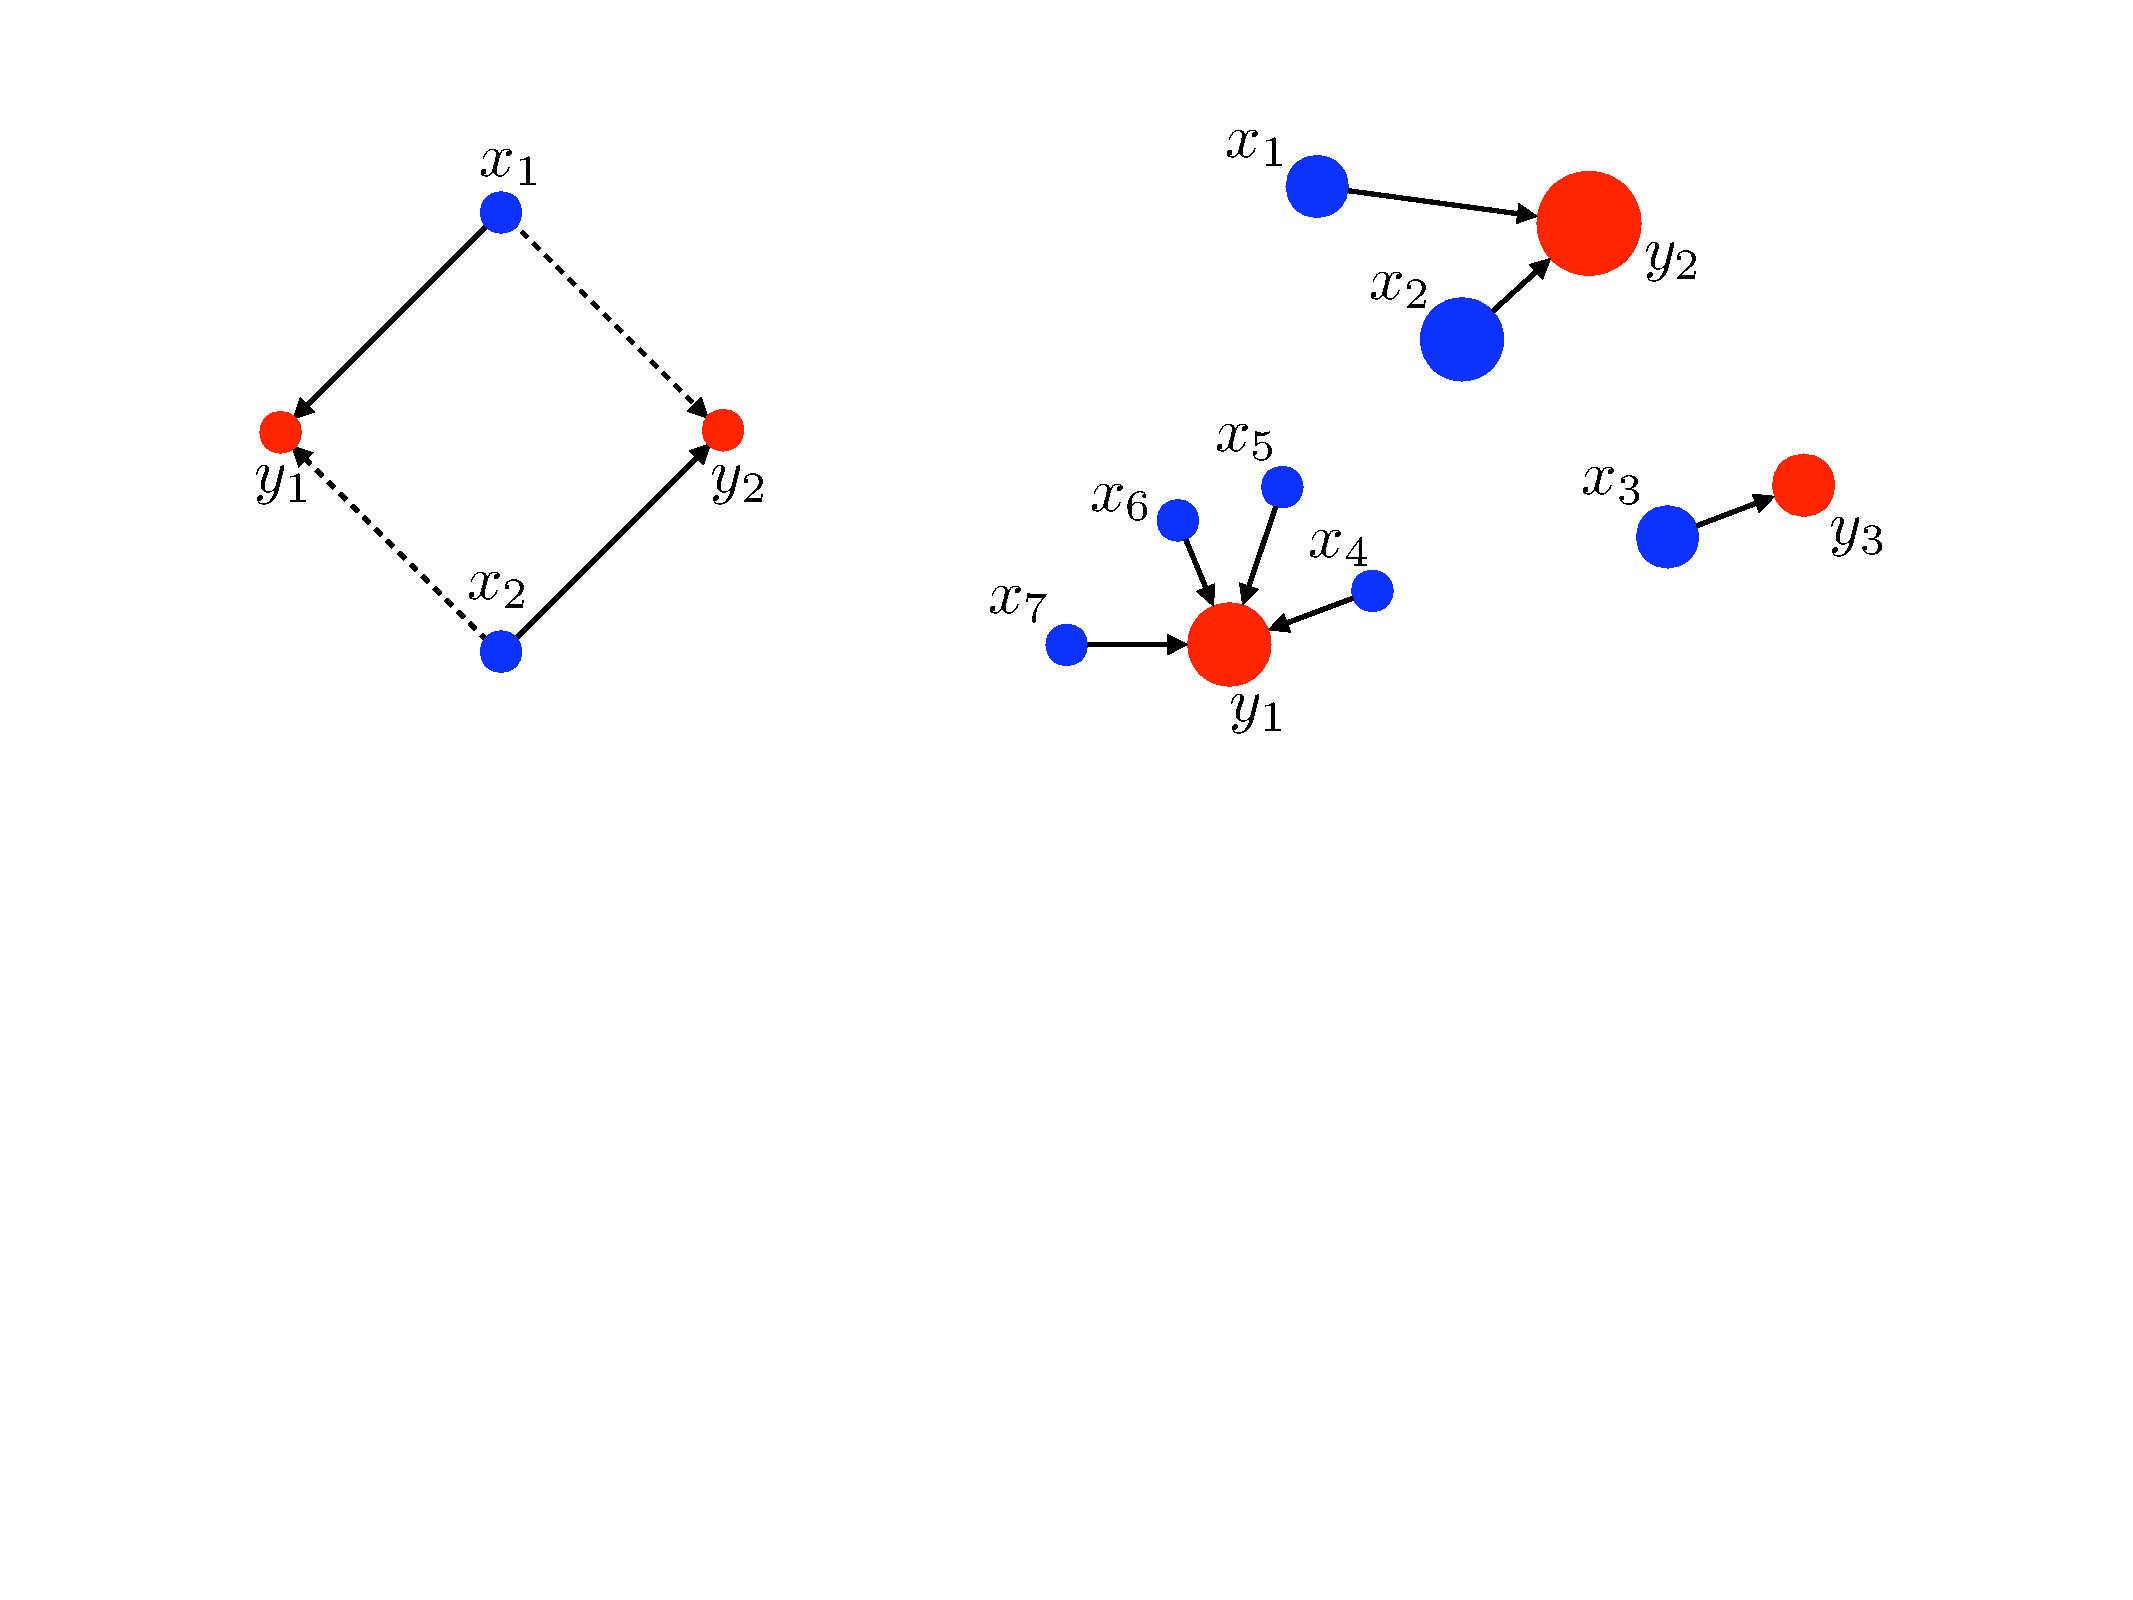
\includegraphics[width=\textwidth]{./images/non-unique-optimal-matching.pdf}
	\caption{\textit{Left}: blue dots from measure $\mu$ and red dots from measure $\nu$. The dots are pairwise equidistant. Hence, either matching $\sigma = (1, 2)$ or $\sigma = (2, 1)$ is optimal.\\ 
		\textit{Right}: a map $T$ can associate measure $\alpha$ to measure $\beta$, with weights proportional to the area of the disk. The mapping is as follows: $T(x_1) = T(x_2) = y_2, T(x_3) = y_3$ and $T(x_4) = T(x_5) = T(x_6) = T(x_7) = x_1$. However, there is no surjective $T$ from $\beta$ to $\alpha$. \\
		Figure 2.2 from \citet{peyre2020}.}
	\label{fig:unique}
\end{figure}

Consider the following OT problem:
\begin{equation}
	\min_{\pi \in \Pi(\alpha, \beta)} \sum_{i = 1}^m \sum_{j = 1}^n c_{ij} \pi_{ij},
	\label{eq:linprog}
\end{equation}
with $\Pi(a,b)$ the set of couplings on $(\alpha, \beta)$ and $c$ a given cost function. One can rewrite equation~\eqref{eq:linprog} into a standard form. Let $\mathbbm{1}_{m \times m}$ be the $m\times m$ identity matrix and let $a \otimes b$ be the Kronecker product. Then, the $(m+n) \times mn$ matrix 
\begin{equation*}
	A = \left[\begin{array}{c}
		\mathbbm{1}_{m \times m}^\top \otimes \mathbbm{1}_{n \times n} \\
		 \mathbbm{1}_{m \times m} \otimes \mathbbm{1}_{n \times n}^\top
	\end{array}\right]
\end{equation*}
can be used to encode the constraints: consider a matrix $P \in \R^{m \times n}$. One can flatten the matrix $P$ onto a vector $p \in \R^{mn}$ by writing $p_{i + m (j-1)} = P_{ij}$. Then, one has \citep{peyre2020}:
\begin{equation*}
	P \in \R^{m \times n} \in \Pi(\mu, \nu) \quad  \Leftrightarrow  \quad p\in \R_{\geq 0}^{mn}, \;\; Ap = \left[\begin{array}{c}
		\mu \\
		\nu
	\end{array}\right].
\end{equation*}
Hence, the original transport problem can be written as 
\begin{align*}
	\min_{p \in \R_{\geq 0}^{mn}} \; c^\top p, \quad \text{such that } Ap = \left[\begin{array}{c}
		\mu \\
		\nu
	\end{array}\right].
\end{align*}
However, note that $p \in \R^{mn}$, so we have $N = mn$ variables. Furthermore, $A$ is a $(m + n) \times mn$ matrix, so we have $K = m + n$ equality constraints. In general, linear programs have a complexity of $\mathcal{O}(N^2K)$ \citep{vanderbei2020}, which is cubic complexity. This can cause issues for large values of $m$ and $n$. 

\section{Entropy Regularization}
\label{sec:entropyreg}
To solve the computational difficulties in OT, \citet{cuturi2013} proposed an entropy regularization of OT. His approach smoothed the classical OT problem with an entropic term, given by
\begin{equation}
	\pi = \argmin_{\pi \in \Pi (\mu, \nu)} \left\{\langle c, \pi \rangle - \varepsilon H(\pi) \right\},
	\label{eq:eotcuturi}
\end{equation}
with $\varepsilon > 0$, $\Pi(\mu, \nu)$ the set of all couplings between $\mu$ and $\nu$, $\langle c, \pi\rangle$ the inner product between $c$ and $\pi$, and 
\begin{equation}
	H(\pi) := -\sum_i \sum_j \pi_{ij} \log \pi_{ij}
	\label{eq:entropyH}
\end{equation}
the entropy of $\pi$, with $\pi$ having entries $\pi_{ij}$. We use the convention $H(\pi) = -\infty$ if one of the entries of $\pi$ is $0$ or negative. The entropy regularized OT solves for the optimal coupling $\pi$ that minimizes the (entropy regularized) cost of transfer from $X$ to $Y$. \par
Note that for $\pi$ a probability matrix, $H$ is strongly concave: $\del^2 H(\pi) = -\text{diag}(1/\pi_{ij})$ and $\pi_{ij} \leq 1$. Therefore, the entropy-regularized problem has a unique solution. \par 
Figure~\ref{fig:impactepsilon} shows the effect of the entropy regularization on the simplex $\Sigma^3$, visualized as a triangle. Note how the entropy term pushes the original linear program solution away from the boundary of the triangle. \par 
\begin{figure}[h!]
	\centering
	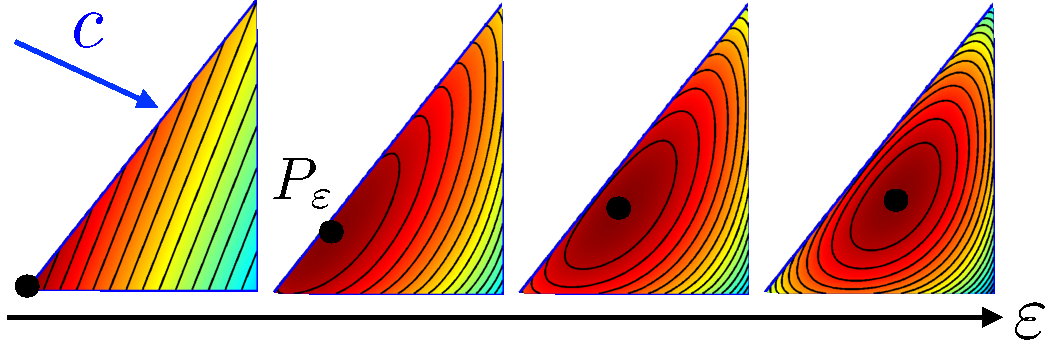
\includegraphics[width=.7\linewidth]{./images/simplex.pdf}
	\caption{Impact of $\varepsilon$ on the optimization of a linear function on the simplex $\Sigma^3$, solving equation~\eqref{eq:eotcuturi} for a varying $\varepsilon$. Figure 4.1 from \citet{peyre2020}. }
	\label{fig:impactepsilon}
\end{figure}
Entropy regularizing OT is helpful, because it takes into account the uncertainty and incompleteness of the data, and it is faster then regular OT. Furthermore, for $\varepsilon \ra 0$, the entropy regularized OT will converge to the regular OT. For $\varepsilon \ra \infty$, the solution converges to the coupling with maximal entropy between the two marginals $\mu$ and $\nu$, $\mu \nu^\top$ \citep{peyre2020}. Thus, as $\varepsilon$ increases, we have faster computational algorithms and statistical convergence. 
	
\subsection{Sinkhorn Scaling}
\label{sec:sinkhorn}
Now, let us look at a specific algorithm for solving equation~\eqref{eq:eotcuturi}. We can define the Kullback-Leibner (KL) divergence between two couplings $\pi$ and $\pihat$ as follows:
\begin{equation}
	\text{KL}(\pihat, \pi) := \sum_{i,j} \pihat_{ij} \log\left(\f{\pihat_{ij}}{\pi_{ij}}\right).
	\label{eq:KLdef}
\end{equation}
Then, the (unique) solution of \eqref{eq:eotcuturi} is a projection onto $\Pi(\mu, \nu)$ of the Gibbs kernel associated to the cost matrix $c$ as 
\begin{equation}
	K_{ij} := \exp\left(-c_{ij}/\varepsilon\right). 
	\label{eq:Kdef}
\end{equation}
After all, when combining \eqref{eq:entropyH} with \eqref{eq:eotcuturi} and using $c_{ij}/\varepsilon = -\log K_{ij}$ from \eqref{eq:Kdef} we get
\begin{align*}
	\min_{\pi \in \Pi(\mu, \nu)}  &\sum_{i,j} \pi_{ij} c_{ij}  + \varepsilon \sum_{ij} \pi_{ij} \log \pi_{ij} \\
	= &\min_{\pi \in \Pi(\mu, \nu)}  \sum_{i,j} \f{\pi_{ij} c_{ij}}{\varepsilon} + \sum_{ij} \pi_{ij} \log \pi_{ij} \\
	= &\min_{\pi \in \Pi(\mu, \nu)} -\sum_{i,j} \pi_{ij} \log K_{ij}  + \sum_{ij} \pi_{ij} \log \pi_{ij} \\
	= &\min_{\pi \in \Pi(\mu, \nu)}  \sum_{i,j} \pi_{ij} \log \f{\pi_{ij}}{K_{ij}}  \\
	= &\;  KL(\pi, K).
\end{align*}
\vspace{0.3cm}
\begin{proposition}
	The solution to \eqref{eq:eotcuturi} is unique and has the form 
	\begin{equation}
		\pi_{ij} = u_i K_{ij} v_j,
		\label{eq:propbenamou}
	\end{equation}
	for $1 \leq i \leq m, 1 \leq j \leq n$ and two scaling variables $u \in \R^m_{\geq 0}, v \in \R^n_{\geq 0}$. 
\end{proposition}
The proof can be found in \citet{peyre2020}, proposition 4.3. \par 
Note that equation~\eqref{eq:propbenamou} can be rewritten as $\pi = \text{diag}(u) K \text{diag}(v)$. Therefore, there must hold 
\begin{equation}
	\text{diag}(u)K\text{diag}(v) \mathbbm{1}_n = \mu \;\;\; \text{and} \;\;\; \text{diag}(v) K^\top \text{diag}(u) \mathbbm{1}_m = \nu.
	\label{eq:ukvdiag}
\end{equation}
Now, note that $\text{diag}(v) \mathbbm{1}_n = v$ and $\text{diag}(u) \mathbbm{1}_m = u$, thus we can see that this is equivalent to 
\begin{equation}
	u \circledast (Kv) = \mu \;\;\;\text{and}\;\;\; v \circledast (K^\top u) = \nu,
	\label{eq:sinkhorn}
\end{equation}
with $\circledast$ the entry-wise multiplication of vectors. This problem is known as the matrix scaling problem \citep{nemirovski1999}. \par 
One way to solve this problem is by Sinkhorn's algorithm \citep{sinkhorn1964}, which can be seen in Algorithm~\ref{alg:sinkhorn}. First we modify $u$ so that it satisfies the left hand side of \eqref{eq:sinkhorn} and then modify $v$ so that it satisfies the right hand side. The updates are then given by 
\begin{equation}
	u^{(l + 1)} := \f{\mu}{Kv^{(l)}} \;\;\; \text{and} \;\;\; v^{(l+1)} := \f{\nu}{K^\top u^{(l+1)}},
\end{equation}
initialized by some arbitrary vector $v^{(0)} \in \R^n$. We stop the iterations when the Euclidean distance $||\cdot||^2$ between the updates of $u$ and $v$ is smaller than some convergence limit $k_u$ and $k_v$ respectively. 
\vspace{0.3cm}
\begin{remark}
	A different initialization will likely end with a different $u$ and $v$, as they are only defined up to a multiplicative constant: if $u$ and $v$ satisfy \eqref{eq:ukvdiag}, then $\lambda u$ and $v/\lambda$ also satisfy \eqref{eq:ukvdiag}, for any $\lambda > 0$. However, these iterations will converge and lead to the same optimal coupling \citep{peyre2020}. Furthermore, note that Algorithm~\ref{alg:sinkhorn} is always convergent for large enough $\varepsilon$. 
\end{remark}
\begin{algorithm}[b]
	\caption{Sinkhorn's Algorithm for OT}
	\textbf{Input: } Cost matrix $c \in \R^{m \times n}$ and regularization parameter $\varepsilon > 0$ and marginals $\mu \in \R^m, \nu \in \R^n$. \\
	\textbf{Initialize:} $v = (1/n, \dots, 1/n) \in \mathbb{R}^{n}$ and $K = \exp(c/\varepsilon)$ \\
	\Repeat{\text{convergent: $||u^{(l)} - u^{(l+1)}||^2 < k_u$ and $||v^{(l)} - v^{(l+1)}||^2 < k_v$}}{
		$u \leftarrow \mu / (K v)$\;
		$v \leftarrow \nu / (K^\top u)$\;
	}
	\KwOut{$\pihat = uKv$}
	\label{alg:sinkhorn}
\end{algorithm}

\vspace{0.3cm}
\begin{example}[Sinkhorn's Algorithm]
	Consider $X = \{x_1, x_2\} = \{1, 3\}$ and $Y = \{y_1, y_2\} = \{2, 4\}$ and two observed probabilities $\mu = (\mu_1, \mu_2) = (1/3, 2/3)$ and $\nu = (\nu_1, \nu_2)= (2/3, 1/3)$. Assume we are given a cost function $c(x,y) = ||x-y||^2$, with $||\cdot||^2$ the Euclidean distance. Then, we can see for the cost matrix:
	\[c = \left(\begin{array}{cc}
		(1-2)^2 & (1-4)^2 \\ 
		(3-2)^2 & (3-4)^2
	\end{array}\right) = \left(\begin{array}{cc}
		1 & 9 \\ 
		1 & 1
	\end{array}\right). \]
	Now, let us investigate Sinkhorn's algorithm. Initialize $v^{0} = (1/2, 1/2)$ and choose $\varepsilon = 0.1$. We can see 
	\[K = e^{-c/\varepsilon} = \left(\begin{array}{cc}
		e^{-1/0.1} & e^{-9/0.1} \\ 
		e^{-1/0.1} & e^{-1/0.1}
	\end{array}\right) \approx \left(\begin{array}{cc}
		4.5 \cdot 10^{-5} & 8.2\cdot 10^{-40} \\ 
		4.5 \cdot 10^{-5} & 4.5 \cdot 10^{-5}
	\end{array}\right).  \]  
	Let us now look at the first iteration: 
	\[u^{(1)} = \f{\mu}{Kv^{(0)}} = \left(\begin{array}{c}
		14684.3 \\ 14684.3 
	\end{array}\right), \quad \text{ and }\quad v^{(1)} := \f{\nu}{K^\top u^{(1)}} = \left(\begin{array}{c}
		0.5 \\ 0.5
	\end{array}\right). \]
	Let us also calculate the second iteration: 
	\[u^{(2)} = \f{\mu}{Kv^{(1)}} = \left(\begin{array}{c}
		14684.3 \\ 14684.3 
	\end{array}\right), \text{ and } v^{(2)} := \f{\nu}{K^\top u^{(2)}} = \left(\begin{array}{c}
		0.5 \\ 0.5
	\end{array}\right). \]
	If we calculate the Frobenius norm, $||\cdot||_F$ of these two iterations, we can see 
	\[ ||u^{(2)} - u^{(1)}||_F \approx 0, \text{ and } ||v^{(2)} - v^{(1)}||_F \approx 0. \]
	This is a very small deviation, and indeed, if we calculate even more iterations, we can see that difference between $u^{(l)}$ and $u^{(l+1)}$ and the difference between $v^{(l)}$ and $v^{(l+1)}$ gets smaller and smaller, thus the algorithm is converging.\par 
	At iteration 20, the difference in $u$ stays down at $0$, as well as the difference in $v$. Calculating the transportation matrix $\pihat$ from this, we get 
	\[ \pihat = u_i v_j K_{ij} \approx \left(\begin{array}{cc}
		0.33 & 6.02 \cdot 10^{-36} \\
		0.33 & 0.33
	\end{array}\right) .  \]
\end{example}

\section{Inverse Optimal Transport}
In some cases, you already know the transportation matrix $\pi$, but you do not know the cost matrix $c$ yet. This case, where you want to solve for $c$, is called \textit{inverse Optimal Transport}, or iOT; it studies the problem of inferring the underlying cost matrix given an observation on coupling two probability measures, such as in transportation. \par 
To solve for the cost function, we will first need to define iOT. However, unlike for the forward problem \citep{villani2008}, the mathematical foundations of the inverse problem have not been intensively studied. Some of the main contributions on iOT are applications of internal migration \citep{stuart2020}, estimating marriage matching \citep{ma2021}, the problem of iOT with noisy and incomplete matching data \citep{li2019}, and the definition on discrete probabilistic iOT \citep{chiu2022}. \par 
To define iOT, let us look at two measurable spaces $X = \{x_1, \dots, x_m\}$ and $Y = \{y_1, \dots, y_n\}$, with $m, n \geq 2$, as the cases where $m=1$ or $n=1$ are trivial. Let $\pi = (\pi_{ij})_{m \times n} \in \R_{\geq 0}^{m \times n}$ be a coupling. Here, $\pi_{ij}$ represents the probability of observing $x_i$ and $y_j$ simultaneously. This interaction can be obtained by a cost matrix $c = (c_{ij})_{m \times n} \in (\R_{\geq 0} \cup \{\infty\})^{m \times n}$, with $c_{ij}$ being the cost of coupling $x_i$ and $y_j$, just as in the forward problem. \par 
Now, given a coupling $\pi$, the inference on $c$ can be formulated as an inverse entropy regularized OT. We know that entropy regularized OT is the map 
\[\Phi: (\R_{\geq 0} \cup \{\infty\})^{m \times n} \times \mathcal{P}(\R^m) \times \mathcal{P}(\R^n) \ra \mathcal{P} (\R_{\geq 0}^{m \times n}), \]
with $\Phi(c, \mu, \nu) = \pi$, $\pi$ as in \eqref{eq:eotcuturi} and $\mathcal{P}(X)$ the set of probability measures on $X$. Then, the inverse entropy regularized OT can be defined as $\Phi^{-1}: \pi \ra \{(c, \mu, \nu)\}$, with $\{(c, \mu, \nu)\}$ the pre-image set of $\pi$ under $\Phi$. 
\vspace{0.3cm}
\begin{remark}
	If $\pi$ is observed without any noise, it completely determines $\mu$ and $\nu$: from $(c, \mu, \nu) \in \Phi^{-1}(\pi)$, we know $\pi \in \Pi(\mu, \nu)$, thus $\mu$ and $\nu$ are the marginals of $\pi$. Thus, we can reduce the problem into $\Phi^{-1}: \pi \ra \{c\}$. However, $\Phi^{-1}: \pi \ra \{c\}$ is not a well-defined function, since $\pi$ does not uniquely determine $c$; for example two cost matrices may differ by an additive constant. 
\end{remark}
Note that we are looking at the entropy regularized OT instead of the regular OT, since the transportation matrix $\pihat$ is in general sparse, and zero elements do not carry enough information to say something meaningful about the cost: a zero in $\pihat$ does not necessarily mean that the underlying cost is infinite \citep{chiu2022}. 






\chapter{Data}
\label{ch:data}

\section{FLAMINGO}
The main data used is the FLAMINGO (Full-hydro Large-scale structure simulations with All-sky Mapping for the Interpretation of Next Generation Observations) simulations, see also \citet{schaye2023, kugel2023}. The FLAMINGO simulations are large-scale hydrodynamical simulations, that explicitly incorporate baryonic physics. The aim of these simulations is to provide more accurate theoretical predictions for observational cosmology, particularly on smaller scales where baryonic effects become more dominant and complex. \par 
The FLAMINGO data we used contains an initial distribution of particles, and eight subsequent evolutionary timestamps. In general, information includes the scale factor and redshifts. Then, for each timestamp, information about the particle locations, types and masses are given. \par 
We used a dark-matter only simulation, with a box size of $400$ Mpc and $360^3$ particles. A projection of the cold dark matter surface density can be found in Figure~\ref{fig:cdmdensity}. Some denser and less-dense structures can be seen, as we would expect in the Cosmic Web. The data was processed with \lstinline|swiftsimio| \citep{swiftsimio}. Besides the FLAMINGO data, we have generated data for specific patterns of motion, which will be elaborated in Chapter~\ref{ch:results}. 

\begin{figure}[!ht]
	\centering 
	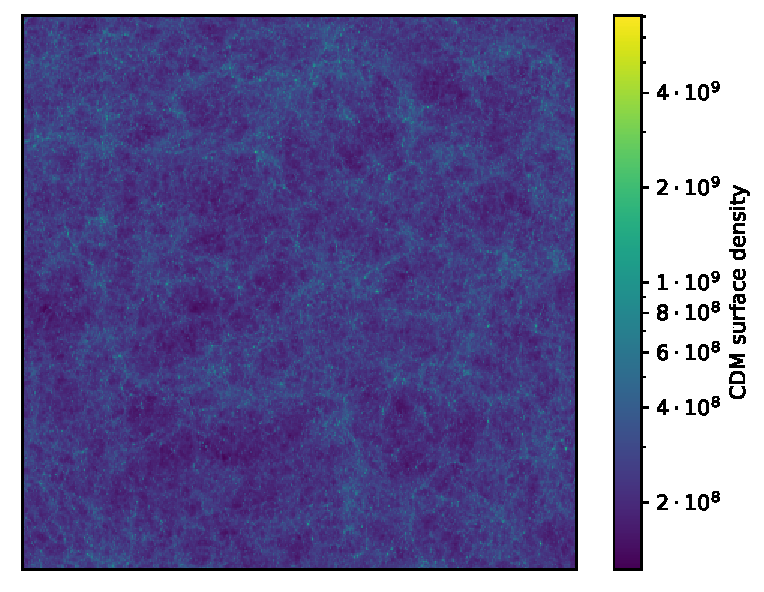
\includegraphics[width=8cm]{./images/projection.pdf}
	\caption{Cold Dark Matter (CDM) surface density of the used FLAMINGO simulation; a dark-matter only simulation with a box size of $400$ Mpc and $360^3$ particles.}
	\label{fig:cdmdensity}
\end{figure}

\subsection{Boxes}
\label{sec:boxes}
As the simulations have about 50 million particles for each time-step, evaluating each particle can be computationally expensive. To not look into each particle separately, the data is divided into $n^3$ boxes of equal size - each axis is divided into $n$ parts. The boxes are counted in the following way: box $0$ is the box around $(0, 0, 0)$. Then, taking the same $x$ and $y$, we will count the boxes upward in $z$. Once we have reached the maximum $z$-value, we will move up one $y$-segment, and again count up in $z$. We repeat this until there are no more $y$-segments. Once this is the case, we move up one $x$-segment, and repeat this process. We stop once all the $x$-values have been covered, resulting in $n^3$ boxes. The $n=2$ case can be seen in Figure~\ref{fig:boxes}. Note that we implicitly assume here, that there are no negative coordinates. \par %This is always the case in the simulations always the case, and other situations can always be translated into this case. \par
\begin{figure}[!ht]
	\centering
	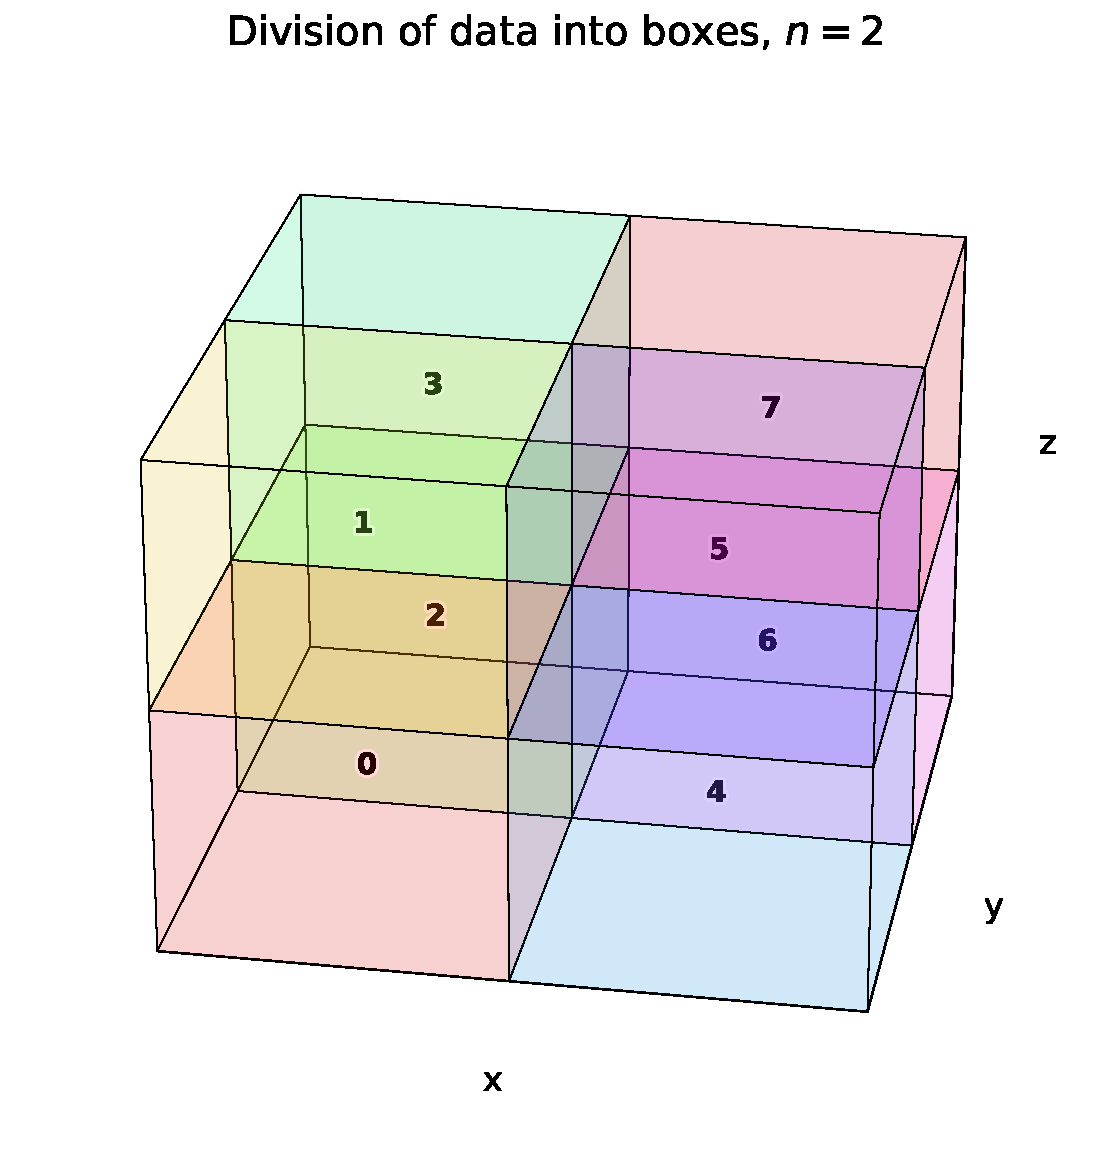
\includegraphics[width=8cm]{./images/boxes.pdf}
	\caption{Division of the data into boxes, for the case $n=2$. }
	\label{fig:boxes}
\end{figure}


By dividing the data into boxes, the cost matrix will be a function of these boxes, and not of the specific particles. Therefore, the cost matrix depends on the amount of particles in each box and the dynamics of those particles on average, rather then the dynamics of the individual particles. 





\chapter[Algorithm for Inverse Optimal Transport]{Algorithm for Inverse \\Optimal Transport}
\label{ch:entropyregiOT}
Our objective is to find the cost matrix of the observed transport in our data. To find the cost matrix, we will use an algorithm inspired by \citet{ma2021}. We will follow part of their derivation, while discretizing some steps along the way. As we are working in a discrete case, all our input and output variables will be vectors and matrices. Let $n \in \Z_{\geq 1}$ be the number of points or, in our case, the number of boxes as described in Section~\ref{sec:boxes}. Our input and output spaces are the same space, $X \subseteq \R^m$ and $Y \subseteq \R^{n}$, with $m=n$. However, we will keep $m$ and $n$ separate for clarification in the derivations. Then, $\mu \in \Delta^{m-1}, \nu \in \Delta^{n-1}$ are probability vectors, with $\Delta^{n-1}:=\left\{x=\left(x_{1}, \ldots, x_{n}\right) \in\right.$ $\left.\mathbb{R}^{n}: x_{i} \geq 0, \sum_{i=1}^{n} x_{i}=1\right\}$ the standard probability simplex in $\mathbb{R}^{n}$, and $\pi, c \in \R^{m \times n}$. Note that $\mu$ and $\nu$ are (discrete) measures, but we can view them as vectors as we can assume all our data points are distinct and fixed with the same weight. With this notation, equation~\eqref{eq:eotcuturi} can be written as
\begin{equation}
	\min _{\pi \in \mathbb{R}^{m \times n}}\left\{\langle c, \pi\rangle: \pi \geq 0, \pi \mathbbm{1}_{n}=\mu, \pi^{\top} \mathbbm{1}_{m}=\nu\right\},
	\label{eq:cpi}
\end{equation}
with $\langle c, \pi\rangle =\sum_{i, j} c_{i j} \pi_{i j}$ the inner product and $\mathbbm{1}_{n}:=(1, \ldots, 1)^{\top} \in \mathbb{R}^{n}$, as before. \par 
A modification of equation~\eqref{eq:cpi} was proposed by \citet{cuturi2013}, with an additional entropy regularization term in the objective function, as in Section~\ref{sec:entropyreg}:
\begin{equation}
	\min _{\pi \in \mathbb{R}^{m \times n}}\left\{\langle c, \pi\rangle-\varepsilon H(\pi): \pi \mathbbm{1}_{n}=\mu, \pi^{\top} \mathbbm{1}_{m}=\nu\right\},
	\label{eq:entropy}
\end{equation}
where $H(\pi):=-\langle\pi, \log \pi\rangle=-\sum_{i, j} \pi_{i j}\left(\log \pi_{i j}\right)$ is the Shannon entropy of $\pi$, as in equation~\eqref{eq:entropyH}, and $\varepsilon>0$ is the weight of the entropy regularization. Note that there are different definitions of $H$, some have an extra term $-1$. However, this extra term does not matter for our purposes, as long as we are consistent with our definition of $H$. Due to the entropy term in \eqref{eq:entropy}, the inequality constraint in equation~\eqref{eq:cpi} is eliminated. Furthermore, the objective function in equation~\eqref{eq:entropy} becomes strictly convex, therefore having a unique solution \citep{ma2021}. \par 
For the rest of this chapter, let us write $c$ for the theoretical cost matrix, $c^*$ for the actual cost matrix and $\chat$ for the cost matrix as retrieved from an algorithm.

\section{The Dual Formulation of Inverse Optimal Transport}
Now, let $\Pi(\mu, \nu)$ be the set of probability measures $\pi \in P(X \times Y)$ such that $\pi(A \times Y) = \mu(A)$ and $\pi(X \times B) = \nu(B)$, for any measurable set $A \subseteq X, B \subseteq Y$. Thus $\mu_i = \sum_j \pi_{ij}$ and $\nu_j = \sum_i \pi_{ij}$. Let $\alpha \in \R^m$ and $\beta \in \R^n$ be the Lagrangian multipliers corresponding to the marginal constraints. We can then rewrite equation~\eqref{eq:entropy} as 
\begin{equation}
	\min _{\pi \in \Pi(\mu, \nu)}\left\{\langle c, \pi\rangle-\varepsilon H(\pi)\right\}.
	\label{eq:entropynew}
\end{equation}
Now, the dual problem of equation~\eqref{eq:entropynew} can be calculated. 
\vspace{0.3cm}
\begin{lemma}
	The dual problem of \eqref{eq:entropynew} is given by 
	\begin{equation}
		D(\alpha, \beta) := \sum_{i=1}^m \alpha_i \mu_i + \sum_{j=1}^n \beta_j \nu_j - \varepsilon \sum_{i=1}^m \sum_{j=1}^n \exp\left(\frac{\alpha_i + \beta_j - c_{ij} - \varepsilon}{\varepsilon}\right),
		\label{eq:Dinproof}
	\end{equation}
	and the dual optimization problem is given by 
	\begin{equation}
		\max_{\alpha \in \R^m, \beta\in \R^n} D(\alpha, \beta).
		\label{eq:dual}
	\end{equation}
	\label{lemma:dual}
\end{lemma}
The proof of this lemma can be found in Appendix~\ref{sec:prooflemmadual}. \par 
Let $(\alpha^*, \beta^*)$ be the optimal solution for the dual problem. Note that from the proof of Lemma~\ref{lemma:dual}, equation~\eqref{eq:rhodef} holds:
\begin{equation}
	\pi_{ij}^* = \exp\left[\f{\alpha_i^* + \beta_j^* - c^*_{ij} - \varepsilon}{\varepsilon}\right] .
	\label{eq:pi}
\end{equation}
Now, let us consider the inverse problem: suppose we are given $\mu \in \R^m$, $\nu \in \R^n$ and $\pi^* \in \R^{m \times n}$. We then want to retrieve the cost matrix $\chat \in \R^{m \times n}$. \citep{ma2021} proposed an iOT to find $\chat$, which is, in the discretized form:
\begin{subequations}
	\begin{equation}
		\chat = \min_c\; \text{KL}(\pi^*, \pi^c) + \varepsilon^{-1} R(c),  \label{eq:KLa}
	\end{equation}
	\begin{equation}
		\text{such that } \pi^c = \argmin_{\pi \in \R^{m \times n}} \left\{\sum_{i,j} c_{ij} \pi_{ij} - \varepsilon H(\pi) \right\}. \label{eq:KLb}
	\end{equation}
	\label{eq:KL}
\end{subequations}
Here, KL$(\pi^*, \pi^c)$ is the (discrete) Kullback-Leibler (KL) divergence between $\pi^*$ and $\pi^c$, as in equation~\eqref{eq:KLdef} and $R(c)$ the regularization on $c$, which will be described more in Section \ref{sec:rc}. In essence, equations~\eqref{eq:KLa} and \eqref{eq:KLb} adjust $\chat$ so that the theoretical $\pi^c$, the optimal transport plan induced by $c$, is as close to the empirical $\pi^*$ as possible, measured by the KL distance. \par 
Note that the optimization problem in equations~\eqref{eq:KLa} and \eqref{eq:KLb} is a bi-level optimization problem, which is usually quite computationally heavy. However, we can prove it is equivalent to an unconstrained problem in $c$, by using the dual form \eqref{eq:dual}. 
\vspace{0.3cm}
\begin{theorem}
	The optimization problem in equations~\eqref{eq:KLa} and \eqref{eq:KLb} is equivalent to 
	\begin{equation}
		\min _{\alpha \in \R^m, \beta \in \R^n, c\in \R^{m \times n}} E(\alpha, \beta, c)+R(c), 
		\label{eq:10}
	\end{equation}
	with 
	\begin{equation}
		E(\alpha, \beta, c) := \sum_{i,j} c_{ij} \pihat_{ij} - \sum_i \alpha_i \mu_i - \sum_j \beta_j \nu_j + \varepsilon \sum_{i,j} e^{(\alpha_i + \beta_j - c_{ij}-\varepsilon)/\varepsilon}.
		\label{eq:E}
	\end{equation}
	Here, equivalent means that $c^*$ solves \eqref{eq:KL} if and only if $(\alpha^{c^*}, \beta^{c^*}, c^*)$ solves \eqref{eq:10} with $(\alpha^{c^*}, \beta^{c^*})$ the optimal solution for the dual problem~\eqref{eq:dual} with cost $c^*$.
	\label{thm:2}
\end{theorem}
The proof can be found in Appendix~\ref{sec:proofthm2}.


\subsection{Equivalence of Solutions}
The possibility of solving \eqref{eq:10} more efficiently than \eqref{eq:KL}, comes from the fact that $E$ is a jointly convex functional on 
\[\W := \R^m \times \R^n \times \R^{m \times n}.\]
Note, however, that $E$ is not strictly convex in $(\alpha, \beta, c)$, so we cannot claim uniqueness of the minimizer - there are actually infinitely many solutions of \eqref{eq:10} with the same $\pihat$, if there is no additional constraint $R$ \citep{ma2021}. However, we can see that the optimal solution set is given by an equivalence class of some equivalence relation. \par 
\vspace{0.3cm}
\begin{definition}
	$(\alpha, \beta, c)$ and $(\bar{\alpha}, \bar{\beta}, \bar{c})$ are \textbf{equivalent}, $(\alpha, \beta, c) \sim (\bar{\alpha}, \bar{\beta}, \bar{c})$, if $\alpha_i + \beta_j - c_{ij} = \bar{\alpha}_i+ \bar{\beta}_j - \bar{c}_{ij}$ for all $1 \leq i \leq m, 1 \leq j \leq n$. 
	\label{def:equivalence}
\end{definition}
It is easy to see that $\sim$ is an equivalence relation over $\W$. We will omit the proof for conciseness. The equivalence relation in Definition~\ref{def:equivalence} induces a quotient space $\widetilde{\W} := \W /\sim$. Let $[(\alpha, \beta, c)] \subseteq \widetilde{\W}$ be the equivalence class of $(\alpha, \beta, c)$. Then, there holds the following for $E$: 
\vspace{0.3cm}
\begin{theorem}
	The following statements are true for $E(\alpha, \beta, c)$ in \eqref{eq:10}:
	\begin{enumerate}[label=(\roman*)]
		\item $E(\alpha, \beta, c)$ is jointly convex in $(\alpha, \beta, c)$;
		\item $E$ is a constant on the equivalence class $[(\alpha, \beta, c)]$ for each $(\alpha, \beta, c) \in \W$; 
		\item The functional $\widetilde{E}: \widetilde{\W} \ra \R$ with $\widetilde{E}([(\alpha, \beta, c)]) = E(\alpha, \beta, c)$ is well defined;
		\item If $(\alpha^*, \beta^*, c^*)$ is a solution of \eqref{eq:10}, then the optimal transport plan $\pi^*$ in \eqref{eq:KL} is given by 
		\[\pi^*_{ij} = e^{(\alpha^*_i + \beta^*_j - c^*_{ij}-\varepsilon)/\varepsilon};\]
		\item $[(\alpha^*, \beta^*, c^*)]$ as in $(iv)$ is the unique minimizer of $\widetilde{E}$. 
	\end{enumerate}
	\label{thm:3}
\end{theorem}
The proof can be found in Appendix~\ref{sec:proofthm3}. \par 
From Theorem~\ref{thm:3} we can see that \eqref{eq:10} is convex as long as $R$ is convex, or imposes constraints on a convex set. But even without knowledge of a specific $R$, we can characterize the entire optimal solution set, by finding one minimizer of $E$ and making use of the equivalence relation. 

\section{Algorithm Development}
As we have seen, $\pi$ is a real-valued $m \times n$ matrix. In our case, we can divide the data into boxes, as described in Section~\ref{sec:boxes}, and define
\[ \hat{\pi}_{i j} :=\frac{N_{i j}}{N}, \]
with $N_{i j}$ the number of particles going from box $i$ to box $j$, and $N=\sum_{i, j} N_{i j}$. Then, we have the following optimization problem of equation~\eqref{eq:10}:
\begin{equation}
	\min _{\alpha\in \R^m, \beta\in\R^n, \chat\in\R^{m\times n}}\{R(\chat)-\langle\alpha, \mu\rangle-\langle\beta, \nu\rangle+\langle \chat, \hat{\pi}\rangle+s(\alpha, \beta,\chat)\} ,
	\label{eq:10discrete}
\end{equation}
with $s: \mathbb{R}^{m} \times \mathbb{R}^{n} \times \R^{m \times n} \rightarrow \mathbb{R}$ given as
\begin{equation}
	s(\alpha, \beta, \chat):=\varepsilon \sum_{i, j} e^{\left(\alpha_{i}+\beta_{j}-\chat_{i j}-\varepsilon\right) / \varepsilon}=\varepsilon\left\langle e^{\left(\alpha_{i}+\beta_{j}-\chat_{i j}-\varepsilon\right) / \varepsilon}, 1\right\rangle .
	\label{eq:s}
\end{equation}
To solve \eqref{eq:10discrete}, we can use a update scheme also known as Block Coordinate Descent (BCD). In general, BCD requires joint convexity of $E$, which is shown to be true in Theorem~\ref{thm:3}, and Lipschitz continuity of its gradient \citep{beck2015}, which is not true in our case. There is, however, an alternative formulation which is equivalent to the minimization in equation~\eqref{eq:10}, where the objective function does have a Lipschitz continuous gradient.
\vspace{0.3cm}
\begin{lemma}
	The inverse Optimal Transport minimization \eqref{eq:10} has the same set of solutions as the following minimization:
	\begin{equation}
		\min _{\alpha, \beta, c} \Psi(\alpha, \beta, c):=F(\alpha, \beta, c)+R(c) ,
		\label{eq:lemma}
	\end{equation}
	with
	\[ F(\alpha, \beta, c)=-\langle\alpha, \mu\rangle-\langle\beta, \nu\rangle+\langle c, \hat{\pi}\rangle+\varepsilon \log \left(\left\langle e^{\left(\alpha_{i}+\beta_{j}-c_{i j}-\varepsilon\right) / \varepsilon}, 1\right\rangle\right) .\]
	\label{lemma:inverseOT}
\end{lemma}
The proof of this lemma can be found in Appendix~\ref{sec:prooflemmainverseOT}. \par 
At this point, we can consider our Algorithm \ref{alg:1}. We know that given $c$, the optimal coupling $\pihat$ between $\mu$ and $\nu$ as in \eqref{eq:eotcuturi} can be solved by applying $(\mu, \nu)$-Sinkhorn scaling on $K = e^{-\chat/\varepsilon}$, as in Section~\ref{sec:sinkhorn}. \citet{ma2021} advocated for a modified algorithm to the standard BCD, with similar updates for $\alpha$ and $\beta$, but a modification for the update of $\chat$ by splitting it into multiple steps for the inverse problem, as can be seen in Algorithm~\ref{alg:1}. After the Sinkhorn steps, as in Algorithm~\ref{alg:sinkhorn}, we do a scaling to compute the $m\times n$ matrix $K$, with 
\begin{equation}
	K_{ij} = \f{\pihat_{ij}}{e^{(\alpha_i +\beta_j)/\varepsilon}},
	\label{eq:mawrong}
\end{equation}
for $i\in \{1, \dots, m\}, j \in \{1, \dots, n\}$. After all, $K = e^{-\chat/\varepsilon}$ and, from \eqref{eq:pi}
\[\pihat = \exp\left(\f{\alpha + \beta - \chat - \varepsilon}{\varepsilon}\right).\]
Then, you take a proximal gradient descent to obtain $\chat$: 
\begin{equation}
	\chat = \prox_{\gamma R} (-\varepsilon (\log(K) + 1)) := \argmin_{c \in \R^{m \times n}} \left\{	R(c) + \f{1}{2\gamma} ||c - \xi||^2\right\}.
	\label{eq:prox}
\end{equation}
Here, $\xi := -\varepsilon (\log(K) + 1)$, $||\cdot||^2$ is the Frobenius norm and all operations are performed component-wisely. We stop when the Euclidean distance $||\cdot||^2$ between the updates of $u$ and $v$ is smaller than some convergence limit $k_u$ and $k_v$ respectively. \par 
\vspace{0.3cm}
\begin{remark}
	Note that, since $\pihat$ only has information about the ratio $\chat/\varepsilon$, we can set $\varepsilon = 1$ without loss of generality. Then, we will recover $\chat/\varepsilon$, which is $c$ up to a constant scaling.
\end{remark}
\vspace{0.3cm}
\begin{remark}
	Notably, equation~\eqref{eq:mawrong} is different than in \citet{ma2021}, as they have obtained a transport plan that is slightly different than ours, 
		\[ \pi_{ij}^* = \exp\left[\f{\alpha_i^* + \beta_j^* - c_{ij}^*}{\varepsilon}\right]. \] 
	However, the extra $-\varepsilon$ term in our case was due to the chain rule in the proof of Lemma~\ref{lemma:dual}. This extra $\varepsilon$-term also alters the algorithm a bit from the algorithm of \citet{ma2021}. However, a constant scaling is not thought to matter, since $\alpha$ and $\beta$ are probability vectors and $\pihat$ is a probability matrix, so extra scaling will factor out with the normalization of $\alpha, \beta$ and $\pihat$. As can be seen in Appendix~\ref{sec:differencesma}, the original algorithm of \citet{ma2021} differs with a constant scaling of our algorithm, except for the $M_c$ terms, which are a result of our choice of $R$. 
	\label{rem:mawrong}
\end{remark}
\vspace{0.3cm}
\begin{algorithm}[t]
	\caption{Cost Learning Algorithm for Inverse OT}
	\textbf{Input: } Observed matrix $\hat{\pi} \in \mathbb{R}^{m \times n}$ and its marginals $\mu \in \mathbb{R}^m$, $\nu \in \mathbb{R}^n$\\
	\textbf{Initialize:} $\alpha \in \mathbb{R}^{m \times 1}$, $\beta \in \mathbb{R}^{n \times 1}$, $u = \exp(\alpha / \varepsilon)$, $v = \exp(\beta / \varepsilon)$, $\chat \in \mathbb{R}^{m \times n}$ \\
	\Repeat{\text{convergent: $||u^{(l)} - u^{(l+1)}||^2 < k_u$ and $||v^{(l)} - v^{(l+1)}||^2 < k_v$}}{
		$K \leftarrow e^{-\chat / \varepsilon}$\;
		$u \leftarrow \mu / (K v)$\;
		$v \leftarrow \nu / (K^\top u)$\;
		$K \leftarrow \hat{\pi} / (u v^\top)$\;
		$c \leftarrow \text{prox}_{\gamma R}(-\varepsilon (\log(K) + 1))$\;
	}
	\KwOut{$\alpha = \varepsilon \log u$, $\beta = \varepsilon \log v$, $\chat$}
	\label{alg:1}
\end{algorithm}


\section{Algorithm Implementation}
\label{sec:algimp}
Now, we can use Algorithm~\ref{alg:1} to find the cost matrix of multiple different scenarios. In this section, we will comment on the implementation of the algorithm, whereas the results will be described in Chapter~\ref{ch:results}. \par 
In the application of Algorithm~\ref{alg:1}, a convergence limit of $k_u = k_v = 10^{-4}$ was used. 

\subsection{Numerical Stability}
Algorithm~\ref{alg:1} is implemented in Python. For initializing $\alpha, \beta$ and $\chat$, we have chosen a random initial conditions using \lstinline|numpy|; \lstinline|alpha = np.random.rand(n)|, \lstinline|beta = np.random.rand(n)| and \lstinline|c = np.random.rand(n, n)|, with $n$ the number of boxes. For testing purposes, we also used these random initial conditions multiplied by $100$. After running the algorithm multiple times on the same dataset, we confirmed that the output of the algorithm is indeed independent of the initialization. \par 

\subsubsection{Floor}
Note that $\pihat$ can contain quite a few zeros. For example, if we consider a simulation with only collapse towards the center point, we would not expect any movement from the center point outwards, which would result in zeros in $\pihat$. Due to the fact that in Algorithm~\ref{alg:1} we set $K = \pihat/(uv^\top)$, and later divide by both $Kv$ and $K^\top u$, if $\pihat$ has zero values, we will eventually end up dividing by $0$. To solve this division problem, we manually changed the zero-values in $\mu, \nu$ and $\pihat$ to a floor value, $1/N^3$, with $N$ the number of particles. We expect this change to not have a significant influence on the generated cost matrix, because if we slightly increase the floor value, it does not change the cost matrix significantly for smaller values of $n$ (the number of boxes). However, for larger $n$, a floor-value of $1/N$ will generate unexpected patterns in the cost matrix for the reference cases. These are thought to be artefacts of the floor and go away if we decrease the floor to $1/N^3$. After changing the values of $\mu, \nu$ and $\pihat$ slightly, we re-normalize to ensure they are probability vectors. 
 
\subsection{Minimization and choosing $R(c)$}
\label{sec:rc}
At the end of the loop of Algorithm~\ref{alg:1}, we need to calculate the proximal gradient for the minimization. This proximal gradient can cause some problems, as for a larger number of boxes $n$, a standard Python minimization package, such as \lstinline|scipy.optimize.minimize|, usually creates a $n^2 \times n^2$ matrix to minimize the given expression, subsequently trying to create arrays which were too big for a personal computer. To solve these computational problems, we tried other minimization libraries, such as \lstinline|cvxpy|, but this ended up having the same problem. \par 
However, noted that at this point in the algorithm, we have $\alpha, \beta$ fixed. Let us first consider the problem \eqref{eq:10discrete} without $R(c)$: 
\[\min_{c \in \R^{m \times n}} \left\{ \langle c, \hat{\pi}\rangle + \varepsilon \sum_{i,j} e^{(\alpha_i + \beta_j - c_{ij})/\varepsilon} \right\} .\]
To find the minimum, we can differentiate with respect to $c$ and set the derivative to $0$. This gives us, with the definitions $u = \exp(\alpha/\varepsilon)$ and $v = \exp(\beta/\varepsilon)$,
\[\chat_{ij} = -\varepsilon \left[ \log\left(\f{\hat{\pi}_{ij}}{u_i v_j}\right) + 1 \right]. \]
This is the minimum for all $R(c) \equiv 0$. If we now re-introduce $R(c)$, \citet{ma2021} propose a change in the Sinkhorn algorithm by taking the proximal operator to obtain the updated $c$,  
\[\chat = \text{prox}_{\gamma R}(\xi) := \argmin_{c \in \R^{m \times n}} \left\{ R(c) + \f{1}{2\gamma} ||c-\xi||^2_2 \right\}.  \]
Often, $\gamma$ is taken to be $1$. Note from Remark~\ref{rem:mawrong} that \citet{ma2021} use $\xi = -\varepsilon \log K$, while we use $\xi = -\varepsilon (\log(K) + 1)$. Furthermore, note that the inverse OT formulation \eqref{eq:10} is convex as long as $R(c)$ is convex or imposes a constraint onto a convex set \citep{ma2021}. Furthermore, from Theorem~\ref{thm:3} we know that \eqref{eq:10} has a unique equivalence set that minimizes $E$. Thus, even if we take $R(c)$ arbitrary, we can still characterize the entire optimal solution set using one minimizer of $E$. For example, if $(\alpha, \beta, c)$ minimizes $E$, then any other $(\bar{\alpha}, \bar{\beta}, \bar{c})$ will minimize $E$ if and only if $(\alpha, \beta, c) \sim (\bar{\alpha}, \bar{\beta}, \bar{c})$. \par 
Note that if we choose a certain $R(c)$ for all our applications, we can compare the results without having to worry about different equivalence classes. \par
\vspace{0.3cm}
\begin{remark}[Projection Operator]
	Note that $\text{prox}_{\gamma R}(\xi)$ is the generalization of the projection operator. Choose $R = \chi_U: \R^{m \times n} \ra \R \cup \{\infty\}$ for some closed, convex, non-empty $U \subset \R^{m \times n}$ given by 
	\[\chi_U (x) = \begin{cases}
		0, & x \in U; \\
		+\infty, & x \notin U.
	\end{cases}\]
	We can see 
	\begin{align*}
		\text{prox}_{\gamma R}(\chat) = & \argmin_{c\in U} \begin{cases}
			\f{1}{2\gamma} ||c-\chat||^2_2, & c \in U; \\
			+\infty, & c \notin U;
		\end{cases}
		\\ 
		= & \argmin_{c \in U} \f{1}{2\gamma} ||c-\chat||^2_2.
	\end{align*}
	\label{rem:proj}
\end{remark}
%https://en.wikipedia.org/wiki/Proximal_operator
As this projection is easily calculated, we chose for $R$ the case $R(c) = \chi_U(c)$ for some $U \subseteq \R^{m\times n}$, so $\text{prox}_{\gamma R}(\xi)$ is the projection operator. If we now choose $U = [0, M_c]^{m \times n}$, we can see 
\[\chat_{ij} = \begin{cases}
	0, & \chat_{ij} < 0; \\
	\chat_{ij}, & 0 \leq \chat_{ij} < M_c; \\
	M_c, & \chat_{ij} \geq M_c.
\end{cases}\]
This choice of $R(c)$ is easily implementable using \lstinline|np.clip|. Furthermore, due to the fact that all values of $c$ which are higher then $M_c$ get clipped back to $M_c$, which improves numerical stability by implementing a ceiling on how high entries of $c$ can go. 














\chapter{Recovering the Cost Matrix}
\label{ch:results}
In this Chapter, we will use Algorithm \ref{alg:1} to find the cost matrix of the simulations. As described in Section~\ref{sec:algimp}, $R(c) = \mathbbm{1}_U$ and $U = [0, M_c]^3$ are used. For all future results, we choose $\gamma = \varepsilon = 1$. Note that we will only recover $c$ up to a constant scaling, and not $c$ itself; we will recover $c/\varepsilon$. Therefore, the value of $\varepsilon$ we choose is not important for the results, as long as a consistent value of $\varepsilon$ is used. Furthermore, a value of $M_c = 10$ is chosen, in order to have enough accuracy and still be computationally efficient enough to run multiple cases. 

\section{Reference Cases}
\label{sec:refs}
To help interpret the results of FLAMINGO data, a few reference cases will be calculated. To better see differences in the heat map of the acquired cost matrix, we manually set all entries that were equal to $M_c$, equal to the highest entry of $c$ that is not equal to $M_c$. In some cases, this scaling will not be performed as this will result in a uniform heat map. These cases will be mentioned mention separately. All reference cases are simulated with one million particles. In this section, some initial reference cases were tested for a certain number of boxes. More reference cases are described in Appendix~\ref{sec:apprefs}.

\subsection{Linear Motion}
As a first reference case, consider particles with linear motion and constant velocity. For the simulation, a box size of $100$ (arbitrary units) was used. All particles started in the box $[0, 50]^3$, and moved with the same velocity towards $[50,100]^3$. All particles have an equal $x$-, $y$- and $z$-velocity. \par 
For the case $n=2$, where each axis is divided into $2$ segments, we have $8$ boxes in total. Here, a low cost for $c_{07}$ is expected, and a high cost everywhere else. This low cost at $c_{07}$ is because all particles are going from box $0$ (which is $[0, 50]^3$) to box $7$ (which is $[50, 100]^3$), and no particles are going anywhere else. As we can see in Figure~\ref{fig:uniformlin}, in the case $n=2$ we have indeed a very low cost in $c_{07}$ and a high cost everywhere else. Note that in Figure~\ref{fig:uniformlin}, and all following heat maps of the cost matrix, the $y$-axis is the $i$ in $c_{ij}$, where the particles came from, and the $x$-axis is the $j$ in $c_{ij}$, where the particles are moving to. Note that the $n=2$ case in Figure~\ref{fig:uniformlin} is not scaled as described above in Section~\ref{sec:refs}, as this scaling would result in a uniform heat map.\par 

\begin{figure}[p]
	\centering 
	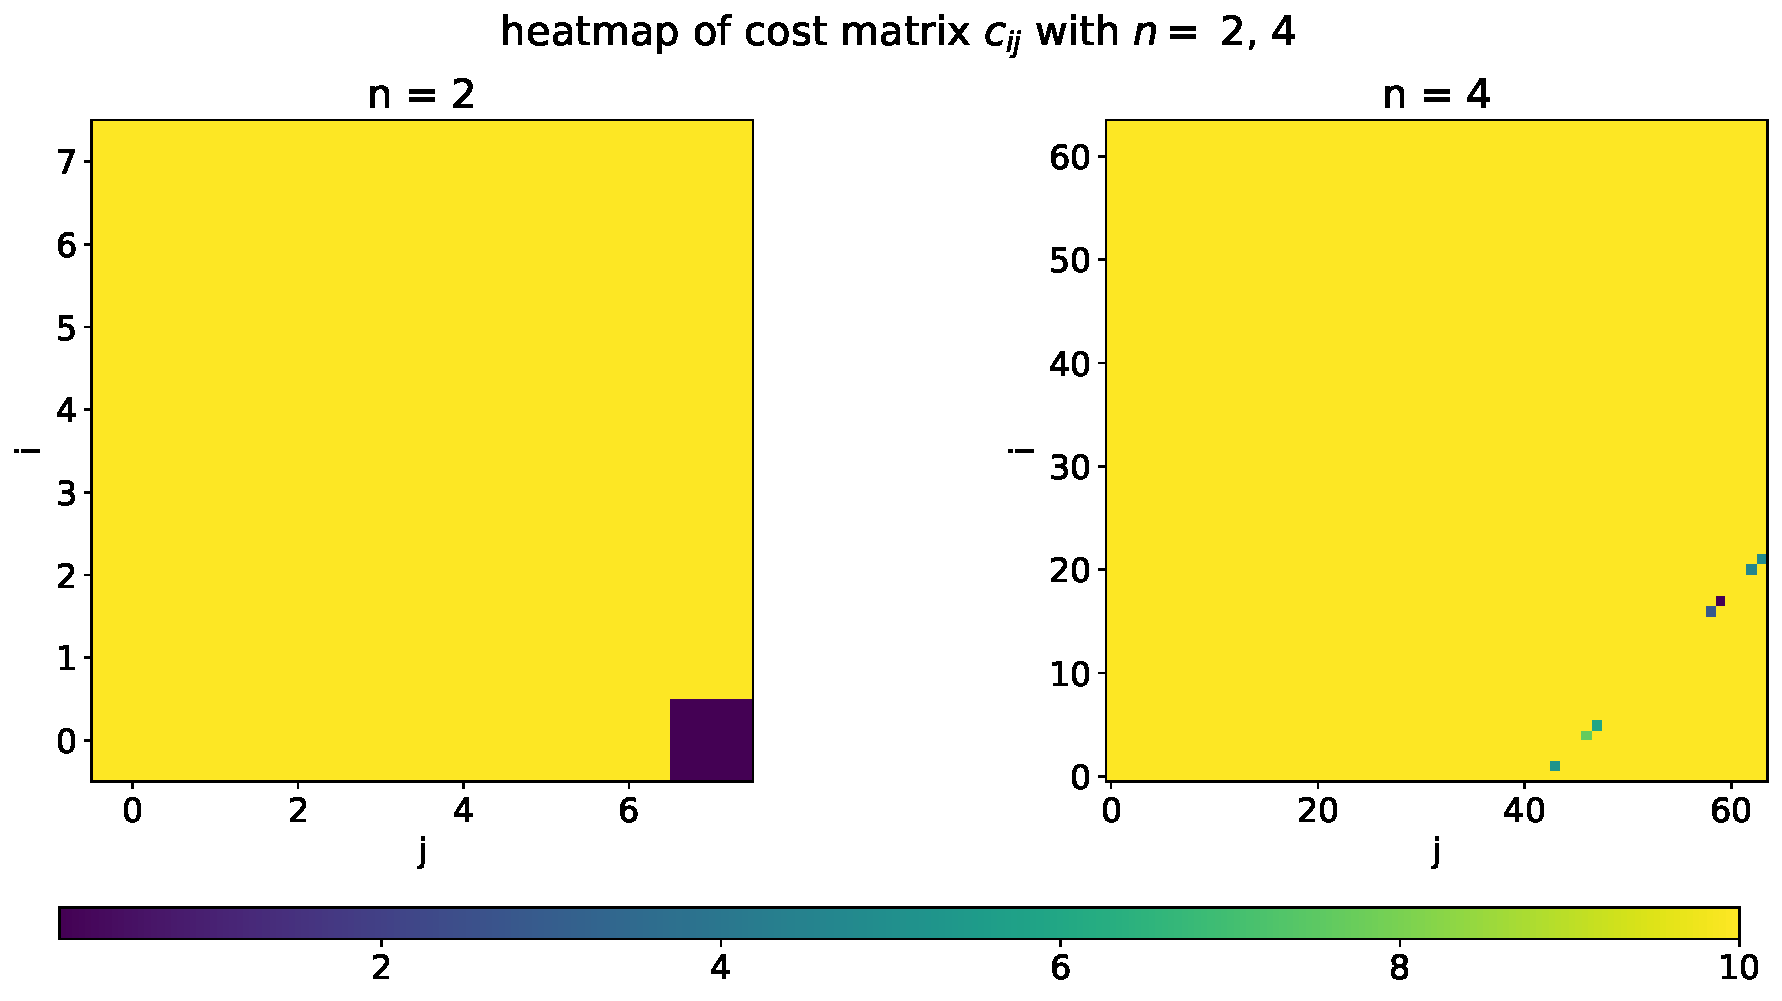
\includegraphics[width=\textwidth]{./images/uniform_v_ma_ncombined-n4-new.pdf}
	\caption{Heat map of the cost matrix for uniform linear motion from $[0, 50]^3$ to $[50, 100]^3$, for $n = 2$ (left) and $n = 4$ (right), as retrieved from Algorithm~\ref{alg:1}. The $n=2$ case is not scaled as described in Section~\ref{sec:refs}. }
	\label{fig:uniformlin}
\end{figure}
\begin{figure}[p]
	\centering 
	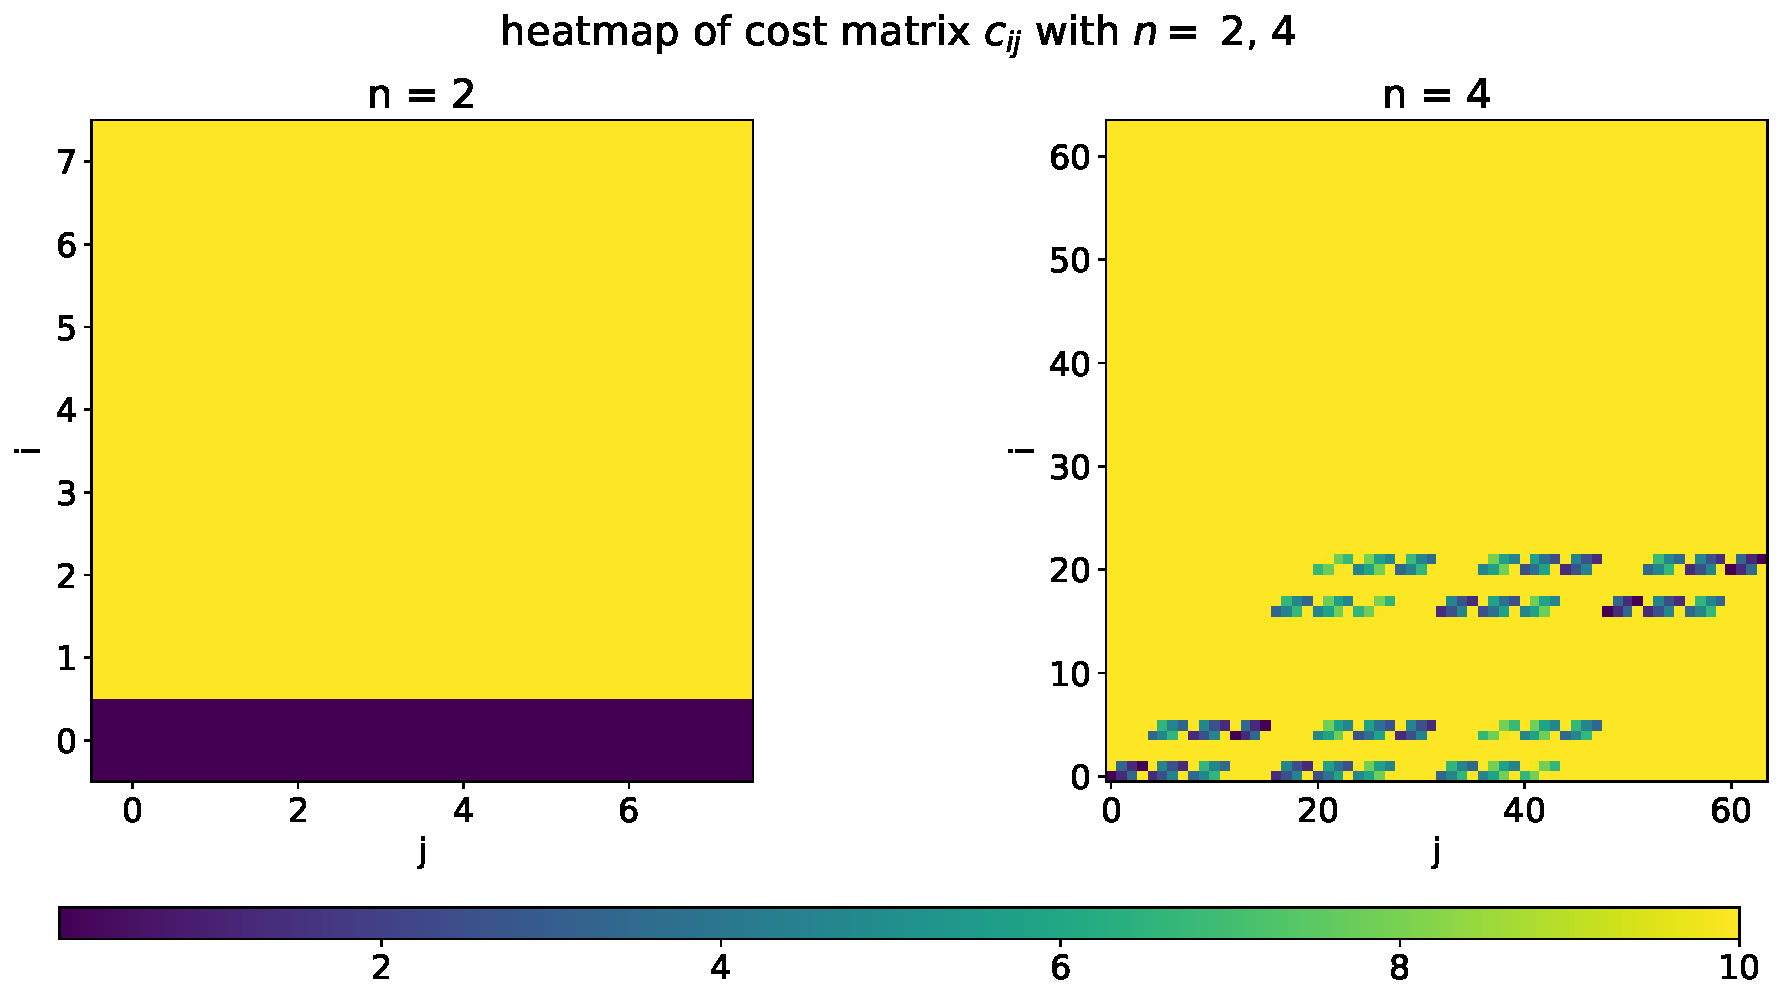
\includegraphics[width=\textwidth]{./images/nonuniform_v_ma_ncombined-n4-new.pdf}
	\caption{Heat map of the cost matrix for non-uniform linear motion from $[0, 50]^3$, for $n = 2$ (left) and $n=4$ (right), as retrieved from Algorithm~\ref{alg:1}. The $n=2$ case is not scaled as described in Section~\ref{sec:refs}. }
	\label{fig:nonuniformlin}
\end{figure}

Also for $n=4$ we can see a structure we would expect - there is some motion from $[0, 50]^3$, which is now divided into multiple boxes with low box number, to $[50, 100]^3$, which is divided into boxes with a higher box number. \par 
Note that, in general, the $n=2$ case is not the averaged $n=4$ case, due to the way the boxes are numbered, as box $0$ does not split into box $0, 1, 2$ and $3$. \par 
The same can be done for non-uniform motion. Let all the particles, again, go from $[0, 50]^3$, but add a non-linearity in the velocity. Now, the particles have $x$-, $y$- and $z$-velocities, which are not necessarily the same. Thus, particles can end up anywhere in $[0, 100]^3$. Again, it is expected that $\pihat_{ij}$ is high for a low $i$ (going from $[0, 50]^3$), and $\pihat_{ij}$ can be high for any $j$, since the particles can end up anywhere in $[0,100]^3$. Hence, we can expect that $c_{ij}$ is low for low $i$. Furthermore, more low-cost entries of $c$ are expected than in the uniform case. After all, all the particles did not move the same amount in $x$, so they might have gone to different boxes. \par 
As we can see in Figure~\ref{fig:nonuniformlin}, in the case $n=2$ we have indeed a very low cost moving away from box $0$ (where all particles started), and a high cost everywhere else, which is what was expected. Note that the $n=2$ case in Figure~\ref{fig:nonuniformlin} is, again, not scaled as described in Section~\ref{sec:refs}, as this scaling would result in a uniform heat map.\par 
For $n = 4$ in Figure~\ref{fig:nonuniformlin}, we can see more structure, but notably still only low cost for low values of $i$. The structure that can be seen is indeed a structure we would expect; there is some motion from the boxes in $[0, 50]^3$ to most other boxes. \par 
Thus, we can see that there are clear differences in the shape of the cost matrix with particle movements of constant and non-uniform velocity, which can be useful to determine structures in the cost matrix from the simulations. 

\subsection{Voids}
\label{sec:voids}
Forms of motion that are more common in the evolution of the Universe, are expansion and collapse \citep{planelles2014}. Let us consider (uniform and non-uniform) expansion, which tends to happen in voids. Again, a box size of $100$ (arbitrary units) is used. All data points start in a cube centered at $(50, 50, 50)$ with sides of $50$, and particles can move towards the whole box. \par 
We start by considering uniform expansion along three (spatial) dimensions. A scale factor can be calculated by using the initial and final radius, while scaling the points accordingly. Because we are considering particle to expand from a certain point, we can expect a symmetric cost matrix. Note that the axis of symmetry does not necessarily have to be the line $y = x$ (from $(0,0)$ to $(n^3, n^3)$), as the center of expansion is not necessarily in the center of a box, or in box $n^3/2$. Furthermore, for the $n=2$ case, no motion between boxes can be expected, as there is no side-to-side motion. This is indeed what we can see in Figure~\ref{fig:uniformexp}; we see a diagonal cost matrix. Note that the one square that has the same colour as the background, $c_{55}$, is due to the scaling as described in Section~\ref{sec:refs} and this is not inherent to the system. \par 
The case for $n=4$, which can also be seen in Figure~\ref{fig:uniformexp}, looks a bit more interesting. We can see that the cost seems to be almost symmetric in an almost diagonal line, which is what is to be expected for expansion. If we count the boxes, we can see that boxes $21, 22, 25, 26, 37, 38, 41$ and $42$ are indeed in the center of the (full) box. Movement from those boxes outwards, which is where we can see a lower cost in Figure~\ref{fig:uniformexp}, is indeed what we would expect.

\begin{figure}[p]
	\centering 
	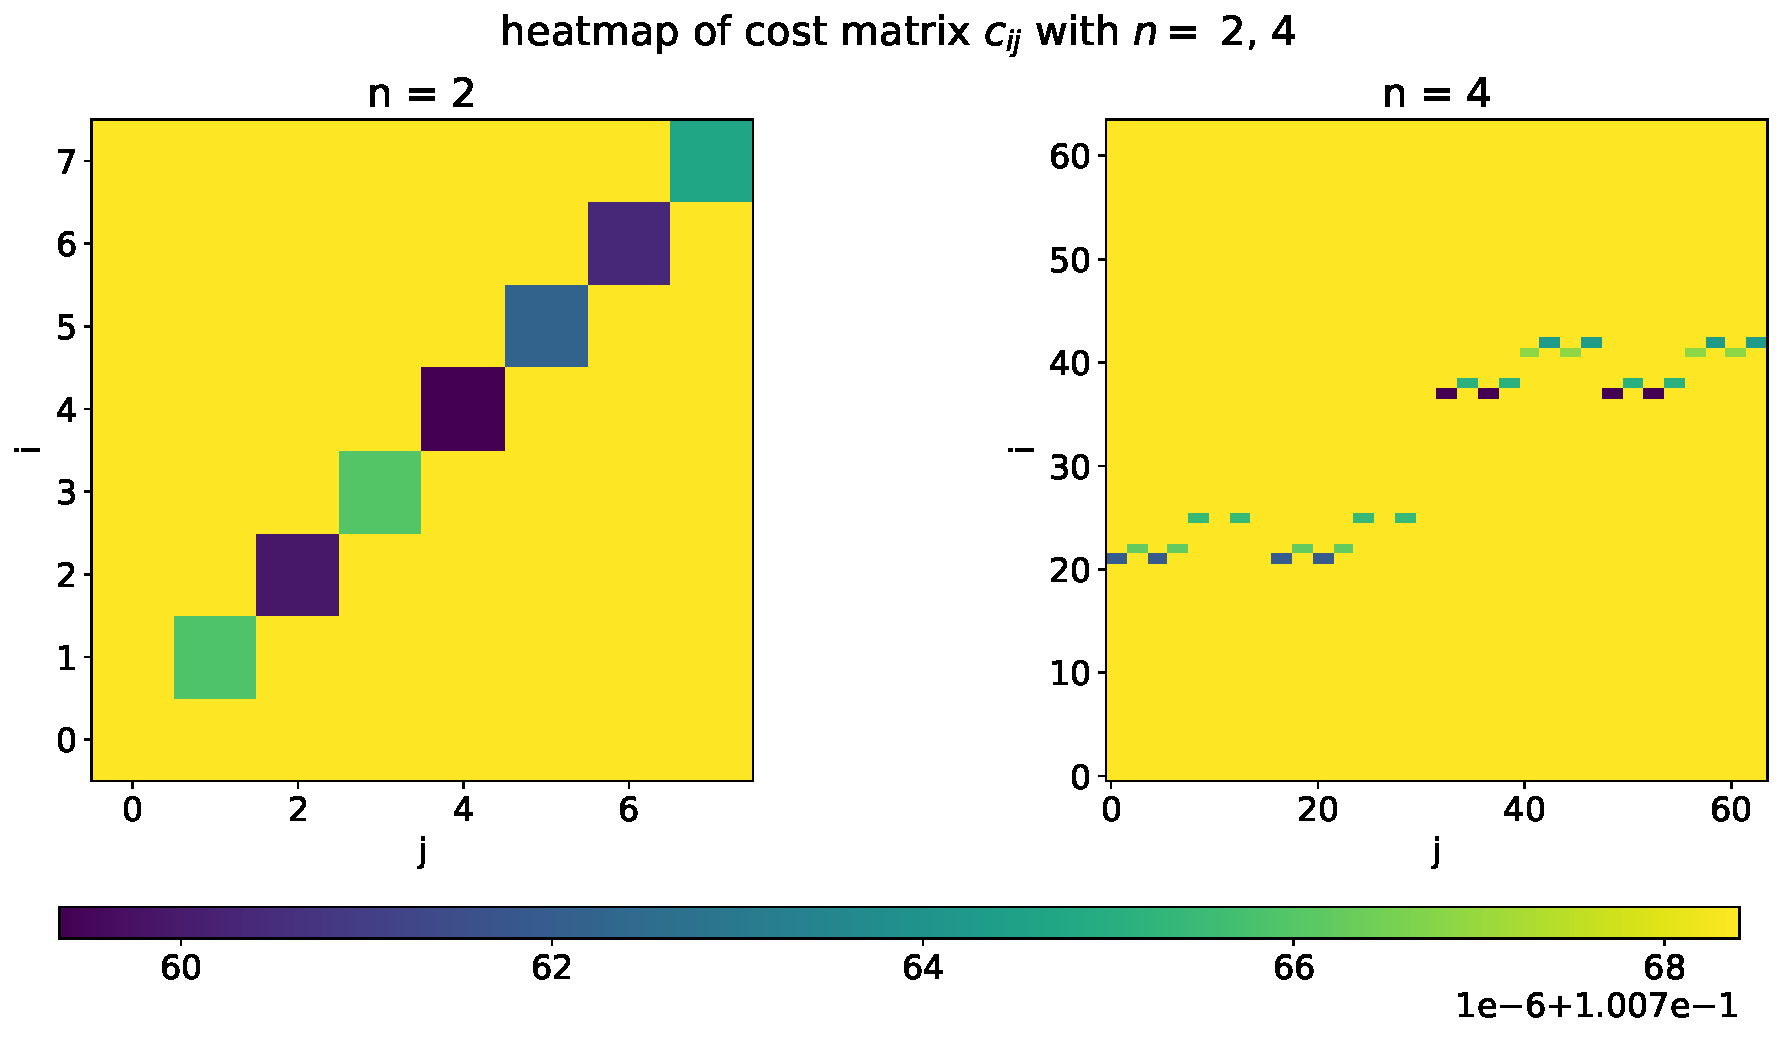
\includegraphics[width=\textwidth]{./images/uniform_expansion_ma_ncombined-n4-new.pdf}
	\caption{Heat map of the cost matrix for uniform expansion, for $n = 2$ (left) and $n = 4$ (right), as retrieved from Algorithm~\ref{alg:1}.}
	\label{fig:uniformexp}
\end{figure}
\begin{figure}[p]
	\centering 
	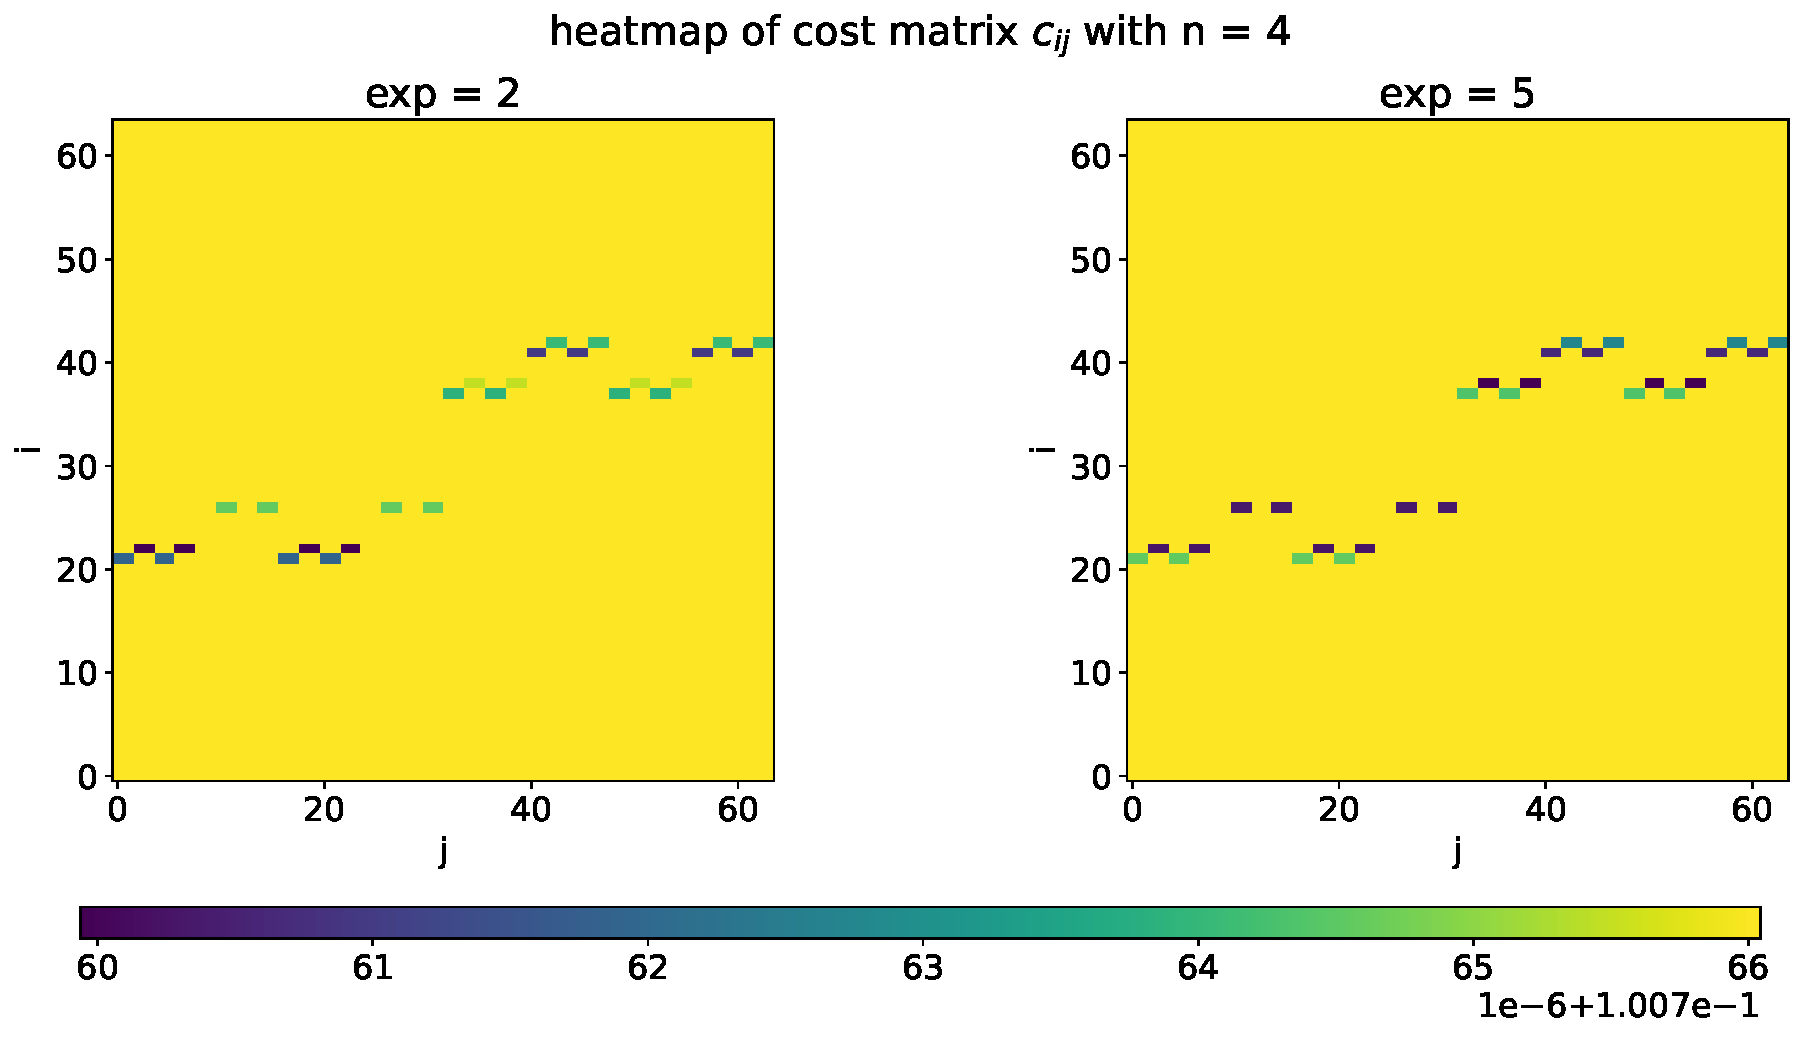
\includegraphics[width=\textwidth]{./images/nonuniform_expansion_ma_n4_c-combined-exp[2, 5]-new.pdf}
	\caption{Heat map of the cost matrix for non-uniform expansion, for both \lstinline|exp| $= 2$ (left) and \lstinline|exp| $=5$ (right), for $n = 4$, as retrieved from Algorithm~\ref{alg:1}. }
	\label{fig:nonuniformexpn4}
\end{figure}


Now, let us look at non-uniform expansion, again along three spatial dimensions. Here, one should choose how to simulate the non-uniformity. Physically, it makes the most sense to have accelerating expansion from a certain central point, in our case taken as the center point of our begin cube of points, which is the middle of the full box. The points will have an exponential velocity, depending on the distance from the center. This non-uniformity is implementing by using a parameter \lstinline|exp|.  When points are expanding from the initial sphere to a final, larger sphere, \lstinline|exp| controls the distribution of the radial displacement of each particle. Specifically, the initial distance of each particle from the center of expansion is calculated, and then normalized. This gives a set of normalized distances, \lstinline|normalized_distances|. These normalized distances then undergo a transformation where each element is raised to the power of \lstinline|exp|, \lstinline|scaled_normalized_distances = normalized_distances ** exp|. \par  
Note that if \lstinline|exp| $=1$, the expansion is uniform. For \lstinline|exp| $>1$, there is proportionally smaller displacement for particles closer to the center of expansion, than for particles that started far from the center of expansion, leading to a relatively dense distribution of particles near the center, and a relative thin distribution of particles further from the center of expansion. \par 
On the contrary, if $0 < $ \lstinline|exp| $<1$, points that are initially closer to the center of expansion will experience a proportionally larger outward displacement compared to particles that were further away initially. \par 
First, \lstinline|exp| is chosen to be $2$. For the $n=2$ case a fully diagonal cost matrix is again expected, as we still do not expect particles to move out of their boxes. Furthermore, the results for higher $n$ are very similar to those of the uniform expansion cases. The case $n=4$ can be seen in Figure~\ref{fig:nonuniformexpn4}. It is clear that the only difference to the $n=4$ case for uniform expansion is the scaling. Note that the "missing" squares in row $37$ or row $41$ in Figure~\ref{fig:nonuniformexpn4} are not inherent to the system, but rather a result of the scaling that was described at the beginning of this chapter. \par 
It is clear that the differences between uniform and non-uniform expansion are more subtle than that of uniform and non-uniform linear motion; the shapes of the cost matrix are the same. The differences are in the scaling, rather than the shape of the cost matrix. To see if there are differences visible for larger values of \lstinline|exp|, another exponent was tested, \lstinline|exp| $= 5$, as can also be seen in Figure~\ref{fig:nonuniformexpn4}, again for the $n=4$ case. We can indeed see that there is a different scaling for \lstinline|exp| $=5$. \par 
Note that the shapes of the cost matrices for \lstinline|exp| $= 5$ are still similar to the case of \lstinline|exp| $=2$, but the scaling indeed looks a bit different again. 
 
\subsection{Clusters}
\label{sec:clusters}
A third kind of motion to look at is collapse along three (spatial) dimensions, which tends to happen in clusters. For uniform and non-uniform collapse, we can do the same thing as we did for uniform and non-uniform expansion, but with a scale factor $< 1$. Here, we start with points in the whole box, of length $100$. The particles will end in a cube with sides of length $50$, centered at $(50, 50, 50)$. Due to the way the data points are generated, as with the expansion cases, a fully diagonal cost matrix is expected for the $n=2$ cases, so we will not go into this case any further. \par 

\begin{figure}[p]
	\centering 
	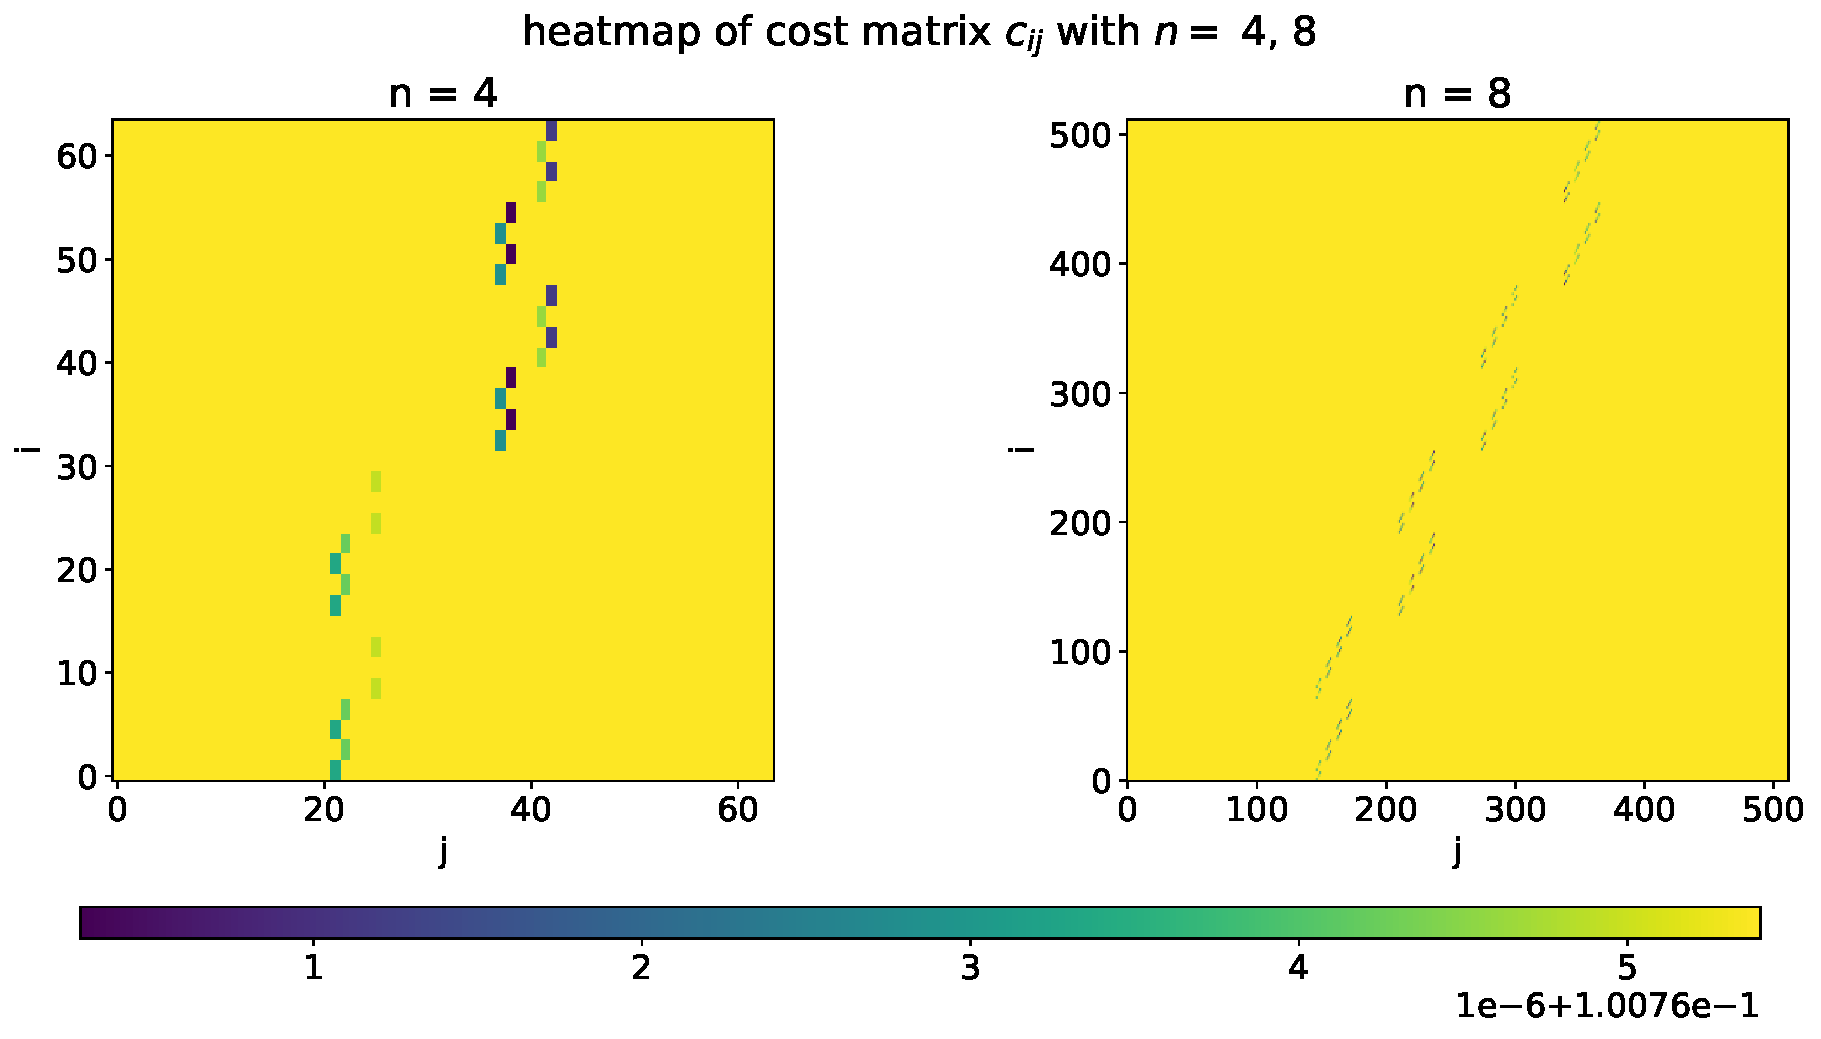
\includegraphics[width=\textwidth]{./images/uniform_collapse_ma_ncombined-n8-new.pdf}
	\caption{Heat map of the cost matrix for uniform collapse, for $n = 4$ (left) and $n = 8$ (right), as retrieved from Algorithm~\ref{alg:1}.}
	\label{fig:unifcoll}
\end{figure}

\begin{figure}[p]
	\centering 
	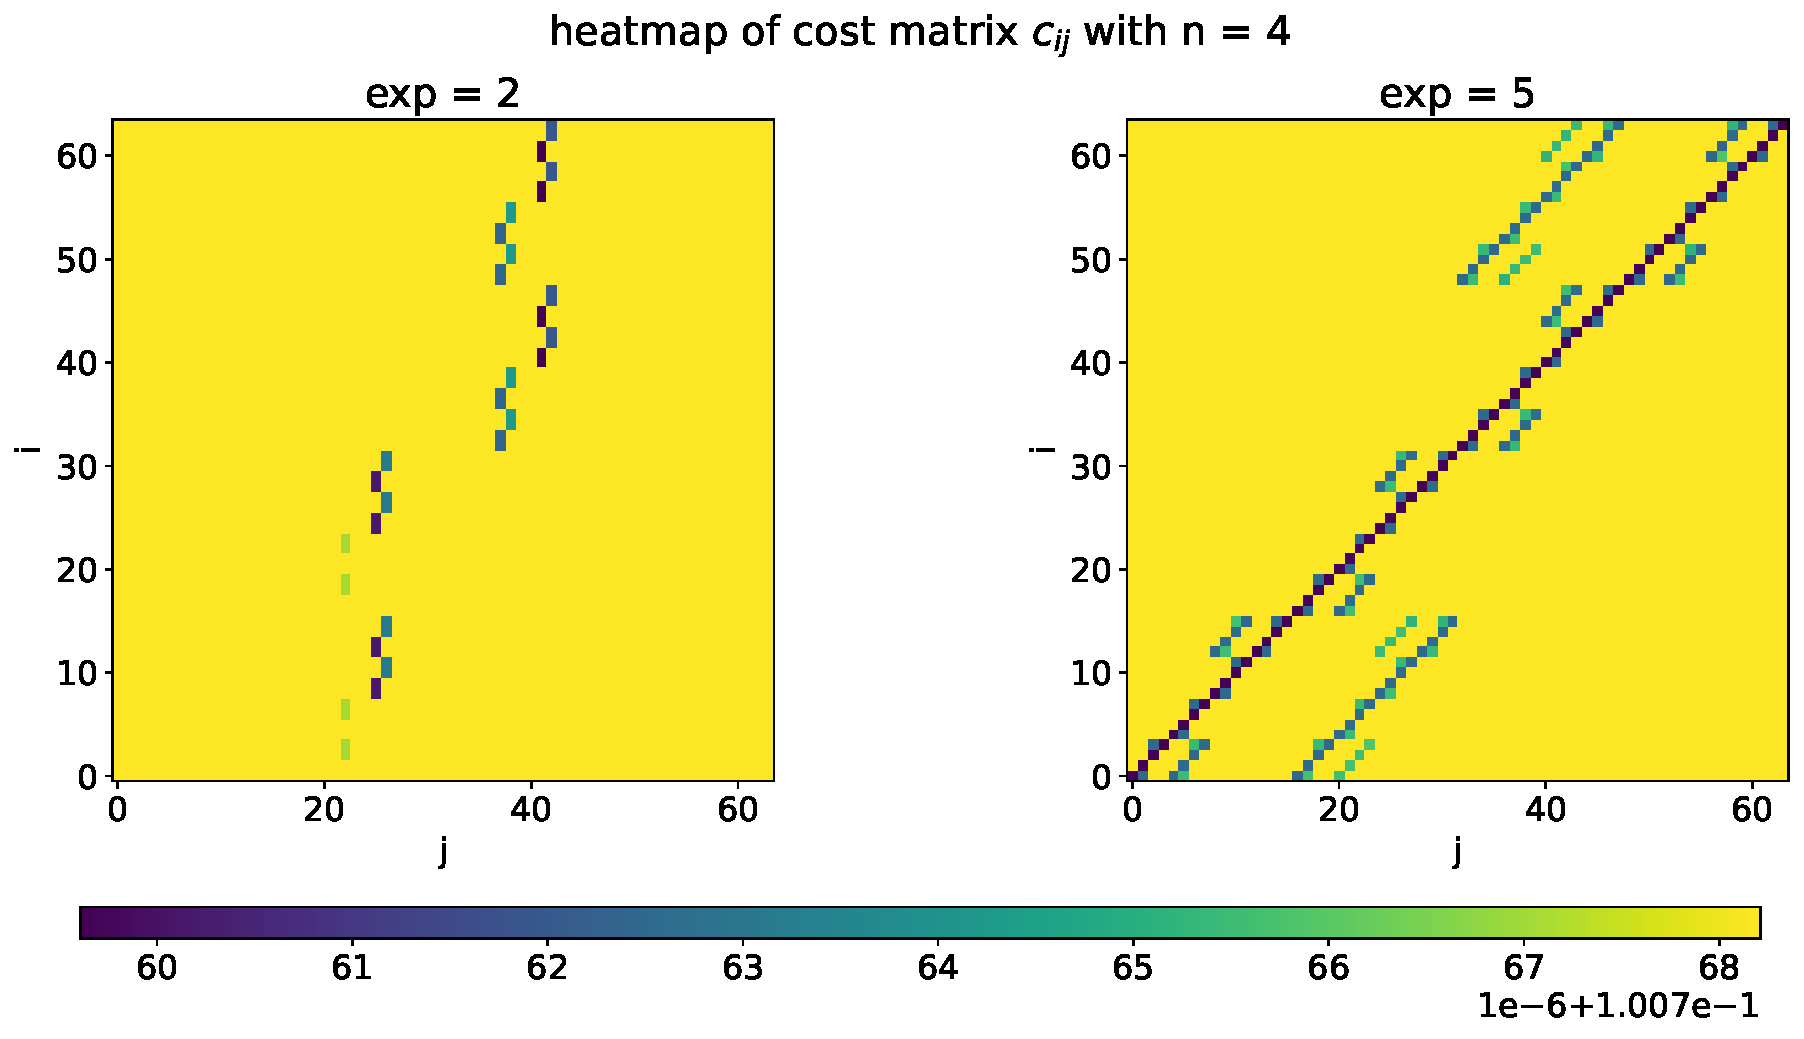
\includegraphics[width=\textwidth]{./images/nonuniform_collapse_ma_n4_c-combined-exp[2, 5]-new.pdf}
	\caption{Heat map of the cost matrix for non-uniform collapse, for both \lstinline|exp| $=2$ (left) and \lstinline|exp| $=5$ (right), for $n = 4$, as retrieved from Algorithm~\ref{alg:1}. }
	\label{fig:nonuniformcolln4}
\end{figure}

For uniform collapse, we can see for the case $n=4$, in Figure~\ref{fig:unifcoll}, what looks like a $90$ degree rotation of the cost matrix with respect to the uniform expansion case, in Figure~\ref{fig:uniformexp}. This is to be expected, as if we time-invert the expansion, we get a collapse process. Thus, you would expect $\pihat^c_{ij} = \pihat^e_{ji}$, with $\pihat^c$ the transportation matrix of collapse, and $\pihat^e$ the transportation matrix of expansion. Hence, we would also expect $c^c_{ij} \approx c^e_{ji}$, again with $c^c$ the cost matrix of collapse, and $c^e$ the cost matrix of expansion. This rotation of the expansion case is indeed what we can see in Figure~\ref{fig:unifcoll}. \par 
For the $n=8$ case, also in Figure~\ref{fig:unifcoll}, we can see that the structure is quite similar to the $n=4$ case. Again, the values of where the cost is lower can be explained by counting out the boxes and seeing where we would physically expect particles to go. \par 
If we look at non-uniform collapse, we expect for lower \lstinline|exp| structures that are quite similar to those of non-uniform expansion. In Figure~\ref{fig:nonuniformcolln4} we can see the $n=4$ case for \lstinline|exp| $=2$, which looks like a $90$ degree rotation of Figure~\ref{fig:nonuniformexpn4}, the non-uniform expansion case for $n=4$ and \lstinline|exp| $=2$.  \par 
However, when we increase \lstinline|exp|, we can see different structures emerging. In Figure~\ref{fig:nonuniformcolln4}, for $n=4$ and \lstinline|exp| $=5$, a wide, more diagonal structure can be seen, clearly distinguishable from the earlier \lstinline|exp| $=2$ case. Note that in this case, the cost matrix is clearly not a rotation of the expansion cost matrix in Figure~\ref{fig:nonuniformexpn4}. This discrepancy is probably due to the fact that the process of non-uniform expansion and collapse are not time-reversible in the same way as uniform expansion and collapse. The main reason for this discrepancy could be the asymmetry that is introduced by the non-uniformity. 


\subsection{Walls}
Another common type of motion in cosmology is a combination of expansion and collapse. One example of combination of expansion and collapse is walls (or sheets). Walls are flattened, sheet-like structures that enclose the voids, and are associated with collapse along one dimension (perpendicular to the wall), and expansion along the other two dimensions (within the plane of the wall) \citep{bos2016}. Simulations were made of these walls, again with a box size of $100$ (arbitrary units), and points started in a cube centered at $(50, 50, 50)$ with sides of length $50$. Different values for \lstinline|exp| for the expansion and collapse can be taken. We chose to consider the case where \lstinline|exp| $:=$ \lstinline|exp|$_\text{collapse}$ = \lstinline|exp|$_\text{expansion}$. The cases \lstinline|exp| $=2$ and \lstinline|exp| $=5$ were studied, as can be seen in Figure~\ref{fig:wallse1} for $n=4$. \par 
In Figure~\ref{fig:wallse1}, it can be seen that the values of the cost matrix that are not $M_c$ are around the same places as in the expansion and collapse cases. However, a different structure than in the pure collapse and expansion cases can be seen, with less values not equal to $M_c$. Because the initial condition for $n=4$ was a cube that was only in eight boxes to begin, box 21, 22, 25, 26, 37, 38, 41 and 42, we would only expect a non-$M_c$ cost in these boxes on the $i$-axis. This is indeed what we can see in both figures in Figure~\ref{fig:wallse1}. Then, with collapse along one dimensions, one would not expect much movement outward in the direction of this dimension, adding diagonal values to the cost matrix. However, from expansion along the other two dimensions, one would expect the particles to move towards other boxes, corresponding to the off-diagonal values. 

\begin{figure}[p]
	\centering 
	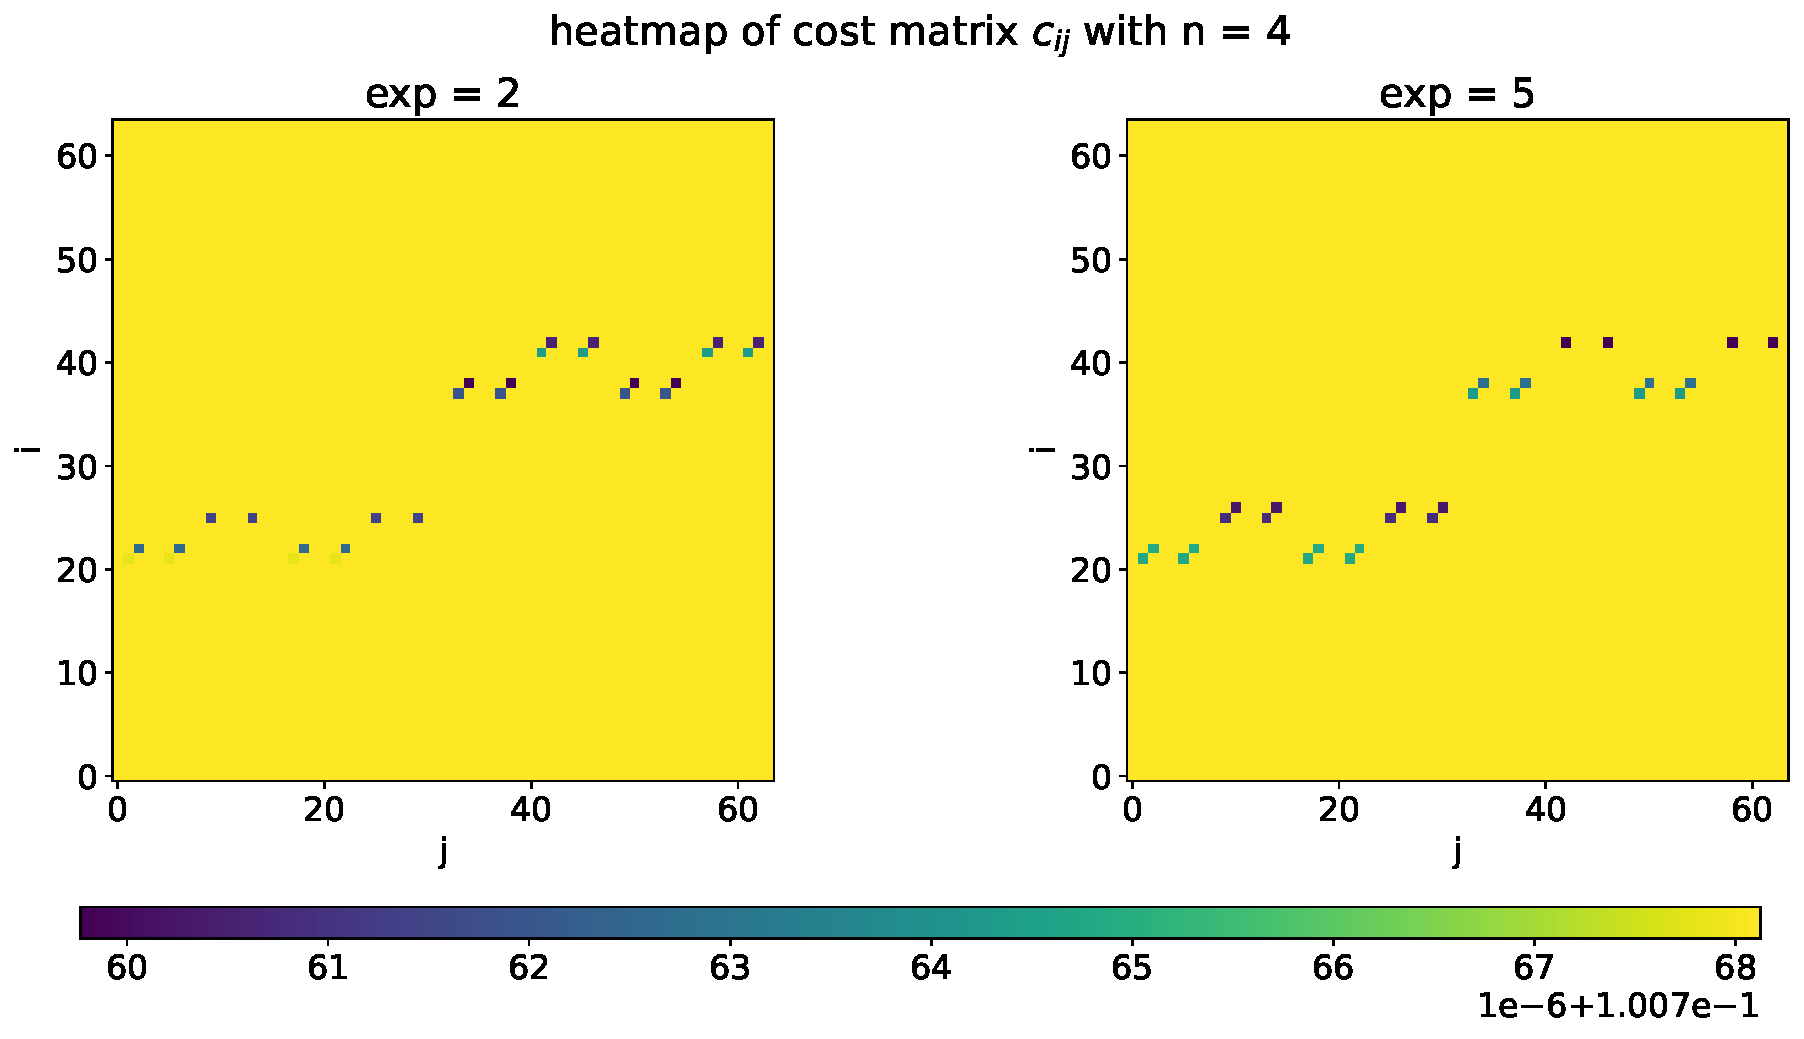
\includegraphics[width=\textwidth]{./images/walls_ma_n4_c-combined-exp[2, 5]-new.pdf}
	\caption{Heat map of the cost matrix for walls, for both \lstinline|exp| $=2$ (left) and \lstinline|exp| $=5$ (right), for $n = 4$, as retrieved from Algorithm~\ref{alg:1}. }
	\label{fig:wallse1}
\end{figure}

\begin{figure}[p]
	\centering 
	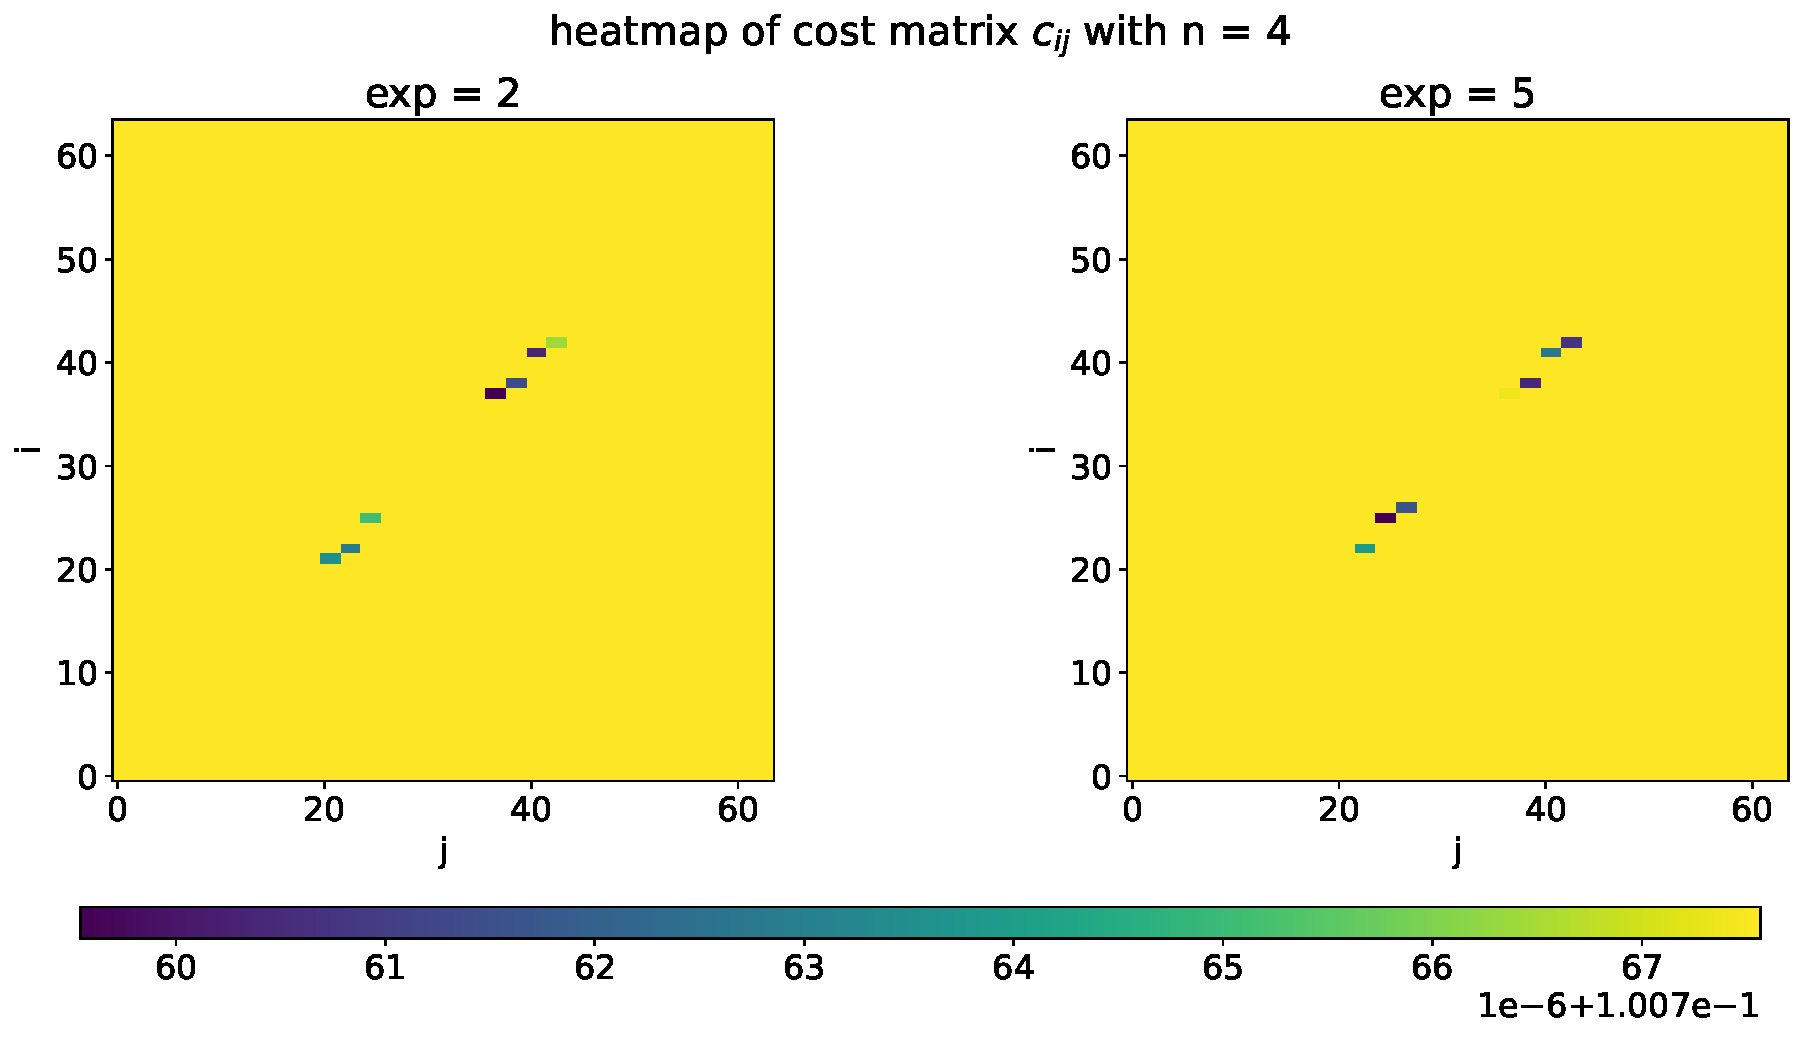
\includegraphics[width=\textwidth]{./images/filament_ma_n4_c-combined-exp[2, 5]-new.pdf}
	\caption{Heat map of the cost matrix for filaments, for both \lstinline|exp| $=2$ (left) and \lstinline|exp| $=5$ (right), for $n = 4$, as retrieved from Algorithm~\ref{alg:1}.  }
	\label{fig:filaments}
\end{figure}


\subsection{Filaments}
As a last reference case, we will look at another mixed expansion-collapse case, filaments. Filaments are associated with collapse along two dimensions (perpendicular to the filament's axis), and expansion/flow of matter along the other dimension \citep{bos2016}. We will model the latter as expansion. These simulations were made again with a box size of $100$ (arbitrary units), and points started in a cube centered at $(50, 50, 50)$ with sides of length $50$. Different values of \lstinline|exp| for the expansion and collapse can be taken. We chose, as for the walls, to consider the case where \lstinline|exp| $:=$ \lstinline|exp|$_\text{collapse}$ = \lstinline|exp|$_\text{expansion}$. Again, the cases \lstinline|exp| $=2$ and \lstinline|exp| $=5$ were studied, as can be seen in Figure~\ref{fig:filaments} for $n=4$. \par  
We can see that for $n=4$, there are very few cases where the cost matrix is not equal to $M_c$, all of which are approximately on the diagonal. This is probably due to the case that we started with a cube that was only in eight boxes to begin with, box 21, 22, 25, 26, 37, 38, 41 and 42. Therefore, on the $i$-axis, we would only expect a non-$M_c$ cost here, which is indeed what we can see in both figures in Figure~\ref{fig:filaments}. Then, with collapse along two dimensions, one would not expect much movement outward. Hence, the particles are expected to stay in, or close to, their own boxes in the $n=4$ case. 

\section{FLAMINGO Cost Matrix}
Using Algorithm~\ref{alg:1}, the cost matrix of the FLAMINGO data, as described in Chapter~\ref{ch:data}, can be found. With the reference cases described in Section~\ref{sec:refs}, we hope to interpret this cost matrix. First, we will comment on the expected cost matrix, whereafter the cost matrix as recovered from Algorithm~\ref{alg:1} will be discussed. 

\subsection{Expected Cost Matrix}
As described before in Chapter~\ref{ch:data}, the FLAMINGO simulations are hydrodynamical cosmological simulations, with the aim to understand the large-scale structure formation of the universe. Hence, knowledge about the expected large-scale structures can be used to comment on the expected cost matrix.

\subsubsection{Structure Formation in the Cosmic Web}
In large-scale structure formation, one would expect filaments, voids, sheets/walls and clusters to form, arising from the gravitational collapse of a relatively uniform initial density distribution in the early Universe. These different structures have different motions associated with them \citep{bos2016}. Voids are vast, under-dense regions, largely without many galaxies or matter. They are characterized by expansion along all three dimensions, effectively pulling matter out of the void towards the surrounding denser structures. Walls (or sheets) are flattened, sheet-like structures that enclose the voids. The walls are denser than voids, but less dense than filaments or clusters. As mentioned before, walls are associated with collapse along one dimension (perpendicular to the wall), and expansion along the other two dimensions (within the plane of the wall). Hence, matter is flowing inwards towards the central plane of the wall, while stretching out within that plane as it gets pulled towards the denser filaments and clusters. Filaments are elongated, thread-like structures. Filaments primarily have collapse along two dimensions (perpendicular to the filament's axis), and expansion/flow of matter along the other dimension. Lastly, clusters are the densest and most massive regions in the Cosmic Web. They are gravitationally bound, and therefore have (gravitational) collapse in all three dimensions. As we expect all of these cases to occur in our data, we expect the cost matrix to be some combination of these cases, and therefore a combination of our reference cases.

\subsubsection{Geodesics}
On a single-particle level, the particles are expected to take the locally shortest path between their initial and final position. Therefore, the particles are expected to move along the geodesics as recovered from General Relativity. Hence, the cost matrix is expected to comply with the laws of General Relativity and the $\Lambda$CDM paradigm, as the FLAMINGO simulations are based on these laws \citep{schaye2023}. Thus, if one were to have a very high resolution, in our case computational resolution, the problem of the search for a cost matrix could be stated in a way to be a test of General Relativity. If one were to observe particle motion in larger-scale structures in the real universe and find a cost matrix from those movements, one could check the observed cost matrix against the theoretical cost matrices from the simulations. With this comparison, one could possibly infer the cosmological parameters. However, this goes beyond the scope of this thesis, so we will not discuss it any further. 

\subsection{Recovered Cost Matrix}
With the knowledge of what we expect for the cost matrix in mind, Algorithm~\ref{alg:1} can be implemented the same way as for the reference cases in Section~\ref{sec:refs} to find the cost matrix of the FLAMINGO data. The results can be seen in Figure~\ref{fig:data}, scaled in the same was as described in Section~\ref{sec:refs}. For the $n=4$ case, in Figure~\ref{fig:datan4}, we can already see that the structure of the cost matrix is more complicated than the previous reference cases, which is what is to be expected. It is expected that there is quite a lot of local collapse and expansion going on, in contrast to the only one scale of expansion and collapse in the reference cases. However, this makes it difficult to interpret the cost matrix on first sight. \par 
For $n=8$, in Figure~\ref{fig:datan8}, the cost matrix looks quite similar to the $n=4$ case, still with the diagonal stripes. However, it is also clear that this is quite far from any reference case in Section~\ref{sec:refs}. \par 

\begin{figure}[p]
	\centering
	\subfloat[Cost matrix with $n=4$.]{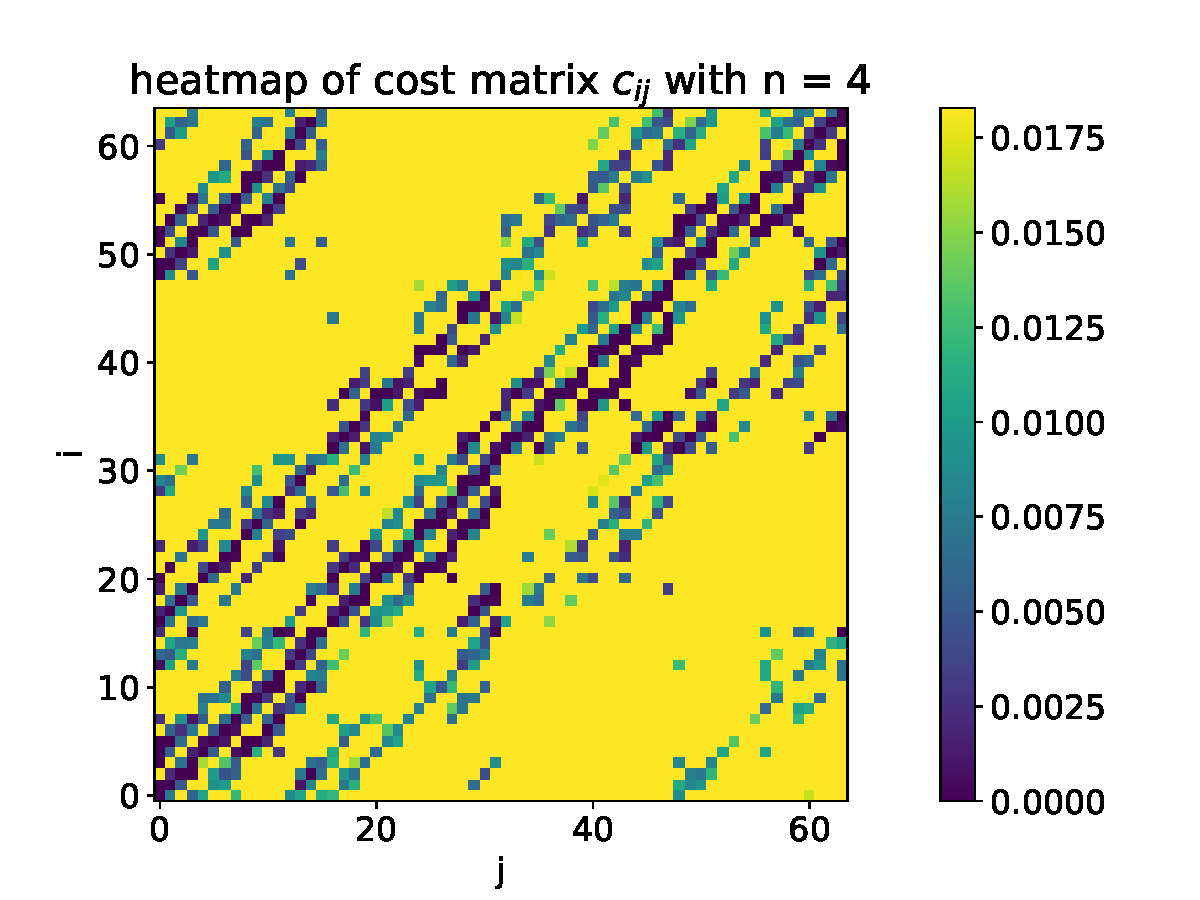
\includegraphics[width=0.8\textwidth]{./images/c-n4-new-zeros.pdf}\label{fig:datan4}}
	\\
	\subfloat[Cost matrix with $n=8$.]{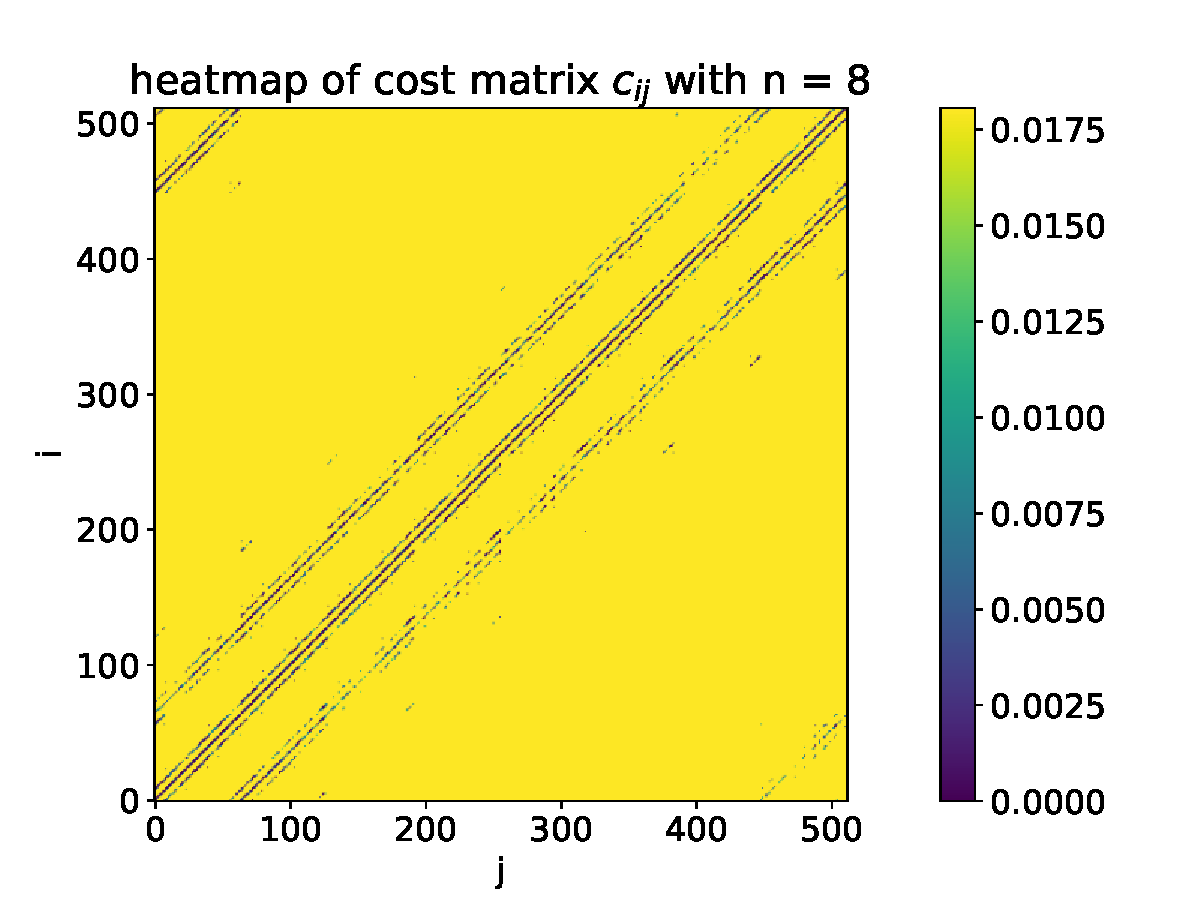
\includegraphics[width=0.8\textwidth]{./images/c-n8-new-zeros.pdf}\label{fig:datan8}}
	\caption{Heat map of the cost matrix for the FLAMINGO data, for $n = 4$ and $n = 8$, as retrieved from Algorithm~\ref{alg:1}.}
	\label{fig:data}
\end{figure}

As touched on before, it is expected that there is a lot of different kinds of motion going on in the simulation, and it is difficult to visually distinguish the different motions from these cost matrices. Note, however, that both cost matrices in Figure~\ref{fig:data} look quite symmetric, which implies isotropy and is what is to be expected from the cosmological principle.

\subsection{Markov Chain Monte Carlo Simulation} 
One way to interpret these results is through the assumption that the FLAMINGO results are a linear combination of multiple different reference cases. \par 
To test this assumption, simulations of more reference cases were done, without the simulation necessarily filling the whole box. For better computational efficiency, $500$ thousand particles were simulated instead of $1$ million as in Section~\ref{sec:refs}. Particles were simulated to expand from a cube of length $50$ (arbitrary units) to a cube of length $100$, or to collapse from a cube of length $100$ to a cube of length $50$. The box size was chosen to be $400$. Multiple centers for the expansion were chosen: $(x, y, z)$ with $x, y, z \in \{100, 200, 300\}$, as well as multiple values of \lstinline|exp|, \lstinline|exp| $\in \{0.4, 1, 2, 5\}$. With this, $27$ reference cases for each type of motion were made, all with $4$ \lstinline|exp| values, and both for expansion and collapse. This resulted in 216 reference cases. However, it is expected that this is not enough, as there is only expansion and collapse possible from a limited number of points in the box. \par 
As a proof of concept to test the hypothesis that the FLAMINGO cost matrix is a linear combination of the reference cases, a Markov Chains Monte Carlo (MCMC) simulation was used. For MCMC, one needs to consider Bayes' formula \citep{grimmett2014}: 
\begin{equation}
	\P(A|B) \propto \P(B|A) \P(A),
\end{equation}
with $\P(A|B)$ the posterior probability, $\P(B|A)$ the likelihood and $\P(A)$ the prior. Here, $A$ can be seen as the model, and $B$ as the data. A Gaussian prior was used, 
\begin{equation}
	\P(A) = \prod_i e^{-(\theta_i - \hat{\theta}_i)^2/2\sigma_i^2},
\end{equation}
with $\theta$ a vector of model parameters, $\hat{\theta}_i$ the initial guess for parameter $\theta_i$, and $\sigma_i$ the width of the prior. Note that $\sigma_i$ should be large enough to allow the model to move away from the initial guess $\hat{\theta}$, but not so large that it jumps into regions deemed unrealistic and therefore having a higher computational cost then necessary. To ensure numerical stability, a simple bound that returns negative infinity if any of the input elements were bigger than some limit was added to this Gaussian prior, where we used a limit value of $1000$. A similar bound on the parameter values was implemented to ensure all parameters are non-negative. For the likelihood, a Gaussian was also used. For all $\sigma_i$, a value of $0.5$ was used. \par 
The Python library \lstinline|emcee| is used for the MCMC simulation \citep{emcee}. The simulation was run by 1000 walkers and 5000 steps for each walker. We will get some randomly generated, uniformly distributed starting positions, and set up and run a sampler afterwards. Then, we will need to look at the best values for the fit, and marginalize the data, using 
\begin{equation}
	P(a|B) = \int P (a,b|B) \d b,
\end{equation}
where $a$ and $b$ are parameters of the fit. The median of the distribution will be calculated as the best value, and the $16$th and $84$th percentiles as the uncertainty range. \par 
For the MCMC, we used cost matrices with $n=8$, so $8^3$ boxes. Cost matrices with $n=8$ for the reference cases are discussed in Appendix~\ref{sec:apprefs}. We can see the evolution of the walkers for the first few parameters in Figure~\ref{fig:mcmcwalkers}. \par 
\begin{figure}[p]
	\centering
	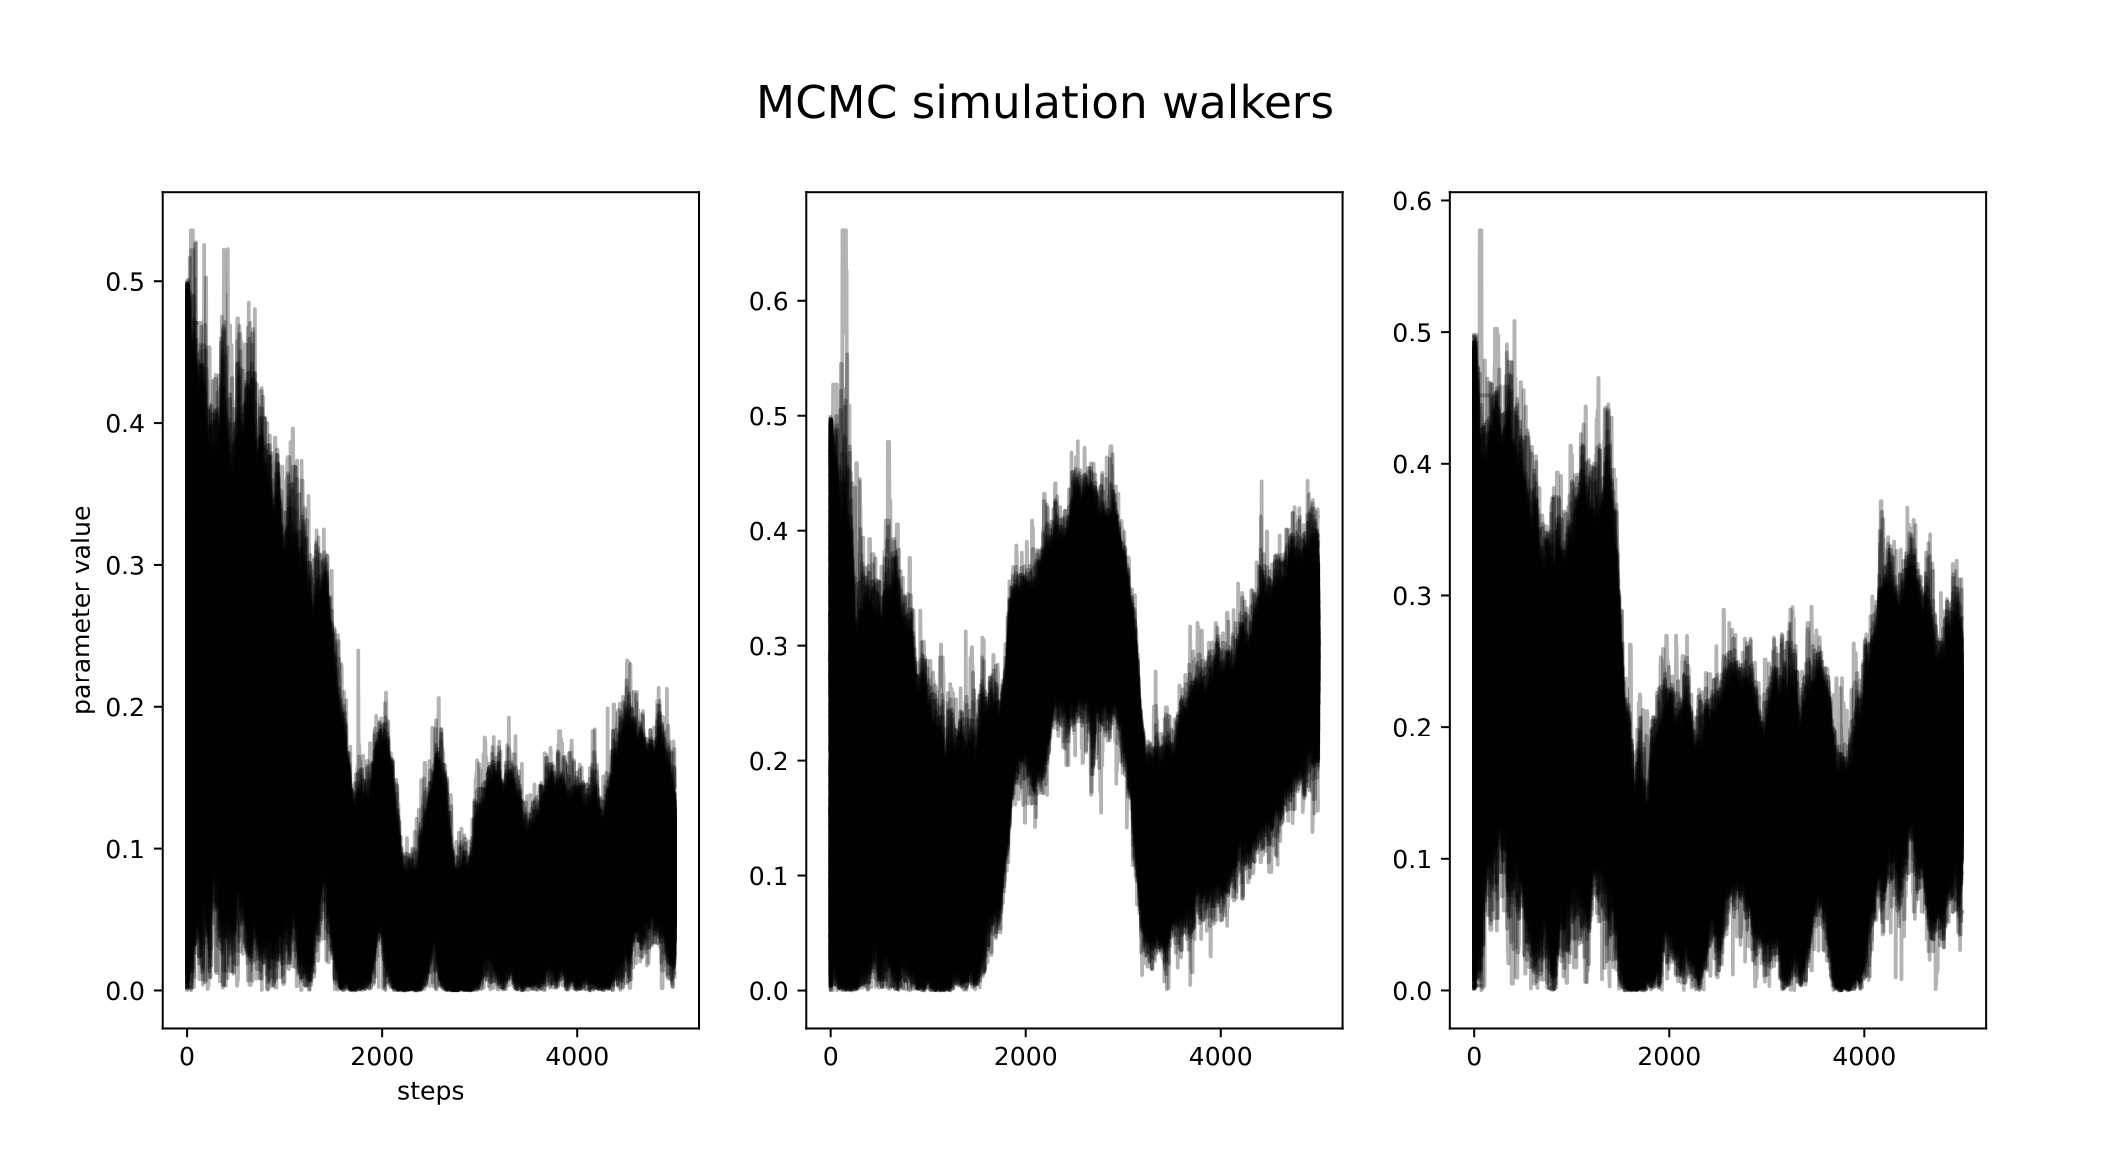
\includegraphics[width=\textwidth]{images/sampler.png}
	\caption{MCMC walkers for the first few parameters; expansion from $(100, 100, 100)$ (left), expansion from $(100, 100, 200)$ (middle) and expansion from $(100, 100, 300)$ (right).}
	\label{fig:mcmcwalkers}
\end{figure}

We can see that the chains are not converging well. This aligns with our expectation that the 216 described reference cases are not enough. The expectation is that more reference cases will solve this issue, but we cannot rule out the possibility that the FLAMINGO data is not a linear combination of the described reference cases or our initial guesses of parameters were too far off. \par 

\begin{figure}[p]
	\centering
	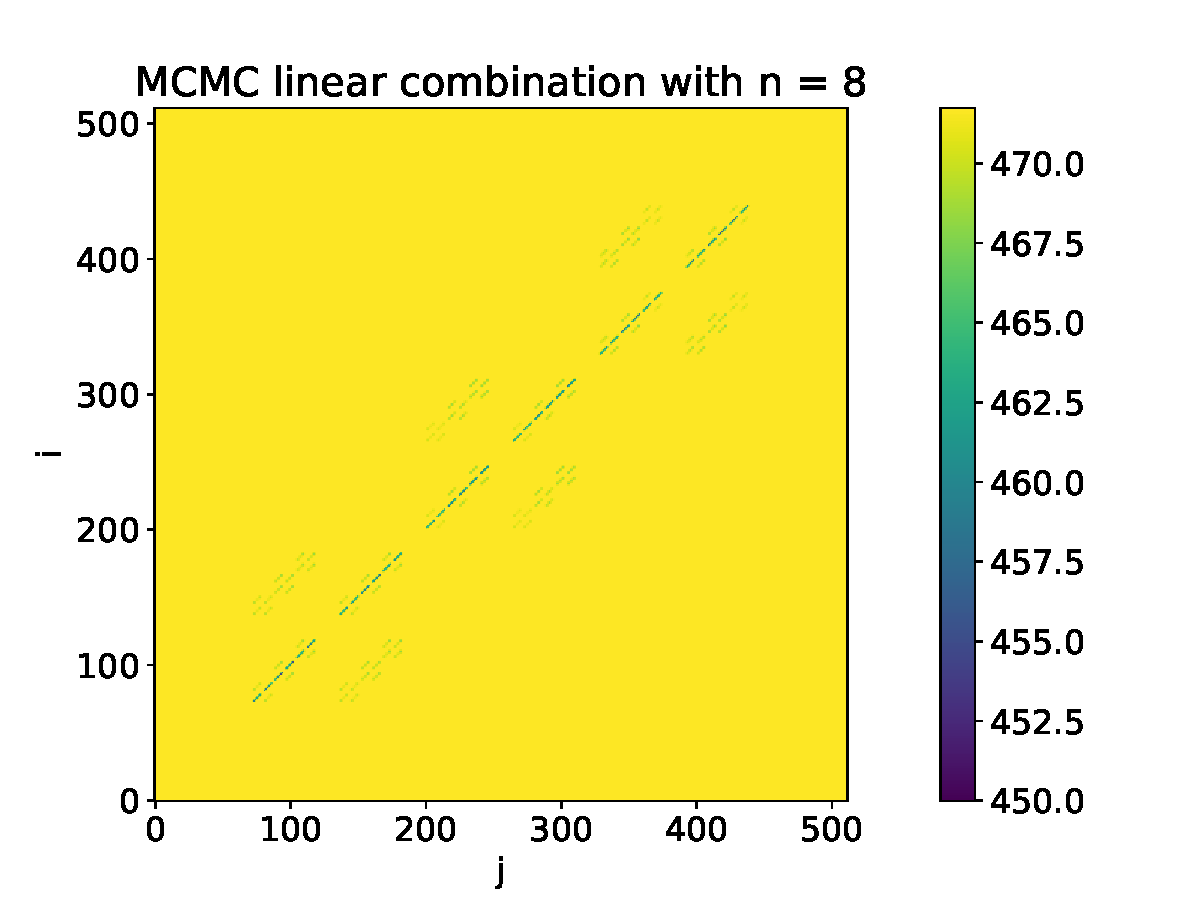
\includegraphics[width=0.8\textwidth]{images/mcmc_cost}
	\caption{Cost matrix from the linear combination of the MCMC, with $n=8$.}
	\label{fig:mcmccost}
\end{figure}

The cost matrix from these MCMC results can be seen in Figure~\ref{fig:mcmccost}. As described before, the median value is used as best-fit parameter. It can be seen that the values of this cost matrix are indeed far off from the FLAMINGO data, in Figure~\ref{fig:data}. \par 
To better show how far off this cost matrix is, the differences between the FLAMINGO cost matrix and the cost matrix from the linear combination of the MCMC can be seen in Figure~\ref{fig:mcmcdiffs}. It is clear that the MCMC fit is not a good fit and does not describe the data well. 


\begin{figure}[!ht]
	\centering
	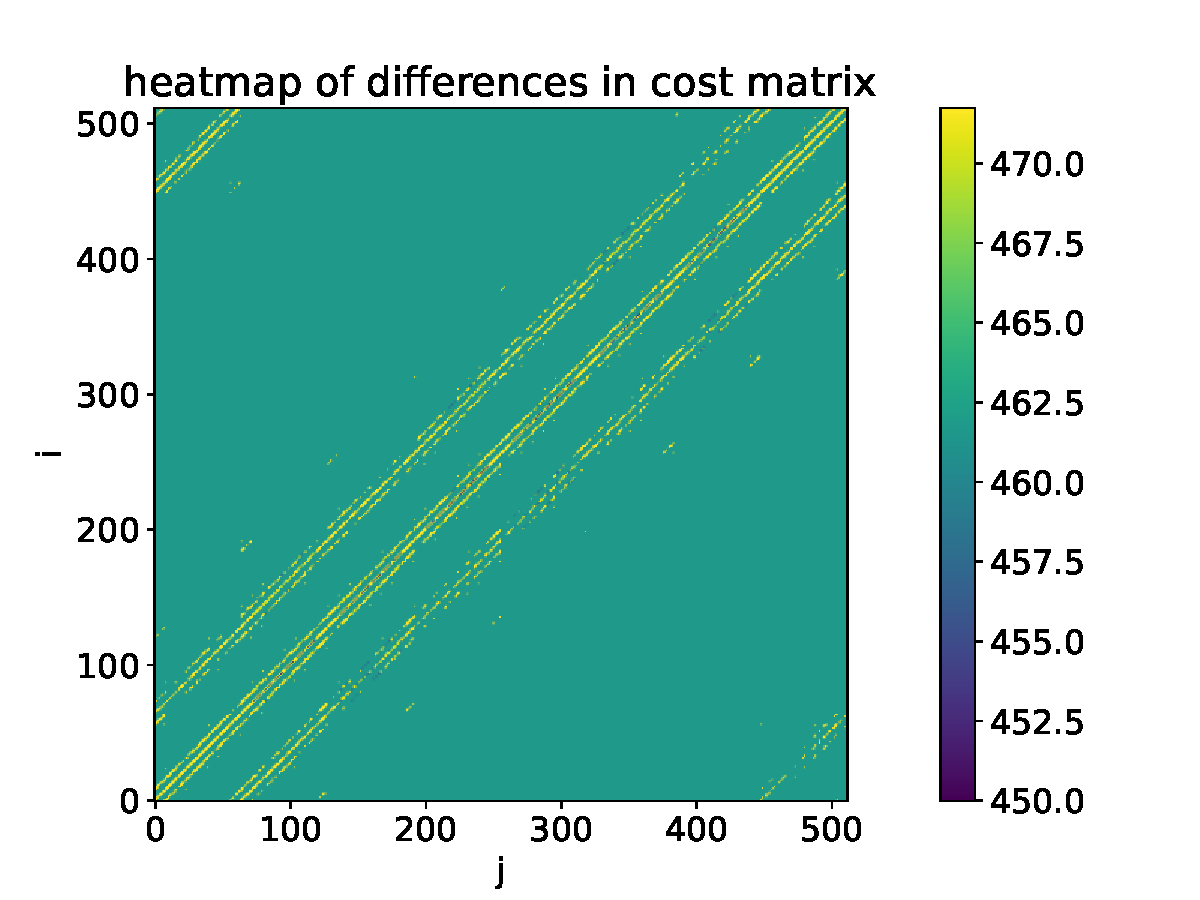
\includegraphics[width=0.8\textwidth]{./images/costmatrix-mcmc-diff.pdf}
	\caption{Differences between the FLAMINGO cost matrix and the cost matrix from the linear combination of the MCMC, for $n=8$.}
	\label{fig:mcmcdiffs}
\end{figure}



















\chapter{Outlook}
The research presented in this thesis aimed to characterize the evolution of the Universe through the lens of inverse Optimal Transport (OT). The FLAMINGO simulations were chosen as suitable simulations to work with, and the data was divided into smaller boxes for computational efficiency. The aim was to find a cost matrix that describes the motion of the particles within the simulations. In Chapter~\ref{ch:entropyregiOT}, an algorithm was developed for applying inverse OT, and comments were made on the equivalence of different solutions, as in general inverse OT problems can be ill-posed. This algorithm was inspired by \citet{ma2021}, with their proofs being discretized as can be seen in Appendix \ref{ch:proofs}. The implementation of this algorithm was chosen in such a way to ensure numerical stability and computational efficiency. \par 
Chapter~\ref{ch:results} implements the algorithm, and finds the cost matrix for certain reference cases before embarking on the quest to find the cost matrix for the FLAMINGO data. We looked at linear motion, expansion, collapse and combinations of expansion and collapse. These motions are expected in the universe in voids, clusters, walls and filaments, and therefore we would expect these reference cases to say something about the FLAMINGO cost matrix. All cost matrices were seen to be different for different parameters. The cost matrices between different kinds of motion, for example between expansion and collapse, were seen to have different structures. The cost matrix between the same kind of motion with different parameters often had a different scaling (expansion) or different structure (collapse). This can help in distinguishing the different reference cases in the FLAMINGO cost matrix. \par 
The cost matrix from the FLAMINGO data looks quite symmetric, which is to be expected from the assumption of an isotropic Universe. The hypothesis is that the FLAMINGO cost matrix is a linear combination of multiple reference cases. As a proof of concept to further analyze the cost matrix, a Markov Chain Monte Carlo simulation was made to test this hypothesis with 216 reference cases. However, the Markov chain did not converge, making the resulting cost matrix was quite different from the FLAMINGO cost matrix. The expectation is that more reference cases will solve this issue, but we cannot rule out the possibility that the FLAMINGO data is not a linear combination of the described reference cases or our initial guesses of parameters were too far off.

\section{Future Directions}
First and foremost, a very limited amount of reference cases is considered in this thesis, with the only possibility of expansion and collapse at certain points in the box. More than likely, this is not what is actually going on. For a more representative view, one should have more reference cases, on different scales, or work with another way of interpreting the cost matrix of the data. \par 
Furthermore, a reoccurring theme in this thesis was the computational limits. Hence, future research is suggested to look into the computational efficiency of assigning the data into boxes, or finding the transportation matrix $\pihat$ through an alternative route, achieving better resolution possibly with more particles in larger simulations, possibly recovering the geodesics. Furthermore, future research could focus on different regularization functions $R(c)$, to see if any significantly different, non-equivalent solutions can be found. \par 
The ultimate goal of the framework of inverse OT applied to cosmology is to apply it to larger simulations then we did in this thesis. Then, one could compare the cost matrix of different simulations with different parameters, to eventually compare this theoretical cost matrix to real-world data. Hence, if we compare the real-world data to different simulations with different parameters, the presented framework can be used as a test for General Relativity. However, retrieving any real-world data can be difficult, as to have similar data that was used in the simulations in this thesis, the Cosmic Web must be observed in detail and over a large enough timescale. While clusters of galaxies have been extensively studied and observed, far less is known about filaments, walls and voids \citep{bos2016}. Filaments, walls and voids are by nature hard to observe due to their low density and surface brightness. Hence, observing these objects is difficult, which makes it even more difficult to find the dynamics of these objects. One alternative to trying to observe the full dynamics of the Cosmic Web, might be finding the cost matrix of closer-by, rapidly evolving stellar systems, such as the stars around Sgr A$^*$, the black hole in the galactic center. These stars have been studied extensively, both by numerical simulations and empirical observations, and evolve quite rapidly \citep{gillessen2009, zwart2023}. This makes this system a possible candidate for inverse OT. 


\section{Acknowledgments}
First of all, I would like to thank my Matthieu for introducing me to this project, and his support and idead throughout. I would also like to thank Elena for her interesting suggestions and questions. Besides, I would like to thank Dirk for last-minute stepping up to read through my thesis in the last few weeks of writing. Also, many thanks to Rob McGibbon for helping me with the data reduction when my own Python skills were lacking. Lastly, I want to thank my dad for checking the language of this report. \par 
For making the figures, GitHub Copilot was used to generate the first basic layout of the code.  











\phantomsection
\addcontentsline{toc}{chapter}{References}
\bibliographystyle{apalike}
\bibliography{papers}

\appendix

\chapter{Proofs}
\label{ch:proofs}
\section{Proof of Lemma~\ref{lemma:dual}}
\label{sec:prooflemmadual}

\renewcommand{\thetheorem}{4.\arabic{theorem}}

\begin{lemma}
	The dual problem of \eqref{eq:entropynew} is given by 
	\begin{equation*}
		D(\alpha, \beta) := \sum_{i=1}^m \alpha_i \mu_i + \sum_{j=1}^n \beta_j \nu_j - \varepsilon \sum_{i=1}^m \sum_{j=1}^n \exp\left(\frac{\alpha_i + \beta_j - c_{ij} - \varepsilon}{\varepsilon}\right),
		\tag{\ref{eq:Dinproof}}
	\end{equation*}
	and the dual optimization problem is given by 
	\begin{equation*}
		\max_{\alpha \in \R^m, \beta\in \R^n} D(\alpha, \beta).
		\tag{\ref{eq:dual}}
	\end{equation*}
\end{lemma}
\begin{proof}
	Consider equation~\eqref{eq:entropynew} and introduce the Lagrangian multipliers $\alpha \in \R^m, \beta\in \R^n$; $\alpha$ and $\beta$ penalize deviations from the marginal constraints. Now, at the optimum there should hold (by definition of Lagrangian multipliers)
	\begin{subequations}
		\begin{equation}
			g_1 (i) = \sum_{j=1}^n \pi_{ij} - \mu_i = 0,
		\end{equation}
		\begin{equation}
			g_2(j) =\sum_{i=1}^m \pi_{ij} - \nu_j = 0.
		\end{equation}
		\label{eq:g}
	\end{subequations}
	
	By definition of a Lagrangian multiplier, if we want to minimize $f(z)$ subject to $g(z) = 0$, we have 
	\begin{equation*}
		\L(z, \lambda) = f(z) \pm \kappa  g(z),
	\end{equation*}
	with $\L$ the Lagrangian, $\kappa$ the Lagrangian multiplier and the $\pm$ a convention. For simplicity, let us take the expression with $+$. Note that $\alpha$ and $\beta$ are incorporated in $\kappa$. Then, the Lagrangian is
	\begin{align*}
		\mathcal{L}(\pi, \alpha, \beta) = & \sum_{i=1}^m \sum_{j=1}^n \left[c_{ij} \pi_{ij} + \varepsilon \pi_{ij} \log(\pi_{ij})\right] \\
		& - \sum_{i=1}^m \alpha_i g_{1}(i) - \sum_{j=1}^n \beta_j g_{2}(j),
	\end{align*}
	with $g_{1}(i), g_{2}(j)$ as in \eqref{eq:g}. Expanding the terms with the multipliers gives us
	\begin{align*}
		- \sum_{i=1}^m \alpha_i \left[\sum_{j=1}^n \pi_{ij} - \mu_i \right] &= - \sum_{i=1}^m \sum_{j=1}^n \alpha_i \pi_{ij} + \sum_{i=1}^m \alpha_i \mu_i.
	\end{align*}
	Similarly,
	\begin{align*}
		- \sum_{j=1}^n \beta_j \left[\sum_{i=1}^m \pi_{ij} - \nu_j \right] &= - \sum_{i=1}^m \sum_{j=1}^n \beta_j \pi_{ij} + \sum_{j=1}^n \beta_j \nu_j.
	\end{align*}
	Thus, we see for the Lagrangian
	\begin{align}
		\mathcal{L}(\pi, \alpha, \beta) = & \sum_{i=1}^m \sum_{j=1}^n \left[c_{ij} \pi_{ij} + \varepsilon \pi_{ij} \log(\pi_{ij}) \right] \nonumber\\
		& - \sum_{i=1}^m \sum_{j=1}^n \alpha_i \pi_{ij} + \sum_{i=1}^m \alpha_i \mu_i  - \sum_{i=1}^m \sum_{j=1}^n \beta_j \pi_{ij} + \sum_{j=1}^n \beta_j \nu_j \nonumber \\
		= & \sum_{i=1}^m \sum_{j=1}^n \left[c_{ij} + \varepsilon \log(\pi_{ij}) - \alpha_i - \beta_j \right] \pi_{ij}  + \sum_{i=1}^m \alpha_i \mu_i + \sum_{j=1}^n \beta_j \nu_j. \label{eq:lagrangian}
	\end{align}
	Now, for the dual problem, we want to minimize $\L$ over $\pi$ for fixed $\alpha^*$ and $\beta^*$. Thus the minimum can be found by setting the partial derivative of $\mathcal{L}$ with respect to $\pi$ to zero:
	\begin{equation*}
		\frac{\partial 	\mathcal{L}(\pi^*, \alpha^*, \beta^*) }{\partial \pi^*_{ij}} = c^*_{ij} + \varepsilon \log(\pi_{ij}^*) - \alpha^*_i - \beta^*_j + \varepsilon  = 0.
	\end{equation*}
	Then, we can see
	\begin{equation*}
		-\varepsilon \log(\pi_{ij}^*) = c^*_{ij} - \alpha^*_i - \beta^*_j + \varepsilon,
	\end{equation*}
	thus
	\begin{equation}
		\pi_{ij}^* = \exp\left(\frac{\alpha_i^* + \beta_j^* - c_{ij}^* - \varepsilon}{\varepsilon}\right).
		\label{eq:rhodef}
	\end{equation}
	Therefore, we can see
	\begin{align*}
		\mathcal{L}(\pi, \alpha, \beta)& - \sum_{i=1}^m \alpha_i \mu_i - \sum_{j=1}^n \beta_j \nu_j \\
		=& \sum_{i=1}^m \sum_{j=1}^n \left[c_{ij} + \varepsilon \log(\pi_{ij}) - \alpha_i - \beta_j \right] \pi_{ij} \\
		=&  \sum_{i=1}^m \sum_{j=1}^n \left[c_{ij} + \varepsilon \log\exp\left(\frac{\alpha_i + \beta_j - c_{ij} - \varepsilon}{\varepsilon}\right) - \alpha_i - \beta_j \right] \pi_{ij} \\
		=& -\varepsilon \sum_{i=1}^m \sum_{j=1}^n \exp\left(\frac{\alpha_i + \beta_j - c_{ij} - \varepsilon}{\varepsilon}\right).
	\end{align*}
	Thus, the dual problem is given by
	\begin{equation*}
		D(\alpha, \beta) := \sum_{i=1}^m \alpha_i \mu_i + \sum_{j=1}^n \beta_j \nu_j - \varepsilon \sum_{i=1}^m \sum_{j=1}^n \exp\left(\frac{\alpha_i + \beta_j - c_{ij} - \varepsilon}{\varepsilon}\right),
	\end{equation*}
	and the dual optimization problem is given by
	\begin{equation*}
		\max_{\alpha \in \R^m, \beta\in \R^n} D(\alpha, \beta).
	\end{equation*}
\end{proof}

\section{Proof of Theorem~\ref{thm:2}}
\label{sec:proofthm2}
\begin{theorem}
	The optimization problem in equations~\eqref{eq:KLa} and \eqref{eq:KLb} is equivalent to 
	\begin{equation}
			\min _{\alpha \in \R^m, \beta \in \R^n, c\in \R^{m \times n}} E(\alpha, \beta, c)+R(c), \tag{\ref{eq:10}} 
	\end{equation}
	with 
	\begin{equation}
		E(\alpha, \beta, c) := \sum_{i,j} c_{ij} \pihat_{ij} - \sum_i \alpha_i \mu_i - \sum_j \beta_j \nu_j + \varepsilon \sum_{i,j} e^{(\alpha_i + \beta_j - c_{ij}-\varepsilon)/\varepsilon} . \tag{\ref{eq:E}}
	\end{equation}
	Here, equivalent means that $c^*$ solves \eqref{eq:KL} if and only if $(\alpha^{c^*}, \beta^{c^*}, c^*)$ solves \eqref{eq:10} with $(\alpha^{c^*}, \beta^{c^*})$ the optimal solution for the dual problem \eqref{eq:dual} with cost $c^*$.
\end{theorem}
\begin{proof}
	Recall from the proof of Lemma~\ref{lemma:dual}, equation~\eqref{eq:rhodef}, that the optimal transport plan is given by
	\[ \pi_{ij}^* = \exp\left[\f{\alpha_i^* + \beta_j^* - c_{ij}^* - \varepsilon}{\varepsilon}\right] . \]
	Note that $\pi^c_{ij} > 0$ for all $i,j$. Now, we can see 
	\begin{align}
		\chat = \text{KL}(\pihat, \pi^c) =  \sum_{i,j} \pihat_{ij} \log\left(\f{\pihat_{ij}}{\pi_{ij}^*}\right)\nonumber \\
		= & \sum_{i,j} \pihat_{ij} \left[\log\left(\pihat_{ij}\right) - \log\left(\pi_{ij}^*\right)\right] \nonumber\\
		= & -H(\pihat) - \f{1}{\varepsilon} \sum_{i,j} \pihat_{ij} (\alpha_i^* + \beta_j^* - c_{ij}^*-\varepsilon),
		\label{eq:KLinproof}
	\end{align}
	with $H$ as in equation~\eqref{eq:entropyH}, and $\pihat$ as in \eqref{eq:pi}. Note that since $\mu$ and $\nu$ are marginals of $\pi$, we can see 
	\begin{equation}
		\sum_{i,j} \alpha_{i}\pi_{ij}= \sum_i \alpha_i \mu_i, \quad \sum_{i,j} \beta_{j}\pi_{ij}= \sum_i \beta_j \nu_j.
		\label{eq:marginals}
	\end{equation}
	Then, plugging \eqref{eq:rhodef} and \eqref{eq:KLinproof} into \eqref{eq:KLa}, we can find
	\begin{align}
		\chat = &\min_c\; \text{KL}(\pihat, \pi^c) + \varepsilon^{-1} R(c)  \nonumber \\
		= & \min_c \left[\sum_{i,j} \pihat_{ij} \left(\log(\pihat_{ij}) - \log(\pi^c_{ij})\right) \varepsilon^{-1} R(c) \right] \nonumber \\
		= & \min_c \left[\sum_{i,j} \pihat_{ij}\log(\pihat_{ij}) - \sum_{i,j} \pihat_{ij} \f{\alpha_i + \beta_j - c_{ij} - \varepsilon}{\varepsilon} - \varepsilon^{-1} R(c) \right] \nonumber \\
		= & \min_c \left[H(\pihat) - \varepsilon^{-1}\left(\sum_{i,j} \pihat_{ij} \left(\alpha_i + \beta_j - c_{ij} - \varepsilon\right) -  R(c) \right) \right] \nonumber \\
		= & \min_c \left[ - \sum_i \alpha_i \mu_i - \sum_j \beta_j \nu_j +  \sum_{i,j} c_{ij} \pihat_{ij} +  R(c) \right],
		\label{eq:minimization}
	\end{align}
	where, in the last step we used equation~\eqref{eq:marginals}, and the fact that since $H(\pihat)$ is independent of $c$ and thus does not alter the minimization, and so does multiplication by some constant $\varepsilon > 0$ or addition of a scalar ($\varepsilon \sum_{i,j} \pihat_{ij}  = \varepsilon$). \par 
	Now, plugging this into \eqref{eq:E}, we can see
	\begin{align}
		E(\alpha^*, \beta^*, c^*) := & \sum_{i,j} c_{ij}^* \pihat_{ij} - \sum_i \alpha_i^* \mu_i - \sum_j \beta_j^* \nu_j + \varepsilon \sum_{i,j} e^{(\alpha_i^* + \beta_j^* - c_{ij}^*-\varepsilon)/\varepsilon} \nonumber\\
		= & \sum_{i,j} c_{ij}^* \pihat_{ij} - \sum_i \alpha_i^* \mu_i - \sum_j \beta_j^* \nu_j + \varepsilon ,
		\label{eq:E2}
	\end{align}
	since 
	\begin{equation*}
		\sum_{i,j} e^{(\alpha^*_i + \beta^*_j - c_{ij}^*-\varepsilon)/\varepsilon} = \sum_{i,j} \pihat_{ij} = 1,
	\end{equation*}
	since $\pihat$ is a probability vector. Note again that adding a constant factor does not alter the minimization. However, since by assumption $(\alpha^c, \beta^c)$ is optimal for any fixed $c$ in the dual problem \eqref{eq:dual}, we can see 
	\begin{equation*}
		E(\alpha^c, \beta^c, c) = \min_{\alpha\in\R^m, \beta \in \R^n} E(\alpha, \beta, c).
	\end{equation*}
	Thus, we can see that equation~\ref{eq:KLb} has the same set of solutions as equation~\eqref{eq:E}. Now, if we combine this with equation~\eqref{eq:E2}, and eliminate $\varepsilon$, we find 
	\begin{equation*}
		\min _{\alpha\in\R^m, \beta \in \R^n, c\in \R^{m \times n}} E(\alpha, \beta, c)+R(c), 
	\end{equation*}
	which is exactly \eqref{eq:10}, as we wanted. \par 
\end{proof}

\section{Proof of Theorem~\ref{thm:3}} 
\label{sec:proofthm3}
\setcounter{theorem}{3}
\begin{theorem}
	The following statements are true for $E(\alpha, \beta, c)$ in \eqref{eq:10}:
	\begin{enumerate}[label=(\roman*)]
		\item $E(\alpha, \beta, c)$ is jointly convex in $(\alpha, \beta, c)$;
		\item $E$ is a constant on the equivalence class $[(\alpha, \beta, c)]$ for each $(\alpha, \beta, c) \in \W$; 
		\item The functional $\widetilde{E}: \widetilde{\W} \ra \R$ with $\widetilde{E}([(\alpha, \beta, c)]) = E(\alpha, \beta, c)$ is well defined;
		\item If $(\alpha^*, \beta^*, c^*)$ is a solution of \eqref{eq:10}, then the optimal transport plan $\pi^*$ in \eqref{eq:KL} is given by 
		\[\pi^*_{ij} = e^{(\alpha^*_i + \beta^*_j - c^*_{ij}-\varepsilon)/\varepsilon};\]
		\item $[(\alpha^*, \beta^*, c^*)]$ as in $(iv)$ is the unique minimizer of $\widetilde{E}$. 
	\end{enumerate}
\end{theorem}
\begin{proof}
	\begin{enumerate}[label=(\roman*)]
		\item \textit{$E(\alpha, \beta, c)$ is jointly convex in $(\alpha, \beta, c)$} : \\
		Let us define $\phi = (\alpha, \beta, c)$, $\psi = (\delta \alpha, \delta \beta, \delta c)$ and 
		\begin{equation*}
			f(\upsilon) := E(\phi + \upsilon \psi), 
		\end{equation*}	
		for $\upsilon \in \R$. Then, we can see, by filling in \eqref{eq:E},
		\begin{equation*}
			f(\upsilon) =  \sum_{i,j} (c_{ij} + \upsilon \delta c_{ij})\pihat_{ij} - \sum_i (\alpha_{i} + \upsilon \delta \alpha_{i}) \mu_i - \sum_j (\beta_{i} + \upsilon \delta \beta_{j}) \nu_j + \varepsilon \sum_{i,j} e^{(K_{ij} + \upsilon \Delta K_{ij}-\varepsilon)/\varepsilon},
		\end{equation*}
		with $K_{ij} := \alpha_i + \beta_j - c_{ij}$ and $\Delta K_{ij} := \delta \alpha_i + \delta \beta_j - \delta c_{ij}$. Then, we find for the derivative with respect to $\upsilon$:
		\begin{align*}
			f'(\upsilon) = &  \sum_{i,j} \delta c_{ij}\pihat_{ij} - \sum_i \delta \alpha_{i} \mu_i - \sum_j  \delta \beta_{j} \nu_j + \varepsilon \sum_{i,j} e^{(K_{ij} + \upsilon \Delta K_{ij}-\varepsilon)/\varepsilon} \left(\f{\Delta K_{ij}}{\varepsilon}\right)  \\
			= &  \sum_{i,j} \delta c_{ij}\pihat_{ij} - \sum_i \delta \alpha_{i} \mu_i - \sum_j  \delta \beta_{j} \nu_j +  \sum_{i,j} e^{(K_{ij} + \upsilon \Delta K_{ij}-\varepsilon)/\varepsilon} \Delta K_{ij}.
		\end{align*}
		And, for the second derivative:
		\begin{align*}
			f''(\upsilon) = & \sum_{i,j} e^{(K_{ij} + \upsilon \Delta K_{ij}-\varepsilon)/\varepsilon} \Delta K_{ij}  \left(\f{\Delta K_{ij}}{\varepsilon}\right) \\
			=& \f{1}{\varepsilon} \sum_{i,j} e^{(K_{ij} + \upsilon \Delta K_{ij}-\varepsilon)/\varepsilon} (\Delta K_{ij})^2 \geq 0.
		\end{align*}
		Thus, we can see that $E$ is jointly convex in $(\alpha, \beta, c)$. 
		
		\item \textit{$E$ is constant on each equivalence class $[(\alpha, \beta, c)]$}: \\
		Suppose $(\alpha, \beta, c) \sim (\bar{\alpha}, \bar{\beta}, \bar{c})$, and denote $\delta_{\alpha_i} := \alpha_i - \bar{\alpha}_i$ and $\delta_{\beta_j} := \beta_j - \bar{\beta}_j$. Then, we can see
		\[ \bar{c}_{ij} =\bar{\alpha}_i +\bar{\beta}_j -\alpha_i -\beta_j +c_{ij} = -\delta_{\alpha_i}-\delta_{\beta_j} + c_{ij}. \]
		Hence, we have
		\begin{align*}
		E(\bar{\alpha}, \bar{\beta}, \bar{c}) = & \sum_{i,j} \bar{c}_{ij} \pihat_{ij} - \sum_i \bar{\alpha}_i \mu_i - \sum_j \bar{\beta}_j \nu_j + \varepsilon \sum_{i,j} e^{(\bar{\alpha}_i + \bar{\beta}_j - \bar{c}_{ij} - \varepsilon)/\varepsilon} \\
			=& \sum_{i,j} (-\delta_{\alpha_i} - \delta_{\beta_j} + c_{ij}) \pihat_{ij} - \sum_i (\alpha_i - \delta_{\alpha_i}) \mu_i - \sum_j (\beta_j - \delta_{\beta_j}) \nu_j \\
			& + \varepsilon \sum_{i,j} e^{(\alpha_i + \beta_j - c_{ij} - \varepsilon)/\varepsilon}  \\
			=& E(\alpha, \beta, c) - \sum_i \delta_{\alpha_i} \left(\sum_j \pihat_{ij}\right) - \sum_j \delta_{\beta_j} \left(\sum_i \pihat_{ij}\right) + \sum_i \delta_{\alpha_i} \mu_i + \sum_j \delta_{\beta_j} \nu_j\\
			 =& E(\alpha, \beta, c) - \sum_i \delta_{\alpha_i} \mu_i - \sum_j \delta_{\beta_j} \nu_j + \sum_i \delta_{\alpha_i} \mu_i + \sum_j \delta_{\beta_j} \nu_j \\
			=& E(\alpha, \beta, c).
		\end{align*}
		where in the third step, we used the fact that $\mu, \nu$ are marginals of $\pi$. Thus $E$ is a constant on $[(\alpha, \beta, c)]$. 
		
		\item \textit{$\quad \widetilde{E}: \widetilde{\mathcal{W}} \rightarrow \mathbb{R}$ with $\widetilde{E}([(\alpha, \beta, c)])=E(\alpha, \beta, c)$ is well-defined}:\\
		As an immediate result of $(i i)$, we can set $\widetilde{E}: \widetilde{\mathcal{W}} \rightarrow \mathbb{R}$ as $\widetilde{E}([\phi]):=E(\phi)$ for every $[\phi] \in \widetilde{\mathcal{W}}$, then $\widetilde{E}$ is well-defined.
		
		\item \textit{The optimal transport plan $\pi^{*}$ is given by $\pi^{*}=e^{\left(\alpha^{*}+\beta^{*}-c^{*}-\varepsilon\right) / \varepsilon} $:}\\
		Let $(\alpha^*, \beta^*, c^*)$ be a minimizer of \eqref{eq:10}. Then, $(\alpha^*, \beta^*)$ minimizes $E(\alpha, \beta, c)$ if $c = c^*$. Thus, we find 
		\begin{align*}
			(\alpha^*, \beta^*) = & \argmin_{\alpha, \beta} E(\alpha, \beta, c^*) \\ 
			= & \argmin_{\alpha, \beta} \left\{ \varepsilon \sum_{i,j} e^{(\alpha_i + \beta_j - c_{ij}-\varepsilon)/\varepsilon} - \sum_i \alpha_i \mu_i - \sum_j \beta_j \nu_j \right\},
		\end{align*}
		where we can neglect the $c$-terms, as we assumed $c = c^*$ constant. \par 
		Hence, $(\alpha^*, \beta^*)$ is the optimal dual variable, thus the optimal transport plan is (from the same derivation as Lemma~\ref{lemma:dual}) 
		\[\pi^* = e^{(\alpha^* + \beta^* - c^*-\varepsilon)/\varepsilon} . \]
		
		\item \textit{$\left[\left(\alpha^{*}, \beta^{*}, c^{*}\right)\right]$ is the unique minimizer of $\widetilde{E}$}:\\
		Let $[\phi] = [(\alpha, \beta, c)], [\psi] = [(\delta \alpha, \delta \beta, \delta c)] \in \widetilde{W}$ be two distinct equivalence classes. Thus there is at least one pair $(i,j) \in X \times Y$ such that $\Delta K_{ij} := \delta\alpha_i + \delta\beta_j - \delta c_{ij} \neq 0$. \par 		
		Consider the function $\widetilde{f}(\upsilon) := \widetilde{E}([\phi + \upsilon \psi]) = E(\phi + \upsilon \psi)$. Then, in similar fashion as in $(i)$, its second derivative is:
		\[f''(\upsilon) = \frac{1}{\varepsilon} \sum_{i=1}^m \sum_{j=1}^n e^{(K_{ij} + \upsilon \Delta K_{ij})/\varepsilon} (\Delta K_{ij})^2 > 0,\]
		since $[\psi] \neq [0]$. Since we chose $[\phi]$ arbitrary, we can see $\widetilde{f}$ is strictly convex at every $[\phi] \in \widetilde{\W}$, thus $[\phi]$ is th unique minimizer of $\widetilde{E}$ on $\widetilde{\W}$. 
	\end{enumerate}
\end{proof}

\section{Proof of Lemma~\ref{lemma:inverseOT}}
\label{sec:prooflemmainverseOT}
\begin{lemma}
	The inverse Optimal Transport minimization \eqref{eq:10} has the same set of solutions as the following minimization:
	\begin{equation}
		\min _{\alpha, \beta, c} \Psi(\alpha, \beta, c):=F(\alpha, \beta, c)+R(c) , \tag{\ref{eq:lemma}}
	\end{equation}
	with
	\[ F(\alpha, \beta, c)=-\langle\alpha, \mu\rangle-\langle\beta, \nu\rangle+\langle c, \hat{\pi}\rangle+\varepsilon \log \left(\left\langle e^{\left(\alpha_{i}+\beta_{j}-c_{i j}-\varepsilon\right) / \varepsilon}, 1\right\rangle\right) .\]
\end{lemma}
\begin{proof} 
	%Observe that $s(\alpha, \beta, c)>0$ for all $(\alpha, \beta, c)$, with $s$ as in equation~\eqref{eq:s}. %Furthermore, we know log is strictly increasing on $(0, \infty)$. Therefore, we can see
	%\[ s(\alpha, \beta, c)=s\left(\alpha^{\prime}, \beta^{\prime}, c^{\prime}\right) \Leftrightarrow \log s(\alpha, \beta, c)=\log \left(\alpha^{\prime}, \beta^{\prime}, c^{\prime}\right) .\] 
	%for all $\alpha, \alpha^{\prime}\in \R^m, \beta, \beta^{\prime} \in \mathbb{R}^{n}$ and $c, c^{\prime} \in \R^{m \times n}$. The other parts of the equation remains the same as equation~\eqref{eq:10}. \par 
	Consider the minimization problem of \eqref{eq:lagrangian}
	\begin{equation*}
		\inf_{\sum_{i,j} \pi_{ij} = 1, \pi_{ij}\geq 0} \left\{ \sum_{i,j} \sigma_{ij}\pi_{ij} - \varepsilon \sum_{i,j} \pi_{ij} \log \pi_{ij} + \sum_i \alpha_i \mu_i + \sum_j \nu_j \beta_j \right\},
	\end{equation*}
	with $\sigma_{ij} = -\alpha_i -\beta_j + c_{ij}$. Then we get from equation~\eqref{eq:lagrangian} with the extra constraint $\sum_{i,j} \pi_{ij}= 1$ with associated Lagrangian multiplier $\lambda$: 
	\begin{equation*}
		\mathcal{L} (\pi, \alpha, \beta) = \sum_{i,j} \left[\pi_{ij} \sigma_{ij} + \varepsilon \pi_{ij} \log \pi_{ij}\right] + \lambda\left(\sum_{i,j} \pi_{ij} - 1\right) + \langle \alpha, \mu\rangle + \langle \beta, \nu \rangle. 
	\end{equation*}
	Differentiating this with respect to $\pi_{ij}$ gives us 
	\begin{equation*}
		\f{\del \mathcal{L}(\pi, \alpha, \beta)}{\del \pi_{ij}} = \sigma_{ij} + \varepsilon \log \pi_{ij} + \varepsilon - \lambda. 
	\end{equation*}
	Setting this derivative to zero at to minimize with respect to $\pi$, we get 
	\begin{equation}
		 \log \pi_{ij} =\exp\left( \f{-\sigma_{ij} - \varepsilon + \lambda}{\varepsilon}\right).
		 \label{eq:logpi}
	\end{equation}
	Then, with the additional constraint $\sum_{i,j} \pi_{ij}= 1$, we get 
	\begin{equation*}
		\sum_{i,j} \exp\left( \f{-\sigma_{ij} - \varepsilon + \lambda}{\varepsilon}\right) = 1,
	\end{equation*}
	so, since $\lambda$ and $\varepsilon$ are independent of $i$ and $j$:
	\begin{align*}
		\exp\left(\f{\lambda}{\varepsilon}\right) \sum_{i,j} \exp\left(\f{-\sigma_{ij} - \varepsilon}{\varepsilon}\right) = 1 \\
		\Rightarrow \lambda  = -\varepsilon \log \sum_{i,j} \exp \left(\f{-\sigma_{ij} - \varepsilon }{\varepsilon}\right) . 
	\end{align*}
	With this definition of $\lambda$ and filling in equation~\eqref{eq:logpi}, we can see
	\begin{align*}
		\sum_{i,j}& \sigma_{ij} \pi_{ij} + \varepsilon \sum_{i,j} \pi_{ij}\log \pi_{ij} \\ 
		= & \sum_{i,j} \sigma_{ij} \pi_{ij} + \varepsilon \sum_{i,j} \pi_{ij}\left(\f{-\sigma_{ij} - \varepsilon + \lambda}{\varepsilon}\right) \\
		= & \sum_{i,j}\sigma_{ij} \pi_{ij} - \sum_{i,j}\sigma_{ij} \pi_{ij} - \varepsilon \sum_{i,j}\pi_{ij} + \lambda \sum_{i,j} \pi_{ij} \\ 
		= & -\varepsilon + \lambda  \\ 
		= & -\varepsilon \log \sum_{i,j} \exp \left(\f{-\sigma_{ij} - \varepsilon}{\varepsilon}\right) - \varepsilon. 
	\end{align*}
	Thus, together with equation~\eqref{eq:lagrangian}, we can see for the dual problem of the entropy regularized OT with the extra constraint $\sum_{i,j} \pi_{ij} = 1$:
	\begin{equation*}
		\max_{\alpha \in \R^m, \beta\in \R^n} \langle \alpha, \mu \rangle + \langle \beta, \nu \rangle -\varepsilon \log \sum_{i,j} \exp \left(\f{\alpha_i + \beta_j - c_{ij} - \varepsilon }{\varepsilon}\right) - \varepsilon. 
	\end{equation*}
	For convenience, let us call 
	\begin{equation}
		D_2 (\alpha, \beta) := \langle \alpha, \mu \rangle + \langle \beta, \nu \rangle -\varepsilon \log \sum_{i,j} \exp \left(\f{\alpha_i + \beta_j - c_{ij} - \varepsilon }{\varepsilon}\right) - \varepsilon,
	\end{equation}
	and $D_1$ as $D$ as in equation~\eqref{eq:Dinproof}: 
	\begin{equation}
		D_1 (\alpha, \beta) := \langle \alpha, \mu \rangle + \langle \beta, \nu \rangle -\varepsilon \sum_{i,j} \exp \left(\f{\alpha_i + \beta_j - c_{ij} - \varepsilon }{\varepsilon}\right).
	\end{equation}
	Furthermore, let us call 
	\begin{align*}
		&A(\alpha, \beta) := \langle \alpha, \beta \rangle + \langle \beta, \nu \rangle, \\ &Z (\alpha, \beta, c) := \sum_{i,j} \exp \left(\f{\alpha_i + \beta_j - c_{ij} - \varepsilon }{\varepsilon}\right).
	\end{align*}
	Then, we can see 
	\begin{align*}
		&D_1 = A - \varepsilon Z,\\ &D_2 = A - \varepsilon \log Z - \varepsilon, 
	\end{align*}
	so 
	\[D_2 = D_1 + \varepsilon Z - \varepsilon \log Z - \varepsilon,\]
	and call 
	\[h(Z) := \varepsilon Z - \varepsilon \log Z - \varepsilon. \]
	Note that $D_1 = D_2$ if and only if $Z = 1$. We will show that at the optimal value $(\alpha^*, \beta^*)$, there holds $Z=1$. We can see 
	\begin{align*}
		\f{\del D_1}{\del \alpha_i}(\alpha^*, \beta^*) = & \mu_i - \sum_j \exp \left(\f{\alpha_i^* + \beta_j^* - c_{ij}^* - \varepsilon }{\varepsilon}\right) = 0, \\
	\end{align*}
	thus 
	\begin{align*}
		\mu_i = & \sum_j \exp \left(\f{\alpha_i^* + \beta_j^* - c_{ij}^* - \varepsilon }{\varepsilon}\right). 
	\end{align*}
	Then, taking the sum over $i$, we can see 
	\begin{equation*}
		1 = \sum_i \mu_i = \sum_{i,j} \exp \left(\f{\alpha_i^* + \beta_j^* - c_{ij}^* - \varepsilon }{\varepsilon}\right) = Z(\alpha^*, \beta^*, c^*).
	\end{equation*}
	Thus, at the optimum value there indeed holds $Z = 1$. We can do the same calculations for the derivative with respect to $\beta$ and we will get the same result.	Furthermore, for $D_2$ we can see 
	\begin{equation*}
		\f{\del D_2}{\del \alpha_i}(\alpha^*, \beta^*) = \mu_i - \f{\sum_j \exp \left(\f{\alpha_i^* + \beta_j^* - c_{ij}^* - \varepsilon }{\varepsilon}\right)}{Z(\alpha^*, \beta^*, c^*)} ,
	\end{equation*}
	so if we sum over $i$ we get 
	\begin{equation*}
		\sum_i \mu_i - \f{\sum_{i,j} \exp \left(\f{\alpha_i^* + \beta_j^* - c_{ij}^* - \varepsilon }{\varepsilon}\right)}{Z(\alpha^*, \beta^*, c^*)} = 1 - \f{Z(\alpha^*, \beta^*, c^*)}{Z(\alpha^*, \beta^*, c^*)} = 0.
	\end{equation*}
	Thus we get indeed a zero for $D_2$. Therefore, we can see 
	\begin{equation*}
		\max_{\alpha \in \R^m, \beta\in \R^n} D_1 (\alpha, \beta) = \max_{\alpha \in \R^m, \beta\in \R^n} D_2(\alpha, \beta). 
	\end{equation*}
	Now, we need to verify that all the statements of Theorem~\ref{thm:3} still hold:\par 
	\begin{enumerate}[label=(\roman*)]
		\item \textit{$F(\alpha, \beta, c)$ is jointly convex in $(\alpha, \beta, c)$} : \\
		Let us define $\phi = (\alpha, \beta, c)$, $\psi = (\delta \alpha, \delta \beta, \delta c)$ and 
		\begin{equation*}
			f(\upsilon) := E(\phi + \upsilon \psi).  
		\end{equation*}	
		Now, define $J: \mathbb{R}^{m \times n \times(m \times n)} \rightarrow \mathbb{R}$ as $(J \phi)_{i j}=\alpha_{i}+\beta_{j}-c_{i j}-\varepsilon$. Then, we can see
		\[ F(\phi)=\langle(-\mu,-\nu, \hat{\pi}), \phi\rangle+\varepsilon \log \left\langle e^{J \phi / \varepsilon}, 1\right\rangle .\]
		Now, let $\psi \in \mathbb{R}^{m \times n \times(m \times n)}$ and define the function $f: I \rightarrow \mathbb{R}$, with $I \subset \mathbb{R}$ an interval in a neighbourhood of 0 , as
		\[ f(\eta):=F(\phi+\eta \psi) ,\]
		with $\eta \in \R$. \par 
		Let us calculate the derivatives of $f$. Note that
		\[ f(\eta):=F(\phi+\eta \psi)=\langle(-\mu,-\nu, \hat{\pi}), \phi+\eta \psi\rangle+\varepsilon \log \left\langle e^{J(\phi+\eta \psi) / \varepsilon}, 1\right\rangle. \]
		Now, define
		\[ z(\eta):=\left\langle e^{J(\phi+\eta \psi) / \varepsilon}, 1\right\rangle = \sum_{i, j} e^{(J(\phi+\eta \psi))_{i j} / \varepsilon}, \]
		and
		\[ p_{i j}(\eta)=\frac{e^{(J(\phi+\eta \psi))_{i j} / \varepsilon}}{z(\eta)}. \]
		Note that 
		\[\sum_{i,j} p_{i j}(\eta) = \sum_{i,j} \frac{e^{(J(\phi+\eta \psi))_{i j} / \varepsilon}}{z(\eta)} = \f{z(\eta)}{z(\eta)} = 1. \]
		Then, we can see
		\[ \frac{d}{d \eta} \varepsilon \log (z(\eta))=\varepsilon \frac{z^{\prime}(\eta)}{z(\eta)}=\frac{\varepsilon}{z(\eta)} \sum_{i, j} e^{(J(\phi+\eta \psi))_{i j} / \varepsilon} \frac{(J \psi)_{i j}}{\varepsilon}=\sum_{i, j} p_{i j}(\eta)(J \psi)_{i j}. \]
		Thus we can see
		\[f^{\prime}(\eta)=\langle(-\mu,-\nu, \hat{\pi}), \psi\rangle+\sum_{i, j} p_{i j}(\eta)(J \psi)_{i j} .\]
		Now, note that
		\[\begin{gathered}
			\frac{d}{d \eta} p_{i j}(\eta)=\frac{z(\eta) \frac{d}{d \eta} e^{(J(\phi+\eta \psi))_{i j} / \varepsilon}-e^{(J(\phi+\eta \psi))_{i j} / \varepsilon} z^{\prime}(\eta)}{z(\eta)^{2}} \\
			=\frac{z(\eta) e^{(J(\phi+\eta \psi))_{i j} / \varepsilon} \frac{(J \psi)_{i j}}{\varepsilon}-e^{(J(\phi+\eta \psi))_{i j} / \varepsilon} \sum_{i, j} e^{(J(\phi+\eta \psi))_{i j} / \varepsilon} \frac{(J \psi)_{i j}}{\varepsilon}}{z(\eta)^{2}} \\
			=p_{i j}(\eta) \frac{(J \psi)_{i j}}{\varepsilon}-p_{i j}(\eta) \cdot \frac{\sum_{p, q} e^{(J(\phi+\eta \psi))_{p q} / \varepsilon \frac{(J \psi)_{p q}}{\varepsilon}}}{z(\eta)} \\
			=\frac{1}{\varepsilon}\left[p_{i j}(\eta)(J \psi)_{i j}-p_{i j}(\eta) \sum_{p, q} p_{p q}(\eta)(J \psi)_{p q}\right]
		\end{gathered}
		\]
		Thus we can see
		\[ \begin{gathered}
			f^{\prime \prime}(\eta)=\sum_{i, j} p_{i j}^{\prime}(\eta)(J \psi)_{i j} \\
			=\frac{1}{\varepsilon}\left[\sum_{i, j} p_{i j}(\eta)(J \psi)_{i j}^{2}-\sum_{i, j} p_{i j}(\eta) \sum_{p, q} p_{p q}(\eta)(J \psi)_{p q}(J \psi)_{i j}\right] \\
			=\frac{1}{\varepsilon}\left[\sum_{i, j} p_{i j}(\eta)(J \psi)_{i j}^{2}-\left(\sum_{i, j} p_{i j}(\eta)(J \psi)_{i j}\right)^{2}\right]
		\end{gathered} \]
		Note that
		\[ \begin{gathered}
			\left(\sum_{i, j} p_{i j}(\eta)(J \psi)_{i j}\right)^{2}=\left(\sum_{i, j} \sqrt{p_{i j}(\eta)}(J \psi)_{i j} \cdot \sqrt{p_{i j}(\eta)}\right)^{2} \\
			\leq \sum_{i, j} p_{i j}(\eta)(J \psi)_{i j}^{2} \cdot \sum_{i, j} p_{i j}(\eta)=\sum_{i, j} p_{i j}(\eta)(J \psi)_{i j}^{2}
		\end{gathered} \]
		through Cauchy-Schwartz and since $\sum_{i, j} p_{i j}(\eta)=1$, per definition. So we can see $f^{\prime \prime}(\eta) \geq 0$ for any $\eta \in I$. Since $\psi$ is arbitrary, we can see $F$ is a convex functional of $\phi$.\par 
		
		\item \textit{$F$ is constant on each equivalence class $[(\alpha, \beta, c)]$}: \\
		Suppose $(\alpha, \beta, c) \sim (\bar{\alpha}, \bar{\beta}, \bar{c})$, and denote $\delta_{\alpha_i} := \alpha_i - \bar{\alpha}_i$ and $\delta_{\beta_j} := \beta_j - \bar{\beta}_j$. Then, we can see
		\[ \bar{c}_{ij} =\bar{\alpha}_i +\bar{\beta}_j -\alpha_i -\beta_j +c_{ij} = -\delta_{\alpha_i}-\delta_{\beta_j} + c_{ij}. \]
		Hence, we have
		\begin{align*}
			F(\bar{\alpha}, \bar{\beta}, \bar{c}) = & \sum_{i,j} \bar{c}_{ij} \pihat_{ij} - \sum_i \bar{\alpha}_i \mu_i - \sum_j \bar{\beta}_j \nu_j + \varepsilon \log \sum_{i,j} e^{(\bar{\alpha}_i + \bar{\beta}_j - \bar{c}_{ij} - \varepsilon)/\varepsilon} \\
			=& \sum_{i,j} (-\delta_{\alpha_i} - \delta_{\beta_j} + c_{ij}) \pihat_{ij} - \sum_i (\alpha_i - \delta_{\alpha_i}) \mu_i - \sum_j (\beta_j - \delta_{\beta_j}) \nu_j \\
			& + \varepsilon \log \sum_{i,j} e^{(\alpha_i + \beta_j - c_{ij}-\varepsilon)/\varepsilon} \\
			=& F(\alpha, \beta, c) - \sum_{i=1}^n \delta_{\alpha_i} \left(\sum_{j=1}^m \pihat_{ij}\right) - \sum_{j=1}^m \delta_{\beta_j} \left(\sum_{i=1}^n \pihat_{ij}\right) + \sum_i \delta_{\alpha_i} \mu_i + \sum_j \delta_{\beta_j} \nu_j\\
			=& F(\alpha, \beta, c).
		\end{align*}
		if we use the same result of cancellations as in the proof of Theorem~\ref{thm:3}. Thus $F$ is a constant on the equivalence class $[(\alpha, \beta, c)]$.\par 
		
		\item \textit{$\quad \widetilde{F}: \widetilde{\mathcal{W}} \rightarrow \mathbb{R}$ with $\widetilde{F}([(\alpha, \beta, c)])=F(\alpha, \beta, c)$ is well-defined}:\\
		As an immediate result of $(i i)$, we can set $\widetilde{F}: \widetilde{\mathcal{W}} \rightarrow \mathbb{R}$ as $\widetilde{F}([\phi]):=F(\phi)$ for every $[\phi] \in \widetilde{\mathcal{W}}$, then $\widetilde{F}$ is well-defined.\par 
		
		\item \textit{The optimal transport plan $\pi^{*}$ is given by $\pi^{*}=e^{\left(\alpha^{*}+\beta^{*}-c^{*}-\varepsilon\right) / \varepsilon}$}:\\
		It follows directly from the proof of Lemma~\ref{lemma:dual} and Theorem~\ref{thm:3} that $\left(\alpha^{*}, \beta^{*}\right)$ is the optimal dual variable of the forward OT with cost $c^{*}$, and the optimal transport plan is given by 
		\[\pi^* = e^{\left(\alpha^{*}+\beta^{*}-c^{*}-\varepsilon\right) / \varepsilon}.\]
		
		\item  \textit{$\left[\left(\alpha^{*}, \beta^{*}, c^{*}\right)\right]$ is the unique minimizer of $\widetilde{F}$ :}\\
		Now, we will show $\left[\left(\alpha^{*}, \beta^{*}, c^{*}\right)\right]$ is the unique minimizer of $\widetilde{F}$. Define for nonzero $[\psi] \in \widetilde{\mathcal{W}}$ the variation $\widetilde{f}: I \rightarrow \mathbb{R}$, with $I \subseteq \mathbb{R}$ again an open neighbourhood of 0 , as follows:
		\[ \widetilde{f}(\eta)=\widetilde{F}([\phi]+\eta[\psi])=\widetilde{F}([\phi+\eta \psi])=F(\phi+\eta \psi) = f(\eta), \]
		where we used $[\phi]+\eta[\psi]=[\phi+\eta \psi]$ for all $\phi, \psi \in \mathcal{W}$, and we took $\eta \in \R$. Pick $\psi=\left(\delta_{\alpha}, \delta_{\beta}, \delta_{c}\right)$ such that $(J \psi)_{i j}=\delta_{\alpha_{i}}+\delta_{\beta_{j}}-\delta_{c_{i j}}$. We can see, as in $(i)$ : 
		\[\widetilde{f}^{\prime \prime}(\eta)=\frac{1}{\varepsilon}\left[\sum_{i, j} p_{i j}(\eta)(J \psi)_{i j}^{2}-\left(\sum_{i, j} p_{i j}(\eta)(J \psi)_{i j}\right)^{2}\right] \geq 0.\]
		Now, since $[\psi] \neq 0,(J \psi)$ is not constant, thus we can see $\widetilde{f}^{\prime \prime}(\eta)>0$. Thus $\widetilde{f}$ is strictly convex, thus it can at most have one global minimizer, which is by construction $\left[\phi^{*}\right]$.\par 
	\end{enumerate} 
	Thus, we can conclude that the minimization problem in equation~\eqref{eq:lemma} has the same set of solutions as the minimization problem in equation~\eqref{eq:10}.
\end{proof}

\chapter{Differences Between Algorithms}
\label{sec:differencesma}
As Algorithm~\ref{alg:1} is different than Algorithm 1 from \citet{ma2021}, we investigated the differences of the resulting cost matrix. For the non-uniform expansion, in Figure~\ref{fig:madiff1}, and non-uniform collapse, in Figure~\ref{fig:madiff2}, the differences between the cost matrix as retrieved from Algorithm~\ref{alg:1} and the algorithm from \citet{ma2021} are plotted. These cases both use \lstinline|exp| $= 2$, $n=4$ and $M_c = 10$. Note that he original algorithm of \citet{ma2021} differs with a constant scaling of our algorithm, except for the $M_c$ terms, which are a result of our choice of $R$. Furthermore, note that the figures are not scaled as in Section~\ref{sec:refs}, as that would result in a uniform heat map. 

\begin{figure}[!ht]
	\centering
	\subfloat[Non-uniform expansion.]{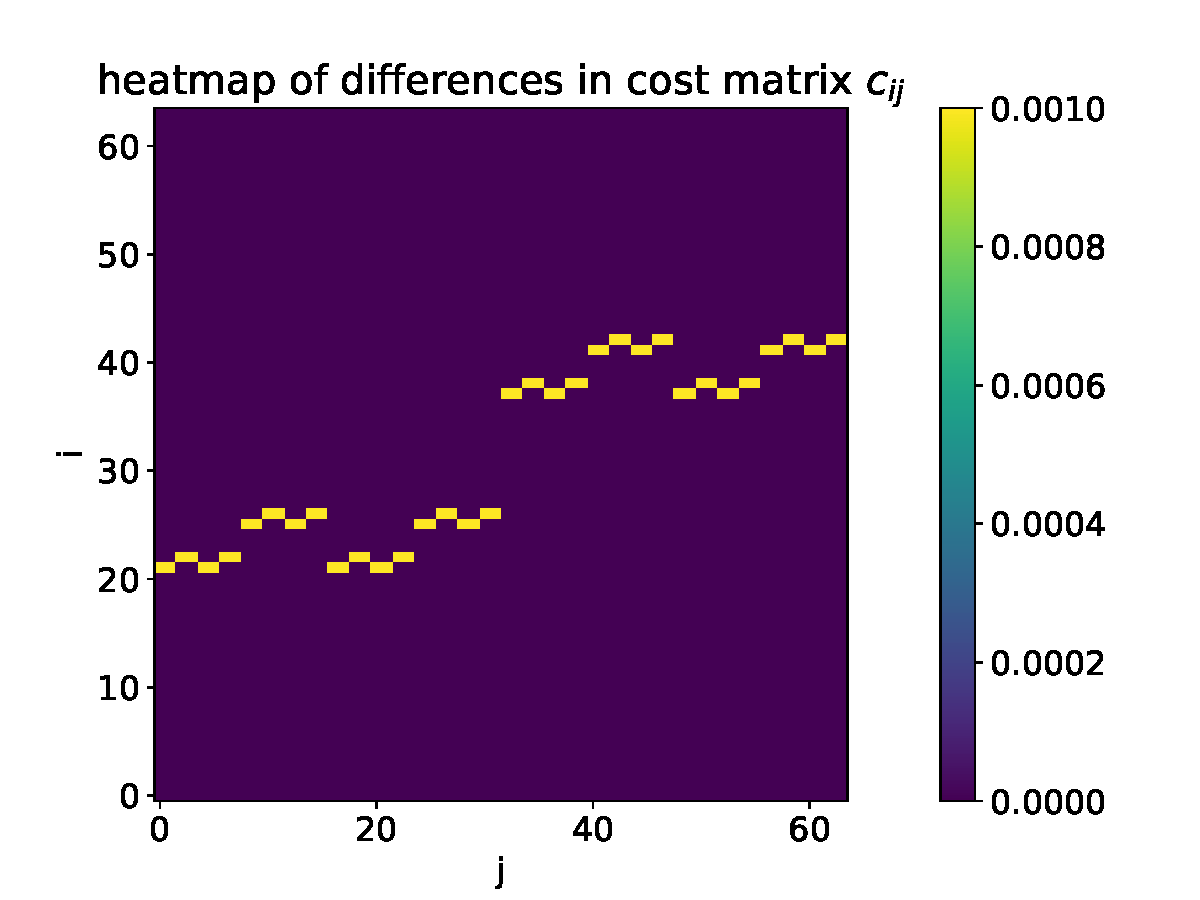
\includegraphics[width=0.5\textwidth]{./images/nonuniform_expansion_ma_n4_c-M10-exp2-newdiff.pdf}\label{fig:madiff1}}
	\subfloat[Non-uniform collapse.]{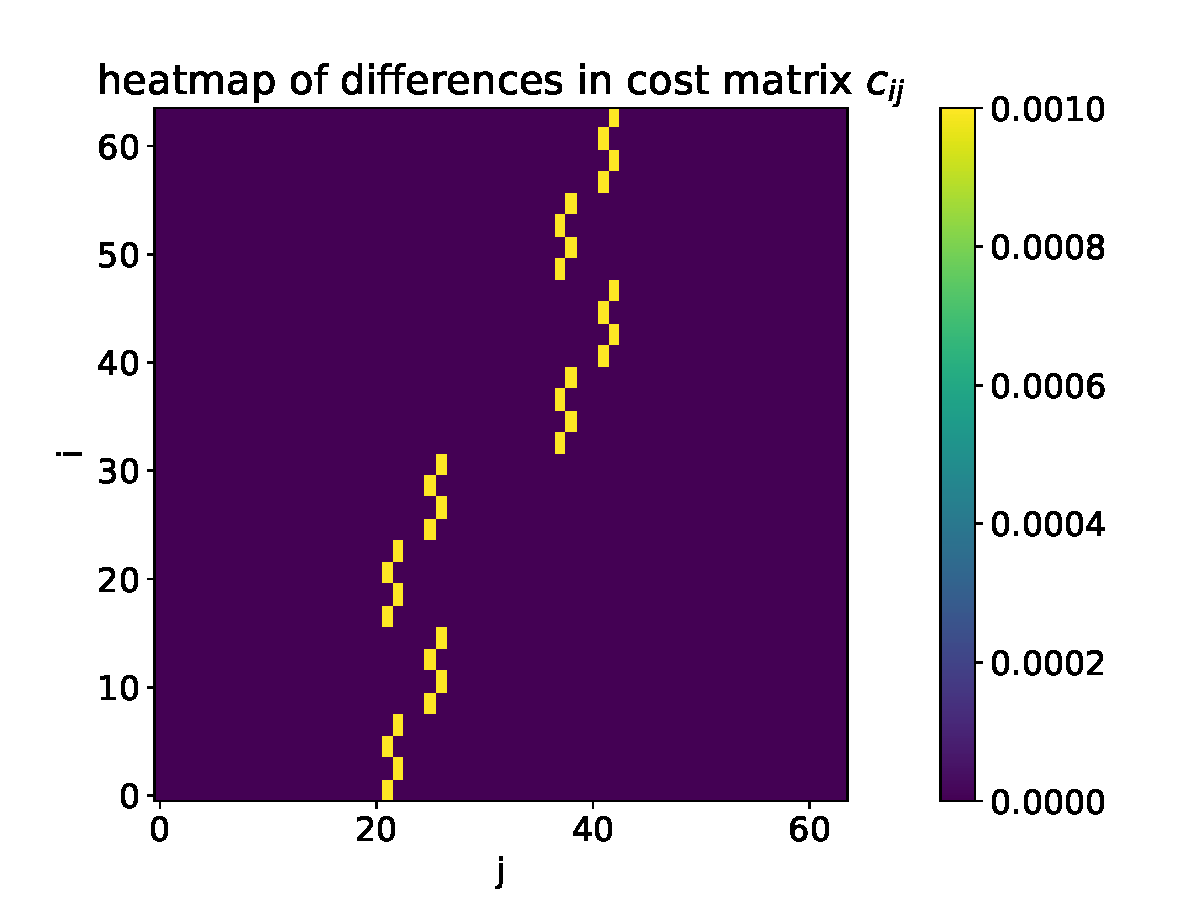
\includegraphics[width=0.5\textwidth]{./images/nonuniform_collapse_ma_n4_c-M10-exp2-newdiff.pdf}\label{fig:madiff2}}
	\caption{Heat map of the differences in the cost matrix for non-uniform expansion (left) and collapse (right) from Algorithm~\ref{alg:1} and the algorithm from \citet{ma2021}, for \lstinline|exp| $=2$ and $n = 4$.}
	\label{fig:madiff}
\end{figure}

\chapter{Additional Reference Cases}
\label{sec:apprefs}
In this appendix, we will discuss some more reference cases. Algorithm~\ref{alg:1} is used to find the cost matrix of the simulations, with $R(c) = \mathbbm{1}_U$, and $U = [0, M_c]^3$, as in Chapter~\ref{ch:results}. We choose $\gamma = \varepsilon = 1$ and $M_c = 10$. To better see differences in the heat map of the acquired cost matrix, we manually set all entries that were equal to $M_c$, equal to the highest entry of $c$ that is not equal to $M_c$. All reference cases are simulated with one million particles. In all simulations, a box size of $100$ (arbitrary units) is used. \par 
We will look at the $n=8$ case for the references for which it has not been discussed, as well as some values of \lstinline|exp| for $n=4$ which have not been discussed. 

\section{Voids}
First, we look at voids, the non-uniform expansion. All data points start in a cube centered at $(50, 50, 50)$ with sides of $50$, and particles can move towards the whole box. We simulate the same non-uniformity as in Section~\ref{sec:voids}. We look at \lstinline|exp| $=2$ and \lstinline|exp| $=5$ for $n=8$, in Figure~\ref{fig:nonuniformexpn8}. We can see some structure, but notably the \lstinline|exp| $=2$ and \lstinline|exp| $=5$ cases look structure-wise very similar; the only difference is a (not necessarily uniform) scaling. 

\begin{figure}[!ht]
	\centering 
	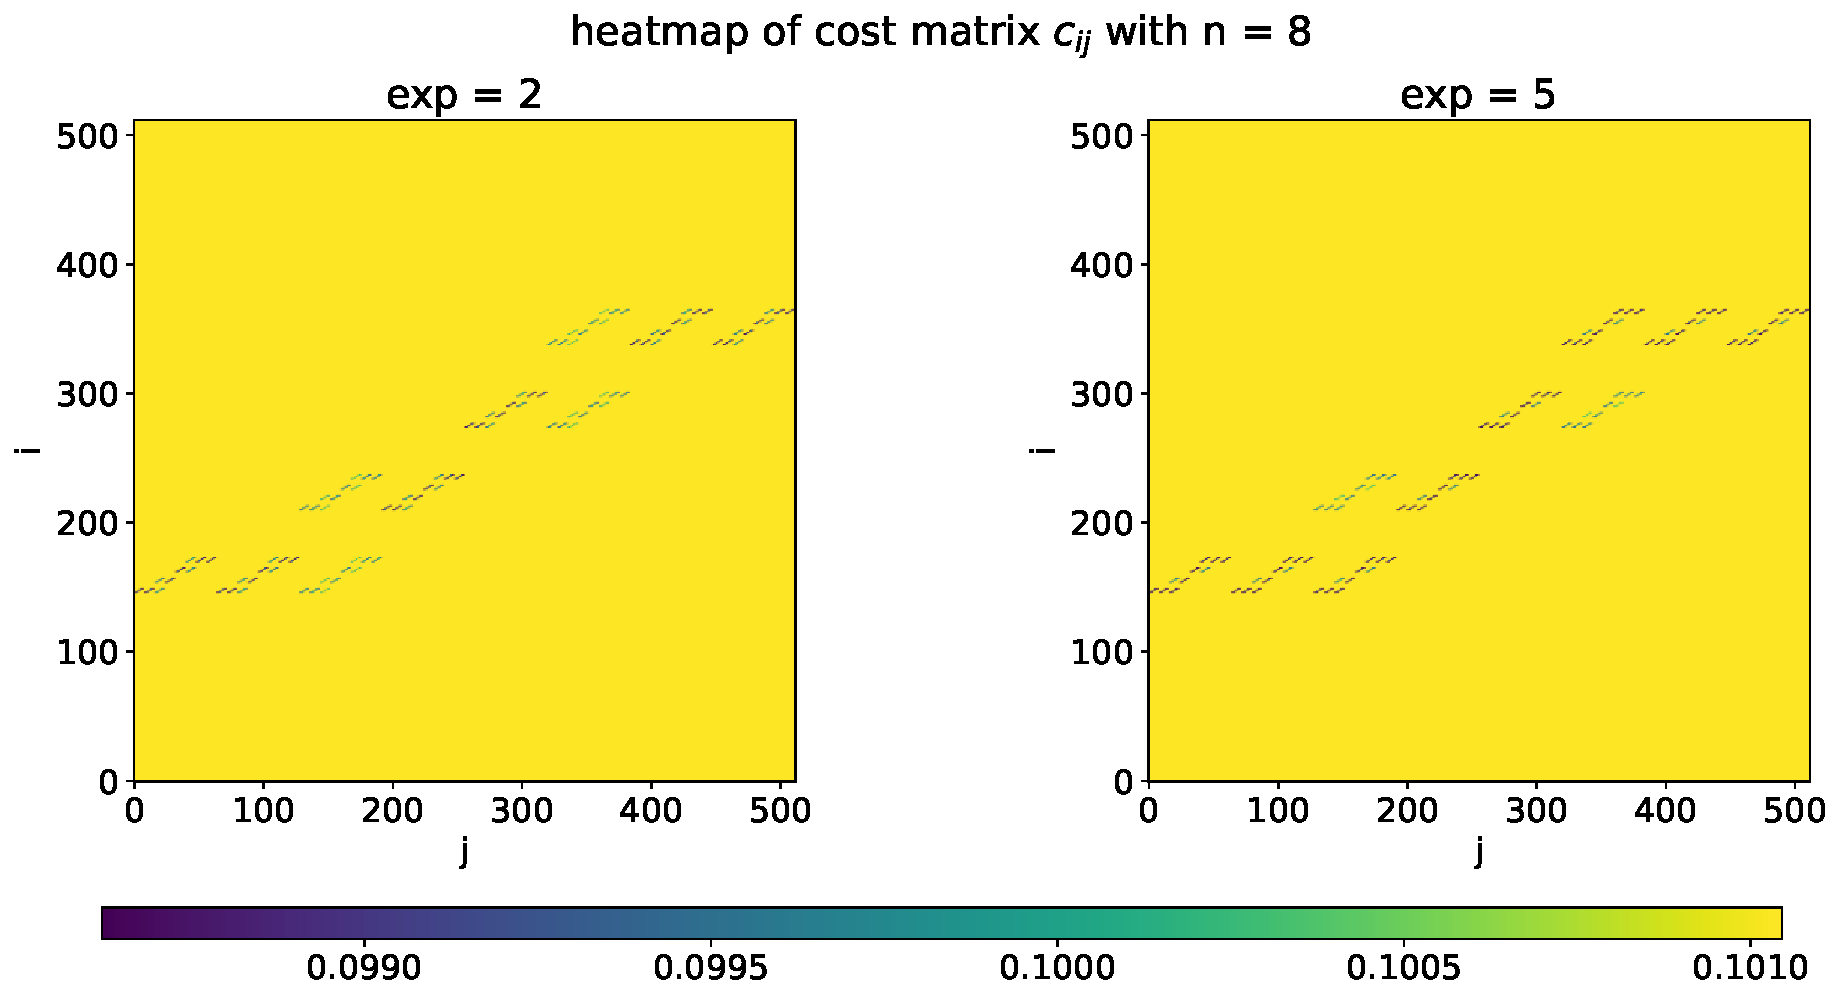
\includegraphics[width=0.8\textwidth]{./images/nonuniform_expansion_ma_n8_c-combined-exp[2, 5]-new.pdf}
	\caption{Heat map of the cost matrix for non-uniform expansion, for both \lstinline|exp| $= 2$ (left) and \lstinline|exp| $=5$ (right), for $n = 8$, as retrieved from Algorithm~\ref{alg:1}. }
	\label{fig:nonuniformexpn8}
\end{figure}

We can also look at other values of \lstinline|exp|. For example, \lstinline|exp| $= 0.4$ for $n=4$ and $n=8$, in Figure~\ref{fig:nonuniformexpn8-new}. We can see that the $n=4$ looks just like another scaling of what we already had in Figure~\ref{fig:nonuniformexpn4}, and the structure in the $n=8$ case is different, but not too different then in the \lstinline|exp| $=2$ or \lstinline|exp| $=5$ case in Figure~\ref{fig:nonuniformexpn4}. 

\begin{figure}[!ht]
	\centering 
	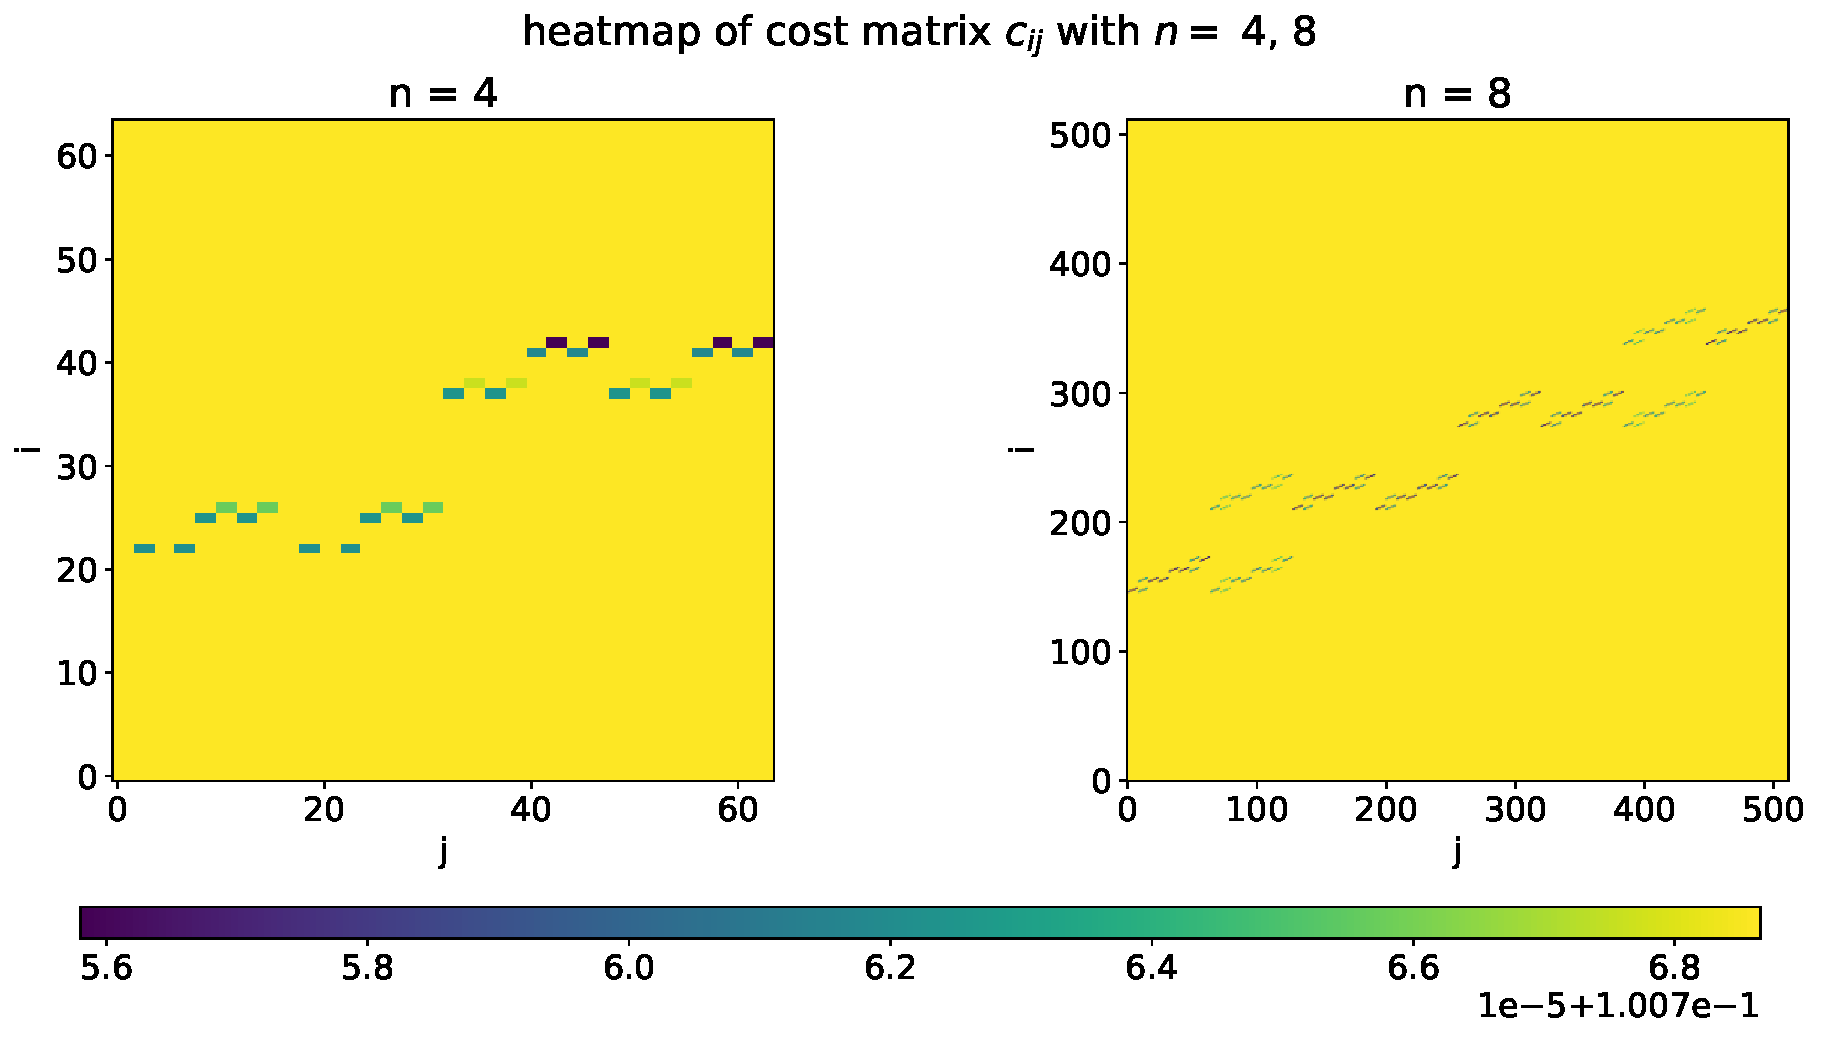
\includegraphics[width=0.8\textwidth]{./images/nonuniform_expansion_ma_ncombined-n8-new.pdf}
	\caption{Heat map of the cost matrix for non-uniform expansion, for \lstinline|exp| $= 0.4$ for both $n=4$ (left) $n=8$ (right), as retrieved from Algorithm~\ref{alg:1}. }
	\label{fig:nonuniformexpn8-new}
\end{figure}

\section{Clusters}
Let us now look at clusters, specifically at the non-uniform collapse. All data points start in the whole cube and will move towards $(50, 50, 50)$, as in Section~\ref{sec:clusters}. We look at \lstinline|exp| $=2$ and \lstinline|exp| $=5$ for $n= 8$, in Figure~\ref{fig:nonuniformcolln8}. \par 
\begin{figure}[!ht]
	\centering 
	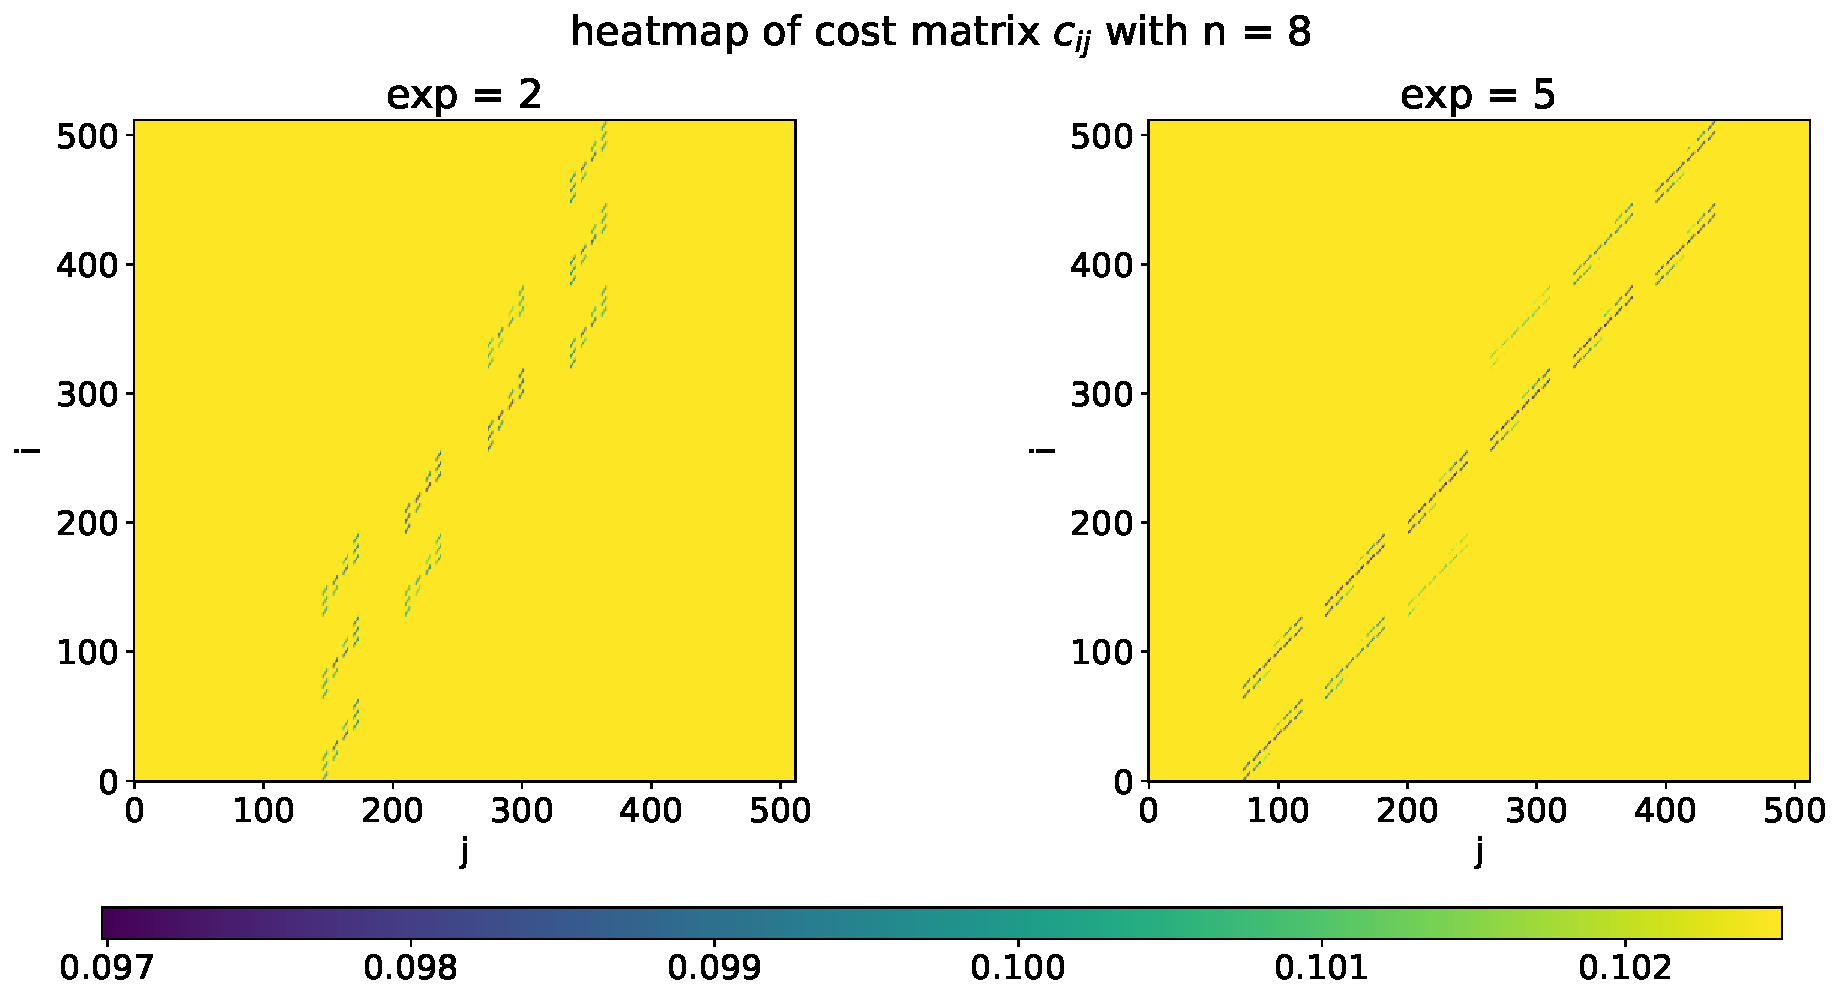
\includegraphics[width=0.8\textwidth]{./images/nonuniform_collapse_ma_n8_c-combined-exp[2, 5]-new.pdf}
	\caption{Heat map of the cost matrix for non-uniform collapse, for both \lstinline|exp| $=2$ (left) and \lstinline|exp| $=5$ (right), for $n = 8$, as retrieved from Algorithm~\ref{alg:1}. }
	\label{fig:nonuniformcolln8}
\end{figure}

In the $n=8$ case for non-uniform collapse, we can see some some structure. Note, however, that the structure is significantly different in the \lstinline|exp| $=2$ case then in the \lstinline|exp| $=5$ case. This could have been expected from the $n=4$ case in Figure~\ref{fig:nonuniformcolln4}, where for a higher value of \lstinline|exp| a more tilted structure can be seen. \par 
We can also look at other values of \lstinline|exp|. For example, \lstinline|exp| $= 0.4$ in Figure~\ref{fig:nonuniformcolln4-new} for $n=4$ and $n=8$. Note that the \lstinline|exp| $= 0.4$ case looks a lot different than any other case, especially for the higher \lstinline|exp|, for both $n=4$ as for $n=8$. This is probably due to the fact that the particle distribution changes as \lstinline|exp| grows. \par 
\begin{figure}[!ht]
	\centering 
	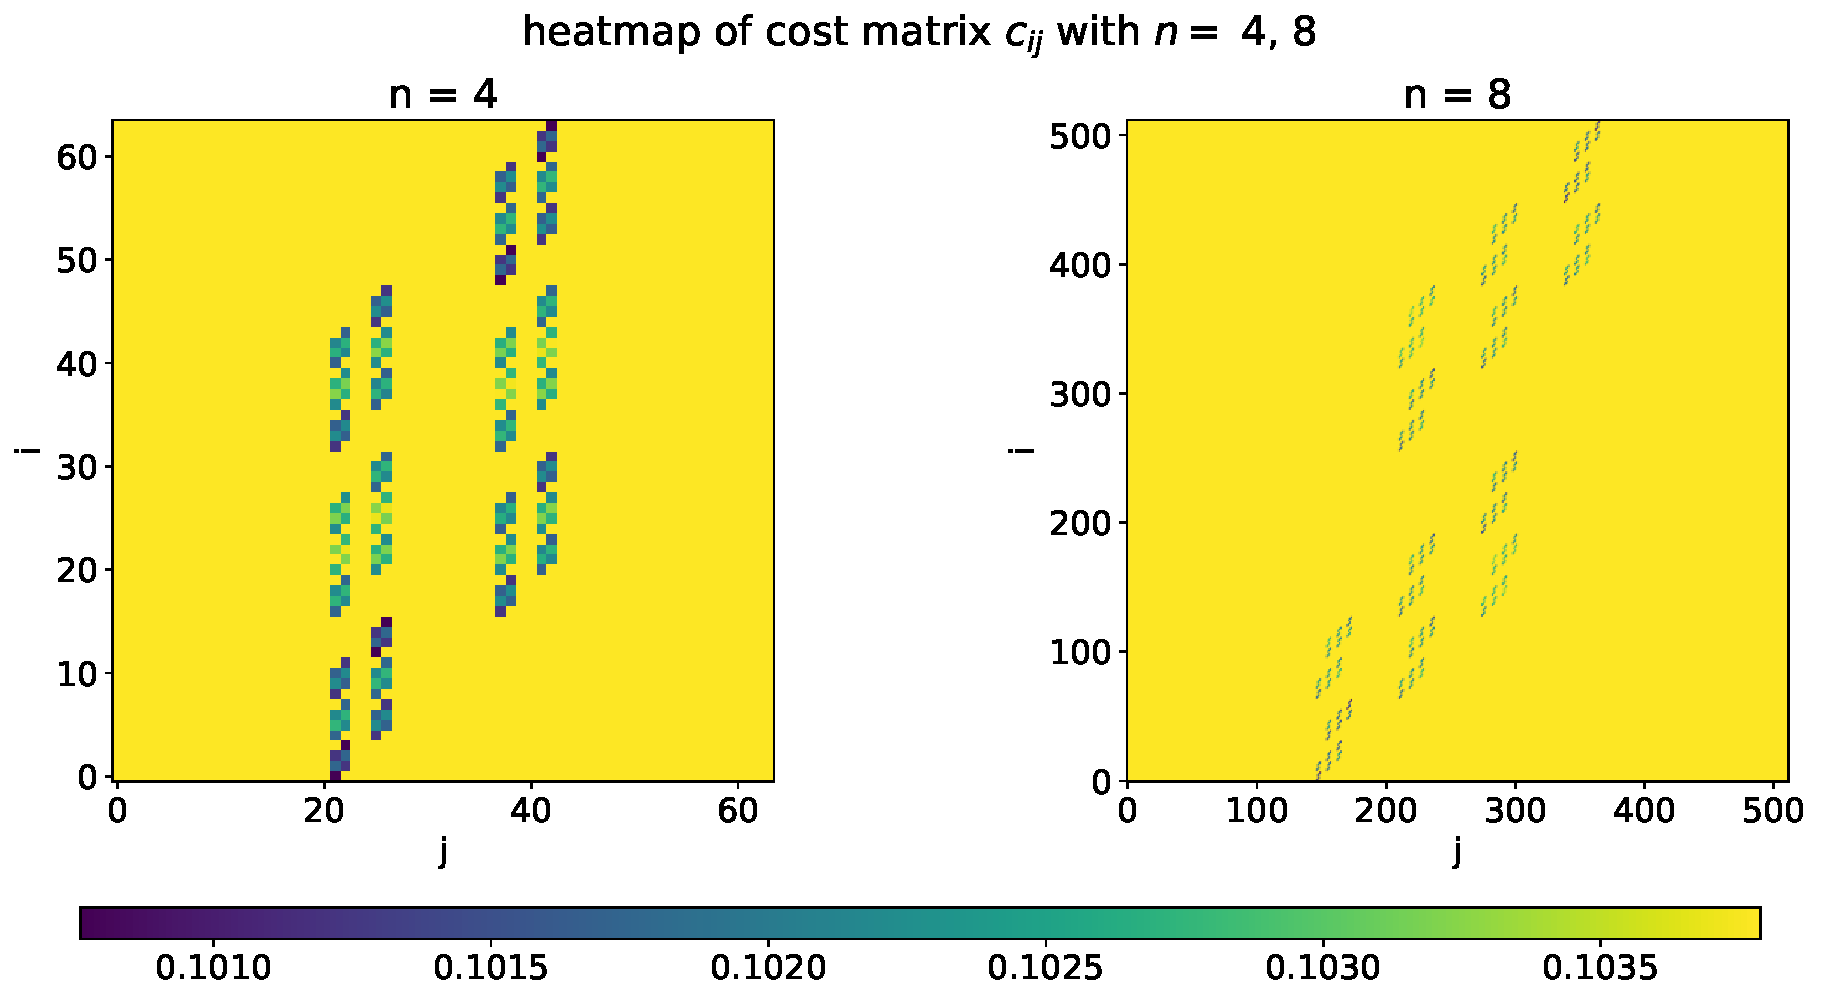
\includegraphics[width=0.8\textwidth]{./images/nonuniform_collapse_ma_ncombined-n8-new.pdf}
	\caption{Heat map of the cost matrix for non-uniform collapse, for \lstinline|exp| $=0.4$, for both $n=4$ (left) and $n=8$ (right), as retrieved from Algorithm~\ref{alg:1}. }
	\label{fig:nonuniformcolln4-new}
\end{figure}

 
\section{Walls and Filaments}
More cases of combinations of expansion and collapse, walls and filaments, were simulated too. All particles start in a cube of length $50$ and can move towards the whole box (of length $100$), as in Section~\ref{sec:refs}. For walls, the cost matrix was calculated for $n=8$, with \lstinline|exp| $=2$ and \lstinline|exp| $=5$, as can be seen in Figure~\ref{fig:walln8}. Notably the \lstinline|exp| $=2$ and the \lstinline|exp| $=5$ do not seem to differ a lot apart from a scaling. \par 
\begin{figure}[!ht]
	\centering 
	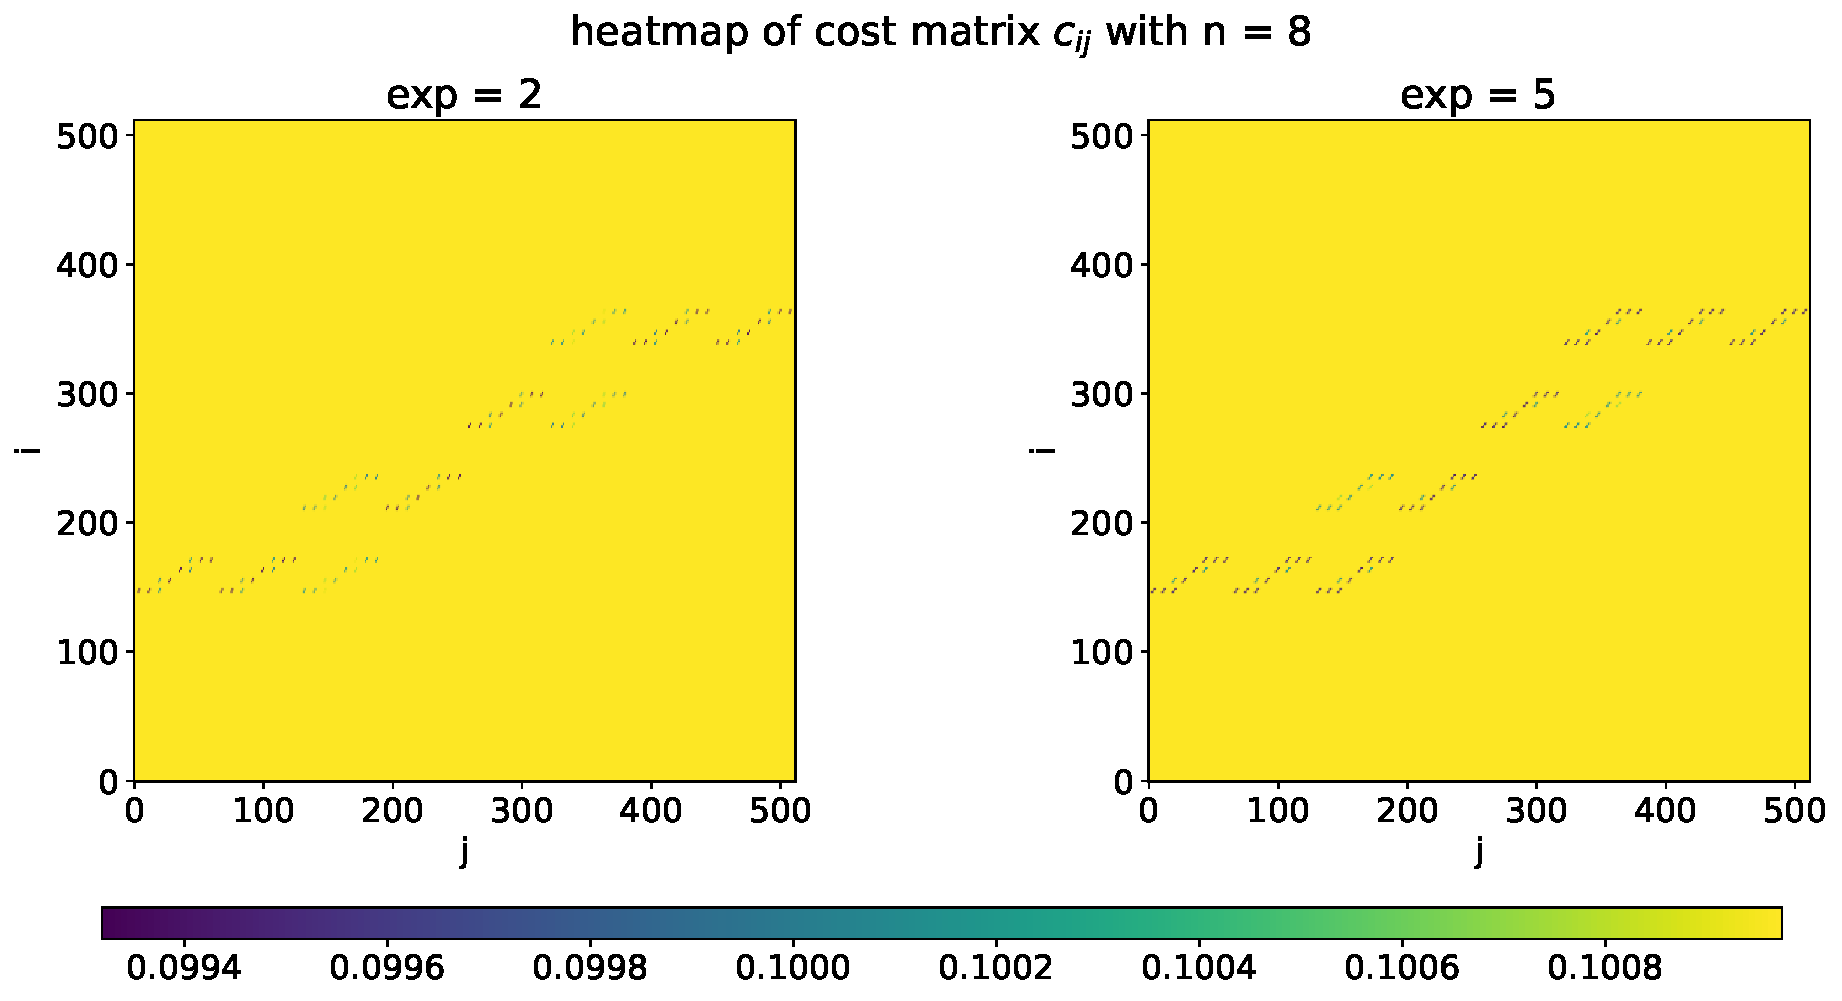
\includegraphics[width=0.8\textwidth]{./images/walls_ma_n8_c-combined-exp[2, 5]-new.pdf}
	\caption{Heat map of the cost matrix for non-uniform collapse, for both \lstinline|exp| $=2$ (left) and \lstinline|exp| $=5$ (right), for $n = 8$, as retrieved from Algorithm~\ref{alg:1}. }
	\label{fig:walln8}
\end{figure}

For filaments, the cost matrix was also calculated for $n=8$, with \lstinline|exp| $=2$ and \lstinline|exp| $=5$, as can be seen in Figure~\ref{fig:filamentn8}. In contrast to the walls, the \lstinline|exp| $=2$ case does look different than the \lstinline|exp| $=5$ case, by a rotation and a lack of some non-$M_c$ entries.
\begin{figure}[!ht]
	\centering
	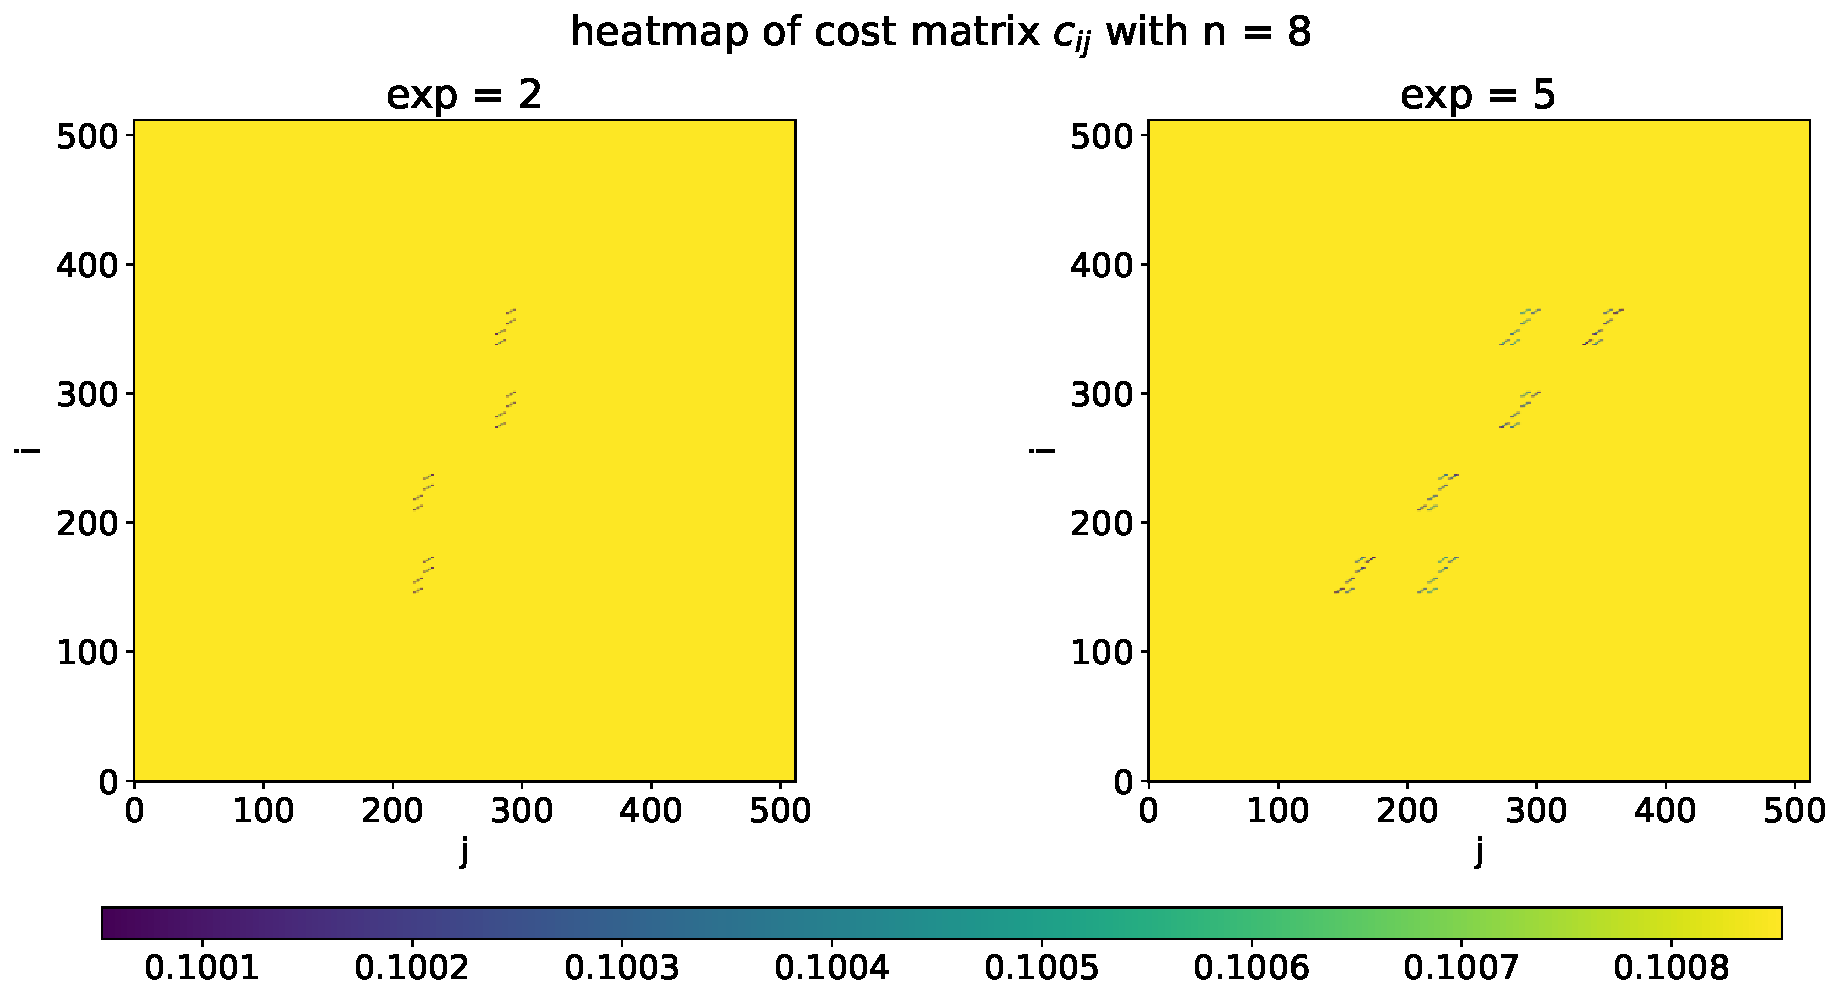
\includegraphics[width=0.8\textwidth]{./images/filament_ma_n8_c-combined-exp[2, 5]-new.pdf}
	\caption{Heat map of the cost matrix for non-uniform collapse, for both \lstinline|exp| $=2$ (left) and \lstinline|exp| $=5$ (right), for $n = 8$, as retrieved from Algorithm~\ref{alg:1}. }
	\label{fig:filamentn8}
\end{figure}




%\chapter[Markov Chain Monte Carlo Simulation Results]{Markov Chain Monte Carlo\\ Simulation Results}

%\chapter{Differences Between $\pihat$ and $c$}









\end{document}

